\RequirePackage[ngerman=ngerman-x-latest]{hyphsubst}
\documentclass[a4paper,12pt,twoside]{article}

\usepackage[ngerman]{babel}
\usepackage{fancyhdr}
\usepackage{graphicx}
\usepackage{subfig}
\setlength\abovecaptionskip{4pt}
\usepackage[bookmarksopen=true,bookmarksnumbered=true]{hyperref}
\newcommand{\subfigureautorefname}{\figureautorefname}
\usepackage[utf8]{inputenc}
\usepackage[inner=2.5cm,outer=2cm,top=2.3cm,bottom=2cm,head=0.8cm,headsep=0.8cm,footskip=1cm,asymmetric]{geometry}
\usepackage{setspace}
\usepackage{courier}
\usepackage{array}
\usepackage{amsmath}
\usepackage{amssymb}

\usepackage[babel, german=quotes]{csquotes}

\usepackage[backend=biber,style=apa, language=autocite, doi=false, isbn=false]{biblatex}
\addbibresource{master.bib}
%\bibliography{master.bib}
\DeclareLanguageMapping{ngerman}{ngerman-apa}

\newcommand{\Fb}[1]{\textit{#1}} %Fachbegriff



\usepackage{listings}
\usepackage[dvipsnames]{xcolor}
\lstset{ % 
  %language=C++,                % the language of the code 
  frame=single,
  basicstyle=\footnotesize,           % the size of the fonts that are used for the code 
  numbers=left,                   % where to put the line-numbers 
  numberstyle=\tiny\color{gray},  % the style that is used for the line-numbers 
  stepnumber=2,                   % the step between two line-numbers. If it's 1, each line 
                                  % will be numbered 
  numbersep=5pt,                  % how far the line-numbers are from the code 
  backgroundcolor=\color{white},      % choose the background color. You must add \usepackage{color} 
  showspaces=false,               % show spaces adding particular underscores 
  showstringspaces=false,         % underline spaces within strings 
  showtabs=false,                 % show tabs within strings adding particular underscores 
  rulecolor=\color{black},        % if not set, the frame-color may be changed on line-breaks within not-black text 
  tabsize=2,                      % sets default tabsize to 2 spaces 
  captionpos=b,                   % sets the caption-position to bottom 
  breaklines=true,                % sets automatic line breaking 
  breakatwhitespace=false,        % sets if automatic breaks should only happen at whitespace 
  title=\lstname,                   % show the filename of files included with \lstinputlisting; 
                                  % also try caption instead of title 
  keywordstyle=\color{blue},          % keyword style 
  commentstyle=\color{PineGreen},       % comment style 
  stringstyle=\color{Orchid},         % string literal style 
  escapeinside={\%*}{*)},            % if you want to add a comment within your code
  aboveskip=20pt
} 
%\usepackage[german]{babel}
\addto\extrasngerman{%
	\def\subsectionautorefname{Abschnitt}%
	\def\subsubsectionautorefname{Abschnitt}%
}

% Nummer des Themas
\newcommand{\No}{$136$}
% Name des Themas
\newcommand{\Theme}{Multi-threaded Query Processing II}
% Name   
\newcommand{\Name}{Ingo Bader}

\onehalfspacing

\nopagebreak

\fancyhead[RE,LO]{\fontsize{9}{9}\selectfont\Theme}
\fancyhead[LE,RO]{\fontsize{9}{9}\selectfont Seite \thepage}
\fancyfoot{}

\begin{document}


% Titelseite
\thispagestyle{empty}
\pagestyle{empty}

\begin{center}
\begin{huge}
\vspace*{3cm}
%      \vspace*{\fill}
    \begin{tabular}{m{1.2cm}@{\ \ }m{9cm}}
      
\includegraphics[width=1.2cm]{logo.eps} & {FernUniversität in Hagen}
    \end{tabular}
    \\
    \vspace*{3cm}
   Masterarbeit \\
   Sommersemester 2020 \\[2em]
   \glqq{} \Theme \grqq{} \\[2cm]
\end{huge}
\begin{large}
	\Name \\[3cm]
   	Betreuer \\[1em]
   	Prof. Dr. Ralf Güting 
\end{large}
\end{center}

\clearpage
\tableofcontents
\clearpage
\raggedbottom
\thispagestyle{fancy}
\pagestyle{fancy}
\setcounter{page}{1}

% Inhalt
\section{Einleitung} (2-3 S)n

Die in Datenbanksystemen gespeicherten Daten werden immer umfangreicher und auch komplexer. Einerseits ist Big Data in den letzten Jahren ein wichtiges Thema geworden und andererseits werden Datentypen wie räumliche Daten, Bilder oder Dokumente in Datenbanken gespeichert und verarbeitet, die wesentlich mehr Speicher benötigen als klassische Datenbankobjekte. Dementsprechend gewinnt die Verarbeitungsgeschwindigkeit, in der Datenbankoperationen ausgeführt werden können, immer mehr an Bedeutung. Gleichzeitig haben Mehrprozessor- oder Mehrkernsysteme seit mehr als einem Jahrzehnt auch jenseits sehr spezialisierter Systeme an Verbreitung gewonnen, während der Taktfrequenz eines einzelnen Prozessorkerns inzwischen an die physikalischen Grenzen gestoßen ist.

Dementsprechend liegen Ansätze nahe, insbesondere für Nicht-Standard-Datenbankanwendungen, also welchen, deren Daten von den Standardtypen relationaler Datenbanksysteme abweichen, die Anfragen parallel zu bearbeiten, um die Rechenlast auf verschiedene Kerne, Prozessoren oder Systeme zu verteilen. In Secondo implementiert ist eine Algebra, die es ermöglicht, Anfragen auf verteilten, lose gekoppelten Systemen mit jeweils eigenem Hauptspeicher und Speichermedien auszuführen.

Innerhalb nur eines Computersystems sind zwei Herangehensweisen denkbar: Die einzelnen Operatoren eines Operatorenbaums können parallelisiert werden. Mit diesem Ansatz ist es möglich, sowohl Operatoren in einer Pipeline-Parallität abzuarbeiten als auch Daten mit expliziten Partitionierungs-Operatoren aufzuteilen und dann die entsprechenden Pakete parallel abzuarbeiten. Der Ansatz ist vergleichbar mit den verteilten Systemen, nur ist meist der Speicher geteilt, aber die Kommunikationskosten zwischen den einzelnen Prozessen fallen nicht so stark ins Gewicht. Vorteil dieser Herangehensweise ist es, dass sich für den Nutzer nicht unbedingt etwas ändern muss, sondern der Optimierer die Entscheidung übernehmen kann, wie parallelisiert wird. Auch kann der ganze Umfang von Algebren und Operatoren genutzt werden. In Secondo ist dieser Ansatz in der ParThread-Algebra umgesetzt.

Hier soll eine anderer Herangehensweise verfolgt werden, Parallelität zu implementieren. In der MThreaded-Agebra werden explizit parallele Operatoren entworfen und implementiert. Dieser Ansatz verspricht einen größeren Performancegewinn, da auf Parallelität optimierte Algorithmen entwickelt werden können. Konnten in dem anderen Verfahren nur eine äußere Partitionierung bzw. ein Pipelining eingesetzt werden, besteht mit diesem Ansatz die Möglichkeit, Lastenverteilung intern zu optimieren und enger gekoppelte parallele Operationen zu entwerfen. Verloren geht dagegen die Flexibilität des Ansatzes einer äußeren Integration paralleler Verarbeitung, da nur explizit parallel entworfene Operatoren für eine parallele Verarbeitung genutzt werden können. Auch ein paralleler Pipeline-Prozess ist mit diesem Ansatz nicht mehr möglich.

Das Ziel dieser Arbeit ist es also, neue parallele Operatoren zu entwerfen. Um für diesen Ansatz geeignet zu sein, müssen Opertoren zwei Bedingungen erfüllen: Es muss Algorithmen für die gewählten Operatoren geben, die sich für eine Parallelisierung eignen und die ausgeführten Berechnungen müssen eine Komplexität aufweisen, für die sich für die Verwaltung der Threads und die Datenaufteilung der Mehraufwand lohnt. Ich habe mich dafür entschieden, einen Sort-Operator, einen Equi-Join und einen Spatial Join zu entwickeln. Für diese Operatoren treffen die genannten Bedingungen zu und sie werden zugleich häufig in Datenabfragen angewandt. Umgesetzt wird die Implementierung in dem Secondo-Datenbanksystem mit C++11, indem eine neue Algebra entworfen wird: die MThreadedAlgebra. 

Beginnen werde ich mit einer Reflexion des Forschungsstandes und werde dabei allgemein die Debatte um Parallelisierung bewerten, speziell auf deren Anwendung in Datenbanksystemen eingehen und Ansätze für eine Parallelisierung von Sort-, Join- und Spatial-Join-Operatoren bewerten. Ausgehend von der Darstellung des momentanen Forschungsstandes werde ich bei der Entwicklung der genannten Operatoren in zwei Schritten vorgehen: Einem Entwurf der Operatoren zusammen mit einer Diskussion des verfolgten Ansatzes und dem folgend einer Reflexion der Implementierung der entsprechenden Operatoren. Eine Bewertung des Ergebnisses findet experimentell in mehreren Schritten statt: Eine gute Funktionsweise der Operatoren bedeutet Korrektheit, Robust und Effizienz. Zur Betrachtung der Effizienz findet ein Vergleich statt mit den Single Thread-Versionen der Operatoren, aber auch anderen parallelen Implementierungen. Dem folgend wird das Verhalten der Operatoren bei einer Veränderung von Parametern wie Kernzahl, Arbeitsspeicher oder Verteilung innerhalb von Relationen betrachtet.

\section{Grundlagen}
1/4 (15 S.)

\subsection{Secondo} (1 S)

In meiner Arbeit werde ich Konzepte und eine Implementierung paralleler Datenbankoperatoren vorstellen und ausgewählte Operatoren in dem Secondo-Datenbanksystem entwickeln. Secondo {\autocite{Gueting2010}} ist ein erweiterbares Datenbanksystem, das von der Fernuniversität Hagen entwickelt worden ist, um Datentypen, die keine Standard-Datentypen wie räumliche und raum-zeitliche Typen sind, zu implementieren und mit ihnen zu experimentieren, die keine Standard-Datentypen sind, vor allem räumliche und raum-zeitliche Typen. Die Architektur von Secondo besteht aus drei zentralen Komponenten: dem Kernel, dem Optimizer und der GUI. Der Secondo-Kernel ist die Schicht zwischen der Berkley-DB, auf die Secondo aufsetzt und GUI sowie Optimizer {\autocite{Gueting2017}}. Sie beinhaltet Algebren bestehend aus Typen und Operatoren. Die Schichten, die zwischen GUI und den Algebren vermitteln, sind der Query-Prozessor, -Katalog und der Command-Manager. Der Storage-Manager und weitere Tools dienen als Schnittstelle zu der zugrundeliegenden Datenbank. Durch die offen gestaltete und klar definierte Schnittstelle zur Integration neuer Algebren bestehend aus Typkonstruktoren und dazugehörigen Operatoren hat Secondo eine sehr große Flexibilität bezüglich unterschiedlicher Datentypen und Funktionalitäten. Darüber hinaus ist es nicht auf einen Datenmodell festgelegt, auch wenn die meisten Implementierungen vor allem ein relationales bzw. objekt-relationales Datenmodell unterstützen. Der Optimizer unterstützt ausschließlich ein relationales Datenmodell. 

\begin{figure}
	\centering
	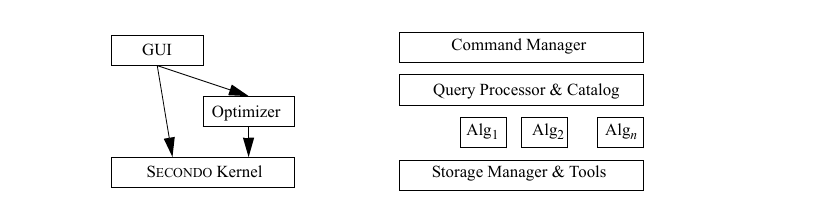
\includegraphics[width=0.75\textwidth]{Bilder/secondo.png}
	\caption{SECONDO Komponenten und Architektur des Kernels \autocite{Gueting2010}}
	\label{img:secondo}
\end{figure}

Abstract Data Types (ADT) fassen Datentypen mit dazugehörigen Operationen zusammen und ermöglichen es, beispielsweise räumliche Datentypen gemeinsam mit den notwendigen Operationen zu entwerfen, ohne sich bereits über die Implementierung und detailierte Struktur der Datentypen Gedanken zu machen. {\textcite[S. 75ff]{Rigaux2001}} beschreibt, wie ADTs für räumliche Datentypen entworfen werden können. Secondo setzt dieses Konzept weitestgehend um. Die \Fb{SpatialAlgebra} bietet darüber hinaus ein ausreichendes Set topologischer Prädikate, um hinreichend räumliche Beziehungen zwischen Punkten, Sets von Punkten, Linien und Regionen/Polygonen zu beschrieben.

Wichtig für die von mir zu entwickelnde Algebra sind mehrere Bestandteile von Secondo. Die Relational-Algebra stellt das relationale Datenmodell inklusive des Datentyps Tupel und Persistierungsstrukturen für Tupel zur Verfügung. Die Stromverarbeitung ermöglicht es, große Sätze von Daten in einer Pipeline zu verarbeiten; in meinem Fall in Tupelströmen. Fake Large Objects (FLOBs) ermöglichen es, Instanzen von Typen mit variabler Größe zu implementieren, indem es abhängig von der Größe ein Objekt entweder Teil des Tupel ist oder separat gespeichert wird. Unter Anderem für räumliche Datentypen sind solche Möglichkeiten essentiell. Für einen schnellen Zugriff werden zum Beispiel räumliche Datentypen variabler Größe durch ihre minimale Bounding Box direkt im Tupel repräsentiert. Ein FLOB hat also immer eine Repräsentation in dem Teil des Tupel zu sein, der in den Hauptspeicher geladen wird, der aber im Gegensatz zu den beliebig großen Objekten klar begrenzt ist \autocite{Gueting2010}.

Der \Fb{Command-Manager} bietet neben einer dem SQL-Standard entsprechenden Abfragesprache eine zweite, "executable" Abfragesprache genannte Sprachebene, die in ihrer Abstraktion zwischen SQL und einer Programmiersprache wie C++ steht. Mit dieser Abfragesprache können Anfragen direkt an den Kernel gestellt werden und dementsprechend steht nur auf dieser Ebene der volle Funktionsumfang des Kernels zur Verfügung. Allerdings ist SQL deutlich einfach benutzbar \autocite{Gueting2010}. 

Bereits jetzt sind Ansätze paralleler Datenverarbeitung in Secondo integriert. Die \Fb{DistributedAlgebra} {\autocite{Nidzwetzki2017}} ermöglicht eine Verarbeitung eines verteilten Anfrageprozesses, indem mehre Secondo-Instanzen auf einem oder mehreren Computern genutzt werden. Verteilte Datenverarbeitung ist so möglich, indem Anfragen partitioniert werden und nach Verarbeitung die Teilergebnisse wieder zusammengeführt werden. Einen Schritt weiter geht die erst kürzlich implementierte ParThread-Algebra, die eine Parallelisierung innerhalb einer Instanz für den Benutzer verborgen vornimmt, indem der Operatorenbaum möglichst optimal für eine parallele Verarbeitung umgeformt wird.

\subsection{Multiprozessorsysteme} (2 S)

Für eine späteres Verständnis des Performance-Verhaltens der von mir entworfenen Operatoren ist ein grundlegendes Verständnis der Funktionsweise und des Aufbaus von Mehrkernprozessoren notwendig. Multiprozessorsysteme grenze ich hier ab von verteilten Systemen. Während in ersteren die verschiedenen Kerne bzw. Prozessoren in einem Computer integriert sind und sich Speicher wie auch die anderen Komponenten teilen, bestehen verteilte Systeme aus unabhängigen Computer, die über ein Netzwerk miteinander verbunden sind. Man spricht auch von enger und loser Kopplung. Dementsprechend sind in verteilten Systemen die Kommunikationskosten zentral für die Bestimmung der Performance. Als weitgehend identisch betrachte ich für meine Fragestellung Mehrkern- und Mehrprozessorsysteme. Einziger Unterschied ist meist die Aufteilung des Caches auf mehrere Prozessoren bei Mehrprozessorsystemen, aber auch einzelne Komponenten können unabhängig voneinander sein. In älterer Literatur wird meist von Mehrprozessorsystemen gesprochen, da Mehrkernprozessoren eine relativ neue Entwicklung sind. Eingehen werde ich hier nur auf Mehrkernprozessoren.

In der Flynn’sche Taxonomie paralleler Architekturen, die globale Kontrolle und resultierender Daten sowie Kontrollflüssen zwischen den Prozessen betrachtet, entsprechen Mehrkern- und auch Mehrcomputersysteme einer Multiple Instruction, Multiple Data (MIMD) Rechnerarchitektur {\autocite[S. 10f]{Rauber2013}}. Andere Architekturen sind beispielsweise für die parallele Bearbeitung von Bilddaten auch in Desktop-Computern relevant.

Ab 2005 war eine Leistungssteigerung von Einkernprozessoren wegen der entstehenden Abwärme nicht mehr in großem Umfang technisch möglich. Anstatt vor allem auf die Steigerung des Prozessortakts zu setzen, wurden ab dieser Zeit Prozessoren mit mehreren unabhängigen Einheiten, Kerne genannt, entwickelt, die ab 2009 Standard in Desktopcomputersystemen wurden. Die CPU-Kerne haben eigene Registersätze und arithmetisch-logischer Einheiten (ALU), nur der Bus und einige Caches werden von mehreren Kernen geteilt. Die Leistungssteigerung von Computerprogrammen wurde dementsprechend abhängig von einer parallelen Ausführung von Programmeinheiten. Standard-Desktopprozessoren unterliegen einem hierarchisches Design. Für die Performance von Multiprozessor-Algorithmen ist eine optimale Nutzung der Kern-spezifischen L1/L2-Caches und dem geteilten L3-Cache wichtig {\autocite{Rauber2013}}. Der Cache enthält exakte Kopien von Daten und Befehlssätzen aus dem Hauptspeicher, die besonders häufig genutzt werden. Der L1-Cache ist am schnellsten, aber meistens nicht sehr groß. Befehls- und Datencache ist hier getrennt. In einigen Systemen hat nicht jeder Kern die vollständige Funktionalität eines Prozessors, sondern bestimmte Ressourcen, wie eine Gleitkommaeinheit, werden geteilt von mehreren Kernen. Beispielsweise sind in der AMD-FX-Architektur zwei Kerne mit je eigener Integereinheit und eigenem L1-Cache zu einem Modul mit geteilter Gleitkommaeinheit und geteiltem L2-Cache zusammengefasst. Hyperthreading ist eine Technik, mehrere Threads auf einem Kern gleichzeitig auszuführen und so zu koordinieren, dass die Ausführung schneller ist, als wenn die Threads seriell ausgeführt würden. Diesen Ausführungen folgt, dass die Performance auch vollständig unabhängige Threads ohne Overhead nicht unbedingt linear wächst bei einer steigenden Anzahl von Kernen, da Kerne sich teils Ressourcen teilen.

Parallele Ausführungen kann es mit unterschiedlicher Kopplung geben. Man unterschiedet zwischen Threads und Prozessen. Threads sind über einen eigenen Kontrollfluss definiert. Sie haben einen unabhängiger Registersatz inkl. Instruction Pointer, einen eigenen Stack, aber im Gegensatz dazu verfügen Prozesse über einen eigenen Adressraum {\autocite[S. 95]{Rauber2013}}. Die meisten Betriebsmittel werden von allen Threads gemeinsam verwendet. Durch die gemeinsame Nutzung von Betriebsmitteln kann es auch zu Konflikten kommen. Diese müssen durch den Einsatz von Synchronisationsmechanismen aufgelöst werden.

\subsection{Parallele Algorithmen} (2 S)

Warum aber wird eine Parallelisierung nicht automatisch vorgenommen? Die ParThreaded-Algebra, die bereits in Secondo implementiert ist, verfolgt beispielsweise
diesen Ansatz: Sie stellt Operatoren zur Verfügung, um bereits implementierte Single Thread-Operatoren parallel ausführen zu können. Am Beispiel eines parallelen (internen) Merge-Sort zeigt {\textcite{McCool2012}}, warum es oft besser ist, einen neuen parallelen Algorithmus zu suchen anstatt einen seriellen zu parallelisieren. Meistens lohnt es sich also, explizit parallel Operatoren zu entwerfen.

{\textcite[S.104]{Rauber2013}} unterscheidet parallele Programmiermodelle nach folgenden Kriterien:

\begin{itemize}
	\item Befehlsebene, Ebene des Befehlsblocks, prozedurale Ebene oder parallelen%parallele 
	Schleife
	\item implizite oder explizite Parallelität
	\item synchron oder asynchron
	\item Kommunikationsmuster: explizite Kommunikation oder geteilte Variablen
	\item Synchronisationsmechanismen
\end{itemize} 

Greifen sogenannte kritische Bereiche auf gleiche Daten zu, müssen die Zugriffe synchronisiert werden, da es zu Deadlocks oder zu kritischen Wettlaufsituation (race conditions) kommen kann. Von einem Deadlock spricht man, wenn zwei Prozesse auf jeweils eine Sperre warten, aber die genau andere Sperre besitzen. So kommt es zu einer Verklemmung. Sofern in parallelen Algorithmen auf gemeinsame Daten zugegriffen wird, kann die Ausführungsreihenfolge das Ergebnis bestimmen, was als Wettlaufsituation bezeichnet wird. Locks stellen Sperren zur Verfügung, sorgen also dafür, dass eine Aktion atomar ist, und Mutexe sichern den ausschließlichen Zugriff auf kritische Daten, garantieren also, dass ein Zugriff atomar stattfindet {\autocite{Rauber2013}}. Eine Kommunikation zwischen den Threads findet entweder über Nachrichten oder globale Variablen statt. Mit diesen Mitteln kann eine Prozesssynchronisation vorgenommen und sichergestellt werden, dass die einzelnen Aktionen der Threads konsistenzerhaltend sind.

Die Entwicklung einer parallelen Problemlösung wird beeinflusst von der Struktur des Problems und der Daten. Wenn sich ein Problem in Teilprobleme ohne funktionale Abhängigkeit zerlegen lässt, spricht man von inhärenten Parallelismus {\autocite[S. 321f]{Bengel2008}}. Da in diesem Fall wenig Kommunikation zwischen den Prozessen notwendig ist, wird theoretisch ein nahezu lineare Performancegewinn ermöglicht. Eine Zerlegung in Teilprobleme kann über eine Aufteilung der Daten stattfinden, also über eine Partitionierung. Bei einer funktionalen Zerlegung eines Problems in mehre Arbeitsschritte, die nacheinander ausgeführt werden, spricht man von Pipelining {\autocite[S. 324]{Bengel2008}}. Verteilte beziehungsweise parallele Algorithmen haben im Gegensatz zu zentralen keinen globalen Zustand und keine gemeinsame Zeit. Dementsprechend kann es zu unvorhersehbaren Abläufen kommen. Eine Rechenlastverteilung kann statisch oder dynamisch vorgenommen werden {\autocite{Bengel2008}}.

Im Folgendem beschreibe ich einige Architekturmuster, die häufig im Entwurf paralleler Problemlösungen Anwendung finden. Im Fork-Join-Muster werden Threads für bestimmte Aufgaben erzeugt und hinterher wieder zusammengefügt {\autocite[S. 109]{Rauber2013}}. Im Master-Worker-Schema verteilt ein Master Teilbereiche von Daten an mehrere Worker und sammelt die Ergebnisse wieder ein. Der Master übernimmt also ein Scheduling im Gegensatz zum Fork-Join-Muster, welches ohne eine zentrale Instanz auskommt. Der Weg von einer Zerlegung eines Problems zu einer Allokation der Teilprobleme auf Prozessoren kann in vier Schritten beschrieben werden: Partitionierung, Auslegung der Kommunikation, Agglomeration und Mapping. Unterschieden werden hier Ansätze mit viel oder wenig Kommunikation und Parallelisierung {\autocite[S. 326f]{Bengel2008}}. Im bereits erwähnten Pipelining-Archtitekturmuster findet eine funktionale Zergliederung des Problems statt und die Daten werden nacheinander in einer Kette von Threads verarbeitet {\autocite[S. 111]{Rauber2013}}. Im Producer-Consumer-Muster gibt es mehrere Threads, die Daten erzeugen, und mehrere, die Daten erhalten. Eine Kommunikation findet über Buffer statt  {\autocite[S. 112]{Rauber2013}}.

In der Performance-Analyse wird unterschieden zwischen Kosten, Beschleunigung und Effizienz unter Verwendung des PRAM-Modells (paralleler RAM). Das Performance-Verhalten bei wachsender Anzahl von Prozessoren wird Skalierbarkeit genannt {\cite{Rauber2013}}. Beschleunigung beschreibt den Faktor, um den eine Ausführung auf mehreren Workern schneller wäre als auf einem, Effizienz die Beschleunigung pro Worker {\autocite[S. 56]{McCool2012}}. Fallstricke paralleler Programmierung liegen in einer gedrosselten Skalierung, also einem nicht-linearen Anstieg der Performance mit der Anzahl genutzter Kerne verursacht unter anderem durch eine unausgeglichene Lastenverteilung oder durch einen großen Overhead für die Verwaltung der parallelen Prozesse {\autocite[S. 74]{McCool2012}}.

\subsection{Parallele Datenbanksysteme} (3 S)
\label{P_DBS} 

Trotz einer gewissen Verwandtschaft müssen von den parallelen Datenbanksystemen verteilte Datenbanksysteme abgegrenzt werden, auch wenn es Überschneidungen in den angewandten Techniken gibt. Parallele Datenbanksysteme sind räumlich integriert und die Parallelisierung ist innerhalb einer Instanz eines Datenbanksystems implementiert. In verteilten Datenbanksystemen findet eine Parallelisierung zwischen verschiedenen Instanzen unter Umständen auch unterschiedlicher Datenbanksysteme statt, die häufig räumlich getrennt sind, aber auch innerhalb eines Rechner ablaufen können. Dementsprechend werden in beiden Typen von Datenbanksystemen Daten durch verschiedenen Prozesse gleichzeitig verarbeitet, nur sind die Kommunikationskosten in verteilten Systemen deutlich höher, da sie über externe Schnittstellen der Datenbanksysteme, meist über Netzwerkverbindungen, stattfinden müssen. Eine Kommunikation über geteilte Bereiche des Hauptspeichers ist wesentlich effizienter. Die Kopplung in verteilten Systemen wird als lose bezeichnet. Die eingesetzten Datenbanksysteme können heterogen sein. Dem entgegenstehend sind parallele Datenbanksysteme eng gekoppelt.

Die Architekturen paralleler Datenbanksysteme werden danach untergliedert, ob diese sich gemeinsamen Speicher bzw. Permanentspeicher teilen: Es können drei grundsätzliche Architekturen unterschieden werden, nämlich shared-all-Architekturen, Architekturen mit nur geteiltem Permanentspeicher oder nur geteiltem Speicher \parencite{Yu1998}. Datenbanksystemen, die auf Desktop- oder Serversystemen laufen, gehören meist der shared-all Architektur an oder nutzen für jeden Prozess gemeinsamen Speicher, aber unterschiedliche permanente Speicher. In dieser Arbeit werde ich mich auf eine shared-all Architektur beschränken. Allerdings wäre durch eine parallele Nutzung mehrerer Festplatten ein deutlicher Performancegewinn denkbar, da häufig die I/O-Operationen den Performance-Flaschenhals darstellen.

Parallelität kann in Datenbanken auf verschiedene Art und Weise erreicht werden. Unterschieden wird zwischen einer Parallelität zwischen Transaktionen, zwischen Operationen, einer direkten Implementierung paralleler Operationen und einem parallelem Zugriff auf gespeicherte Daten \parencite{Reuter1999}. \textcite [S. 1]{Yu1998} unterscheiden zwischen Inter- und Intra-Operator-Parallelität. Auf der Ebene der Architektur grenzen \textcite{Yu1998} unabhängige Parallelität, Pipelined-Parallelität und partitionierte Parallelität voneinander ab. Während in der unabhängigen Parallelität verschiedene Aufgaben gleichzeitig ausgeführt werden, findet in einer Pipeline ein Datenfluss durch mehrere verschiedene Operationen statt und in der partitionierten Parallelität werden die Daten aufgeteilt in Pakete, die von gleichen Operationen verarbeitet werden \parencite{DeWitt1992}.

Die Effektivität von Multiprozessor-Algorithmen hängt davon ab, inwieweit eine gleiche Lastverteilung gelingt und der Koordinierungs- und Synchronisierungs-Overhead minimal gehalten werden kann \parencite{Lakshmi1990}. Die Kosten für parallele Datenbankoperationen werden nach I/O-Kosten, CPU-Kosten und Kommunikationskosten unterschieden \parencite [S. 23]{Yu1998}. Kommunikationskosten und das notwendige Scheduling, das heißt die Aufteilung der Daten und Zusammenführung der Ergebnisse, sind dafür verantwortlich, dass die Performance von parallelen Operatoren nicht mit der Threadzahl linear wächst. Ein Load Balancing kann statisch und dynamisch vorgenommen werden, wobei ein dynamisches Load Balancing zwar besser auf unterschiedliche Charakteristika der zu prozessierenden Daten reagieren kann, aber den Overhead erhöht. Allerdings gibt es meist nur Heuristiken für eine optimale Datenpartitionierung.

Wichtig für die Parallelität von Datenbankabfragen ist die Partitionierung der Daten. Hier sind vor allem drei Strategien relevant: Round Robin verteilt die Daten abwechselnd gleichmäßig auf die Prozesse, eine Bereichspartionierung unterteilt den Wertebereich und eine Hashpartionierung verteilt nach einer Hashfunktion in Buckets \parencite{Yu1998}. Sowohl eine Bereichs- als auch eine Hashpartionierung kann, insbesondere wenn keine Statistiken über die Daten vorliegen, zu einer Ungleichverteilung führen. Dagegen führt Round Robin zwar zu einer gleichmäßigen Verteilung, allerdings nicht zu unterschiedlichen Eigenschaften der Daten innerhalb einer Partition, die eventuell für eine Implementierung ausgenutzt werden können. Deutlich komplexer ist eine Partitionierung von Nicht-Standard-Datentypen. Von Bedeutung sind hier vor allem räumliche Datentypen. Auf Ansätze zu deren Partitionierung werde ich in \autoref{Spatial Join} detailliert eingehen. 


\subsection{Parallele Datenbankoperatoren}

\subsubsection{Sort} (2 S)
\label{Sort} 

Damit Sortierverfahren für den Einsatz in Datenbanksystemen infrage kommen können, müssen sie in der Lage sein, Daten auch zu sortieren, wenn sie nicht vollständig in den Hauptspeicher passen, also externe Sortierverfahren sein. Das bekannteste dieser externen Sortierverfahren ist Merge-Sort. Das optimale Laufzeitverhalten für externe Sortierverfahren ist $ n \log n $. Für eine Parallelisierung ist also $ \frac{n \log n} {k-Zahl} $ zu erwarten, sofern kein zusätzlicher Verwaltungsaufwand anfällt. Eingehen werde ich hier nur auf Record-basierende Sortierverfahren, die ganze Tupel im Gegensatz zu lediglich Schlüsseln sortieren (und auch nur Schlüssel ausgeben) {\autocite{Salzberg1990}}. Unter den externen Sortierverfahren eigenen sich vor allem zwei Ansätze für eine parallele Implementierung: vom Merge-Sort abgeleitete Verfahren und Sortiernetzwerke. {\textcite[S. 831ff]{Taniar2000}} stellt in einem Übersichtsartikel fünf Algorithmen vor, die sich insbesondere gut für eine parallele Implementierung eignen. {\textcite[S. 9ff] {Bitton1984}} ergänzend darüber hinaus in seiner Taxonomie paralleler Sortierverfahren die Sortiernetzwerke, als deren Beispiel ich auf das Bitonic-Sortiernetzwerk eingehen werde.

\begin{figure}
	\centering
	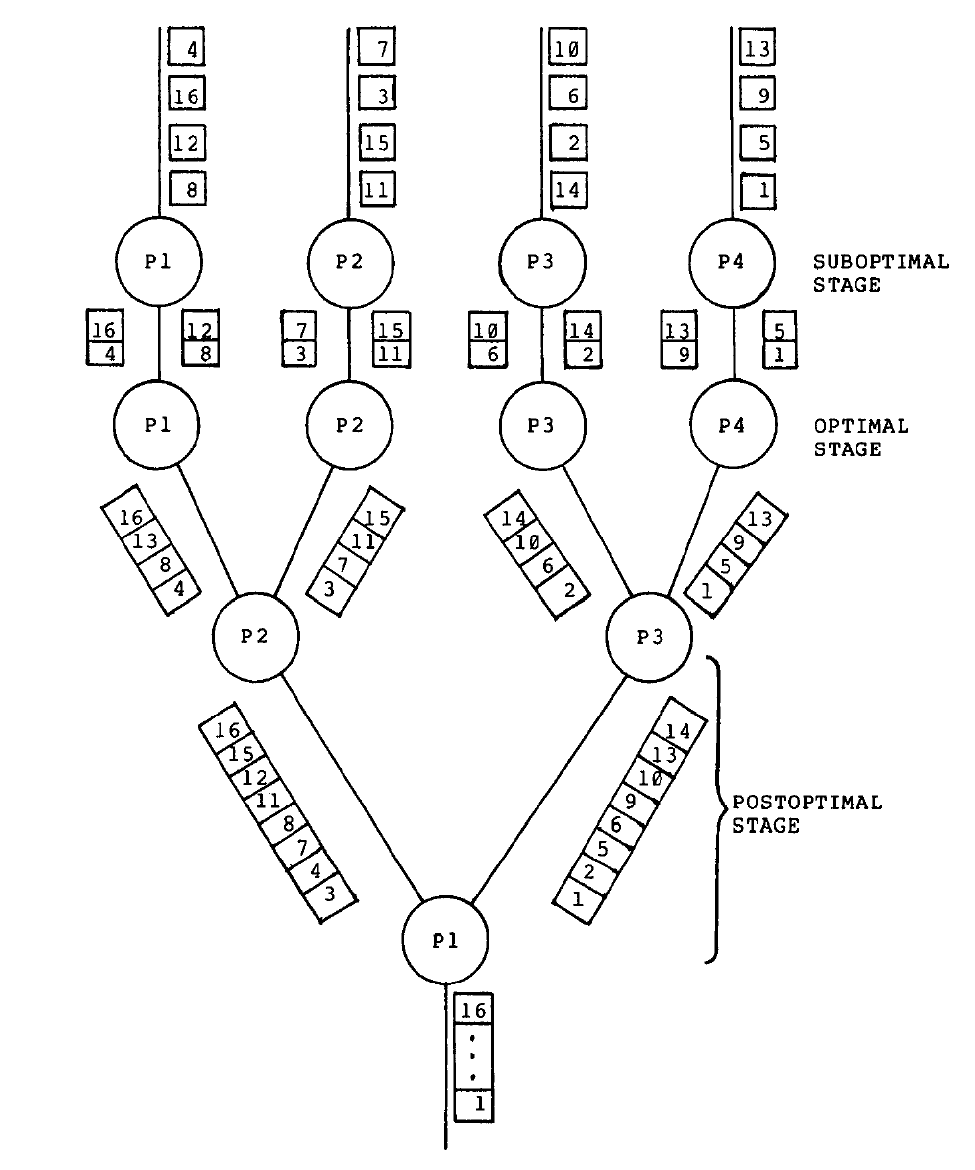
\includegraphics[width=0.5\textwidth]{Bilder/b-merge-sort.png}
	\caption{Paralleler binärer Merge-Sort \autocite[S. 334]{Bitton1983}}
	\label{img:bMergeSort}
\end{figure}

Parallele Merge-All-Sorts \parencite[S. 831f]{Taniar2000} setzen sich aus zwei Phasen zusammen. In einer Sortierphase wird mit einem seriellen internen Sortierverfahren in den einzelnen Threads sortiert. Dem folgend finden die Merge-Schritte statt, wobei nach jedem Schritt weniger Threads benötigt werden, bis der finale Merge-Schritt nur noch von einem Thread ausgeführt wird. Nachteil dieses Verfahrens ist ein sehr umfangreicher letzter Schritt, der nur in einem Prozess stattfinden kann. Im Unterschied dazu teilt der binäre Merge-Sort \parencite[S. 832f]{Taniar2000} die Merge-Phase in eine Pipeline von Merge-Schritten auf, in der je zwei Läufe zusammengefügt werden. Die Idee der parallelen Version eines binären Merge-Sort \parencite[S. 833]{Taniar2000} ist es, dass die Merge-Phase als Strom konzipiert wird und dementsprechend die Kerne auch in dieser Phase deutlich besser ausgenutzt werden. Ein anderer Ansatz ist es, mithilfe einer Range-basierten Aufteilung zwischen intermediären und finalen Merge-Schritten zu gewährleisten, dass in jedem Merge-Schritt gleich viele Kerne genutzt werden. Dagegen reduziert der parallele Merge-All-Sort \parencite[S. 833f]{Taniar2000} die Höhe des Merge-Baumes, indem der Sortierprozess auf zwei Schritte reduziert wird: eine lokale Sortier- und eine finale Merge-Phase. Der parallele verteilende Sort arbeitet nur mit einer beginnenden Range-basierenden Aufteilung und einem abschließenden Sortierschritt. Bei den Sortierverfahren, die eine Range-basierende Aufteilung nutzen, ist das zentrale Problem, in Näherungsverfahren oder genau berechnet den besten Aufteilungsvektor zu finden \parencite{Lu1994, Iyer1989}. Bei unbekannten Relationen bieten sich also eher Verfahren an, die eine zufällige Partitionierung voraussetzen.

Detailliert werde ich \textcite[S. 333ff]{Bitton1983} folgend auf den binären Merge-Sort eingehen, der in drei Phasen abläuft. Die sogenannte suboptimale Phase reduziert die Anzahl der Läufe so lange, bis so viele Läufe vorhanden sind, wie Kerne genutzt werden, also in jedem Thread einer. In der optimalen Phase gibt es für jeden Kern genau einen Lauf und in der postoptimalen Phase wird solange verschmolzen, bis nur noch ein Lauf vorhanden ist. In dieser Phase gibt es zwar weniger Läufe, als Kerne genutzt werden, aber über Pipelining wird trotzdem die Parallelität optimal verwendet, anders als in einigen trivialen Ansätzen {\autocite{Yu1998}}, die kein Pipelining nutzen und so in der postoptimalen Phase in jedem Schritt die Parallelität reduzieren. Die Laufzeit dieses Ansatzes ist wie folgt:

\[ \underbrace{\frac{n}{2p} \log \left( \frac{n}{2p} \right)}_{suboptimal} + \underbrace{\frac{n}{2p}}_{optimal} + \underbrace{\log p - 1 + \frac{n}{2}}_{postoptimal} \]

Allerdings nutzt der bisher beschriebene binäre Merge-Sort den vorhandenen Arbeitsspeicher nicht aus. Deshalb bietet es sich an, die Läufe im Arbeitsspeicher vorzusortieren, um die I/O-Belastung zu reduzieren. Der Fast-Sort-Algorithmus \parencite{Tsukerman1986, Salzberg1990} schlägt hier ein Sortieren über Replacement Selection \parencite[vgl.][]{Knuth1973} vor, da dieses Sortierverfahren längere Läufe erzeugen kann, als in den Hauptspeicher passen würden und eine gleichzeitige Ein- und Ausgabe möglich ist, die das Pipelining optimieren kann. Eine Verteilung auf die anfänglichen Threads findet nach Round-Robin statt.

\textcite{Salzberg1990} betont, dass die Phasen, die die Läufe sortieren, vor allem durch die CPU limitiert sind, aber die Merge-Phasen durch die Geschwindigkeit des Zugriffs auf den permanenten Speicher, da die einzelnen Läufe, sofern größer als der Hauptspeicher, auf Festplatten ausgelagert werden müssen. Dementsprechend lohnt es sich, jedem Lauf eine eigene Festplatte zuzuweisen. \textcite{Hao2009} erläutert die optimale Verwendung des Prozessor-Caches.

\begin{figure}
	\centering
	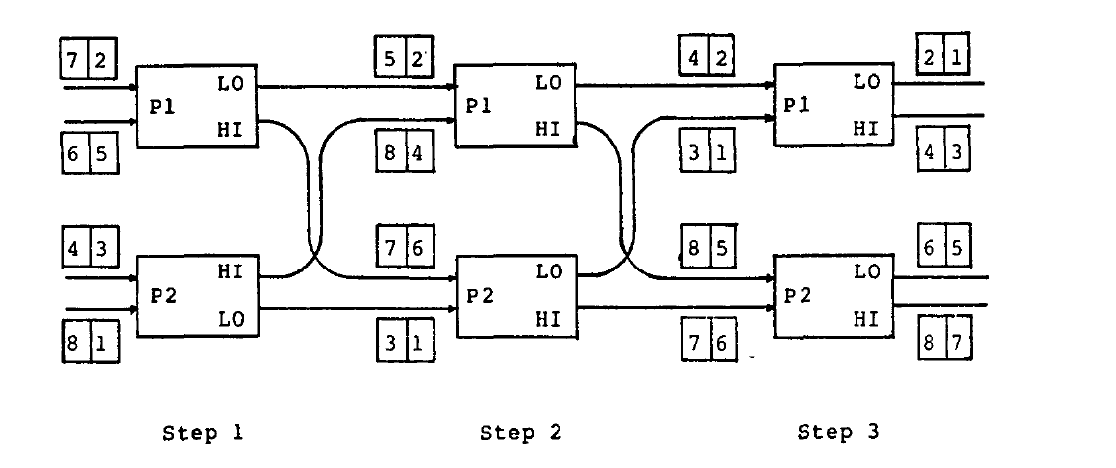
\includegraphics[width=0.75\textwidth]{Bilder/bitonic_block.png}
	\caption{Block Bitonic Sortiernetzwerk mit zwei Prozessoren \autocite[S. 335]{Bitton1983}}
	\label{img:bitonic}
\end{figure}

Das Bitonic-Sortiernetzwerk {\autocite[S. 335f]{Bitton1983}} hat den Vorteil, dass in jedem Schritt die gleiche Anzahl von Kernen genutzt wird. Jeder Schritt besteht aus parallelen Modulen, die Werte vergleichen, in 2 Gruppen aufteilen und dann in einen nächsten Schritt transportieren. Der Algorithmus sortiert $n$ Werte mit $\frac {n} {2} $ Vergleichs-/Austauschmodulen in $\frac{1}{2} \log n (\log n +1)$ Schritten. \autoref{img:bitonic} zeigt Block-Bitonic-Sort mit 2 Modulen. Module können als Prozessoren/Kerne begriffen werden. Verallgemeinert auf einen externen Algorithmus werden in den Modulen die Vergleiche mit einem externen Sortieralgorithmus ausgeführt. Sortiernetzwerke stellen also eine Alternative dar zum Ansatz des Pipelinings. Da der Algorithmus höchstens $2p$ Blöcke sortieren kann, braucht es eine vorbereitende Phase, beispielsweise mit einem parallelen 2-Wege-Merge-Sort, bis die Blockgröße für den finalen Schritt erreicht. Die Gesamtkosten des Bitonic-Sortiertnetzwerkes betragen:

\[ \left[ \log _B (\frac {N} {B P}) + \frac {\log _2 ^2 2 P} {2} + \frac {\log _2 ^2 P} {2} \right] ( \frac {N}{B P}) C _{P} ^{B} \]

{\textcite{Menon1986}} schlägt eine modifizierte Version des Block Bitonic Sort als externen parallelen Algorithmus vor, der Bitonic Sort als internen Algorithmus nutzt und mit Pipelining kombiniert. Pipelining beschleunigt den Merge-Schritt, aber nicht Bitonic Sort selbst. Das interne Sortieren bringt einen Performance-Vorteil gegenüber mehrfachem Verschmelzen. Pipelining lohnt sich vor allem, wenn es eine große Anzahl von Merge-Schritten gibt.

Untersuchungen von {\textcite{Bitton1984}} legen nahe, dass sich für externes Sortieren der parallele binäre Merge-Sort mit Pipelining am besten eignet. Dagegen stellt {\textcite{Menon1986}} fest, dass der binäre Merge-Sort-Algorithmus nur bei großem $n$ und einer kleiner Kernzahl schneller als der Block Bitonic Sort ist.

\subsubsection{Equi-Join} (2 S)
\label{Equi Join} 

Joins gehören zu den teuersten Operatoren in Standard-Datenbanken und sind die einzigen Operatoren, die es erlauben, mehrere Relationen zu verbinden. Dementsprechend werden sie sehr häufig angewandt und die Diskussion um mögliche Performancegewinne durch eine Parallelisierung ist umfangreich {\autocite{Richardson1987, Valduriez1984, Schneider1989, DeWitt1985, Lu1994}}. Die wichtigsten Join-Operatoren sind der Nested-Loop-Join, Sort-Merge-Join, die Gruppe der Hash-Joins und Hash-partionierenden Joins {\autocite{Mishra1992, Lu1994}}, auf deren parallele Implementierung ich im folgenden eingehen werde.

Da sich allgemein Schleifen sehr einfach parallelisieren lassen, liegt für den Nested Loop ein sehr einfacher paralleler Algorithmus vor. Allerdings ist der Nested Loop Join in seiner seriellen Implementierung sehr teuer. Insbesondere wenn die Selektivität gering ist, sind die meisten Vergleiche nicht notwendig. Deswegen lohnt sich der Nested Loop Join auch in einer parallelen Variante nur, wenn entweder ein Full-Outer-Join vorgenommen wird oder fast alle Tupel miteinander verbunden werden. Die Komplexität beträgt $ O(n m) $, also im parallelen Fall $ O( \frac {n m} {p} )$ {\autocite[S. 72]{Mishra1992}}. Im Gegensatz zu den Join-Algorithmen, die Hashing nutzen, ist der Nested-Loop-Join und auch der Sort-Merge-Join in der Lage, Bereichs-Verschmelzungen vorzunehmen, zumindest in der Grundform. 

Der Sort-Merge-Join gehört zu den effizienten Algorithmen in Single Thread-Datenbanksystemen. Die Idee ist es, zuerst beide Relationen, die verschmolzen werden sollen, zu sortieren, um sie dann einfach verbinden zu können {\autocite[S. 149]{Lu1994}}. Wie sich der Sort-Schritt parallelisieren lässt, habe ich bereits erläutert. Allerdings ist es schwer, den Merge-Schritt zu parallelisieren. Sort-Merge-Joins verbessern sich nur schwach mit der Anzahl der Prozessoren {\autocite{Yu1998}}. Ein Ansatz einer weitergehenden Parallelisierung wird mit der Fragment- und Replicate-Methode vorgestellt {\autocite {Richardson1987}}. Die Beiden zu verschmelzenden Tabellen werden partitioniert. Hier gibt es zwei Möglichkeiten: Jede sortierte Partition der Basistabellen aus R wird mit jeder aus S mit Merge-Join verbunden oder die kleinere Relation wird zuerst verschmolzen. Dieser Ansatz ermöglicht eine stärkere Parallelisierung, hat aber Probleme in der Performance, da er eine Annäherung an einen Loop Join darstellt. In einer anderen Methode findet eine Range-Partitionierung in $k$ Fragmente statt. Die entsprechenden Paare können dann verschmolzen werden. \textcite{Iyer1989} schlagen ein Verfahren zur Ermittlung einer idealen Partitionierung vor. Die Sort-Merge-Join-Algorithmen erhalten die Reihenfolge der Relationen und haben Vorteile, wenn Relationen bereits sortiert sind bzw. ein Index vorliegt.

Hash-basierte Join-Algorithmen sind besser geeignet für eine Parallelisierung. Beide Phasen, die Partitionierungs-Phase und die Join-Phase, können parallelisiert werden. Die Grundidee ist es, beide Relationen mithilfe einer Hash-Funktion in Buckets aufzuteilen und nur Tupel zu testen, die in gleichen Buckets sind. Die Komplexität der Grundform beträgt $O(m + n)$, da jede Relation nur einmal gescannt werden muss, sofern die Hashfunktion und die Verteilung ideal ist. Für eine Shared-all-Architektur bietet sich eine globale Hash-Tabelle an. Alle Einprozessor-Hashjoin-Algorithmen können auf diese Art und Weise parallelisiert werden. Probleme können bei ungünstigen Hash-Funktionen mit ungleicher Verteilung und beim Überlauf der Hash-Tabellen auftreten. Auf diese Problematik werde ich später eingehen. Grace- und Hybrid-Hash-Join-Verfahren eignen sich besonders gut für eine Parallelisierung {\autocite{DeWitt1985}}. Eine mögliche Optimierung stellen Bit-Array-Datenstrukturen dar, um zu markieren, dass matchende Tupel existieren {\autocite{Valduriez1984}}.

\begin{itemize}
	\item Simple Hash: Partitioniere weiter auf jedem Kern und speichere nicht behandelte Tuple temporär {\autocite{Lu1994}}.
	\item Grace-Join: Phase 1 + 2: Beide Relationen werden partitioniert. In einer finalen Phase findet das Matching statt. Jeder Behälter muss in den Arbeitsspeicher passen. Der fundamentale Unterschied zu Sort-Merge-Join und Simple Hash-Join ist die zweifache Partitionierung bei der Bucket-Formung und bei der Bucket-Verschmelzung {\autocite{Schneider1989}}.
	\item Hybrid-Join: Versucht I/O-Verkehr zu minimieren, indem beide Phasen des Grace-Joins nicht völlig getrennt sind. In jedem Kern findet eine Join-Phase direkt im Hauptspeicher statt. Drei Phasen: 1) R in n Buckets. Erstes Bucket in-Memory. 2) S in n Buckets. Wieder erstes Bucket direkt im Speicher und testen auf Joins (parallel). 3) Der Rest wird Verschmolzen. Versucht für alle Buckets ein Overflow zu vermeiden. Partitionierung von R überlappt mit Joining im Hauptspeicher {\autocite{Schneider1989}}.
\end{itemize}

Hashtabellen müssen in den Speicher passen, da sonst in der Matching Phase der Join-Operatoren teure I/O-Operationen anfallen. Prinzipiell werden zwei Lösungsansätze diskutiert: Es ist von mehr Partitionen auszugehen als theoretisch notwendig sind, um einer ungleichen Datenverteilung vorzubeugen. Allerdings sind für diesen Ansatz Kenntnisse über die Relationen notwendig und eine sinnvolle Wahl der Anzahl von Partitionen ist nur durch einen Optimierer möglich. {\textcite{Lu1994}} diskutiert, welche Statistiken über die Verteilung innerhalb der Relationen notwendig sind und wie das Load Balancing gestaltet werden soll, also ob eine First-fit- oder Best-fit-Strategie gewählt, aber auch, ob das Load Balancing dynamisch oder statisch vorgenommen werden soll. Ein anderer Ansatz ist das nachträgliche Aufteilen der Hash-Tabellen {\autocite{Mishra1992}}. Das Overflow-Problem der Buckets kann durch einen rekursiven Partitionierungsprozess gelöst werden {\autocite{DeWitt1985}}.

Ein weiterer Faktor für die Performance ist die Task-Generierung, also die Frage, ob Subrelationen überlappend oder vollständig geteilt werden,%Komma weg 
und die Anzahl der erzeugten Tasks. Bei Hash-Joins zum Beispiel stellt sich die Frage, ob für jeden Kern ein Prozess gestartet wird oder nicht. Beim Grace-Join-Algorithmus werden teils mehrere Threads pro Kern verwendet {\autocite{Lu1994}}. 

Hash-partitionierende Joins folgen einem Divide- und Conquer-Ansatz und kombinieren die Idee der Hash-Joins mit der Performance von Sort-Merge-Sorts in ihrer Einkern-Version. Damit wird die Schwierigkeit umgangen, Sort-Merge-Joins zu parallelisieren {\autocite[S. 75ff]{Mishra199}}. Die Idee ist simpel. Beide Relationen werden mit einer Hash-Funktion auf die Threads verteilt. Dem folgend findet in jedem Thread lokal parallel ein Sort-Merge-Join statt {\autocite{Richardson1987}}. Wenn die R-Relation größer ist als der Arbeitsspeicher, gibt es mehrere Läufe {\autocite{Lu1990}}.

In einem detaillierten experimentellen Performance-Vergleich paralleler Join-Implementierungen stellt {\textcite{Valduriez1984}} fest, dass Nested Loop-Joins bei einer sehr hoher Prozessor-Zahl die beste Performance haben, Sort-Merge-Joins bei großen Relationen und Hash-Joins, wenn es eine vergleichsweise geringe Anzahl von Treffern gibt. Zu beachten ist aber, dass hier teils sehr einfache Varianten der Algorithmen verwendet werden. Darüber hinaus haben derzeitige Desktop- oder Server-Prozessoren nicht eine Kernzahl, die mit den Prozessorzahlen damaliger Großrechnersysteme vergleichbar ist. Nach {\textcite{Richardson1987}} haben Hash-basierende Algorithmen die beste Performance unter den parallelen Join-Implementierungen {\autocite[vgl. auch ]{Gerber1986}}. Die Kommunikation zwischen den Clustern ist in einer Shared-Nothinng%Nothing?
-Architektur ein Flaschenhals. Bei normal verteilten Relationen sind Hybrid-Joins als parallele Algorithmen am performantesten {\autocite{Schneider1989}}. {\textcite{DeWitt1985}} schränkt ein, dass ein paralleler Hybrid-Join eine schwächere Festplatten-Nutzung und eine stärkere Prozessornutzung hat als der Grace-Join. Hybrid-Joins profitieren insbesondere davon, dass heutzutage deutlich mehr Hauptspeicher zur Verfügung steht als in den 80ern, als die meisten hier zitierten Performance-Analysen vorgenommen worden sind. Ein grundsätzliches Problem von Hash-Algorithmen ist es, dass diese für eine ungünstige Verteilung von Daten anfällig sind {\autocite{Lakshmi1990}}.

\subsubsection{Spatial Join} (3  S)
\label{Spatial Join} 

Die Berechnung räumlicher Prädikate ist meistens CPU-intensiv. Dementsprechend macht es Sinn, vor einer genauen Berechnung ein mögliches Ergebnis abzuschätzen, um die Anzahl der Join-Kandidaten vor einer exakten Berechnung einschränken zu können. Der Spatial-Join besteht deswegen meist aus zwei Phasen: einer 
Phase, Filter-Schritt genannt, in der ein Set an Kandidaten über eine Abschätzung bestimmt wird, und eine zweite Refinement-Phase, in der die exakte geometrische Berechnung vorgenommen wird {\autocite[S. 309f]{Rigaux2001}}. Eine Parallelisierung findet über eine Partitionierung statt {\autocite{Zhou1998}}. Für den Filter-Schritt 
werden verschiedene räumliche Dekompositionsstrategien angewendet. Der Refinement-Schritt kann separat implementiert werden. Dann ist nur eine Partitionierung über Round Robin notwendig. Wenn der Refinement-Schritt in den Spatial-Join-Operator integriert wird, sind komplexere Strategien der Lastenverteilung möglich {\autocite{Brinkhoff1996}}. Sowohl für die Partitionierung als auch für den Filterschritt wird eine vereinfachte Repräsentation räumlicher Stukturen gewählt, die die Komplexität räumlicher Daten reduziert. Im Allgemeinen wird ein geometrisches Objekt über seine minimale Bounding Box (MBB) genähert, also das minimale Rechteck, welches das geometrische Objekt umschließt {\autocite[S. 202f]{Rigaux2001}}. Allerdings existieren auch andere Ansätze wie z.~B. das True-Hit-Filtering {\autocite{Bouros2019}}.

Eine Parallelisierung basiert auf einer vorherigen Partitionierung. Partitionierungstechniken natürlicher Joins können nicht für Spatial-Joins genutzt werden. Ein in nicht-räumlichen Datenbanken üblicher SASJ-Ansatz (Single Assignment, Single Join) kann hier nicht verwendet werden. Räumliche Paritionierungsmethoden sind entweder Mehrfachzuweisungs-Single-Joins (MASJ) oder Einfachzuweisungs-Mehrfach-Joins (SAMJ), abhängig davon, ob eine MBB mehreren Partitionen zugewiesen wird oder beispielsweise der Mittelpunkt als Repräsentation gewählt wird. Demzufolge können als Join-Kandidaten Duplikate entstehen, die üblicherweise entweder direkt bei der Entstehung entfernt werden oder abschließend an dem Filter-Schritt. Da insbesondere beim Ansatz mit Z-Ordnungs-Quadbäumen eine Duplikatsentfernung sehr aufwändig ist, werden Ansätze diskutiert, die lediglich auf eine Duplikatsvermeidung setzen, aber Duplikate nicht restlos ausschließen {\autocite{Jacox2007, Luo2002}}. 

Eine Partitionierung basiert üblicherweise auf einer räumlichen Dekomposition. R-Bäume werden für SAMJ genutzt, R+-Bäume, Gitter und der Z-Wert für MASJ {\autocite{Zhou1998}}. {\textcite{Brinkhoff1996}} schlägt eine parallele Partitionierung mit R*-Subbäumen und einem globalen Buffer vor. Ein regelmäßiges Gitter als Partitionierungskriterium hat den Nachteil, dass eine Verteilung der Objekte auf die Gitterzellen sehr ungleich sein kann. Als Lösung gibt es mehrere Ansätze: Wenn es deutlich mehr Gitterzellen als spätere Threads gibt, kann durch eine Neuzuweisung einzelner Gitterzellen die Verteilung gleichmäßiger vorgenommen werden {\autocite{Patel1996}}. Auch kann eine Technik, Sort-Tile-Recursive genannt, dafür genutzt werden, ein unregelmäßiges Gitter zu erzeugen, welches eine Gleichverteilung garantiert. Dieses Verfahren wurde ursprünglich für den Bulk-Load von R-Bäumen entwickelt {\autocite{Leutenegger1997}}.

Sowohl für die Partitionierung als auch für den Filter-Schritt werden verschiedene räumliche Datenstrukturen verwendet, die ich einführend kurz erläutere, bevor ich wichtige Ansätze für Spatial-Joins kurz skizziere. Die Z-Ordnung ist ein Ansatz, mehrdimensionale Objekte so mit einem regulären Gitter zu approximieren, dass nahe beieinander liegende Punkte auch in der linearen Ordnung nahe beieinanderliegen. Damit können eindimensionale Baumstrukturen als Index genutzt werden. In der Z-Ordnung wird ein Gitter in der Form aufgebaut und strukturiert, dass das Gitter rekursiv in Quadranten aufgeteilt wird. Diese Quadranten werden mit einem Bitstring codiert in der Reihenfolge eines liegenden Z. Für eine Indexierung wird die Z-Ordnung in Quad-Bäumen eingefügt, in denen nicht die MBBs als Approximation genutzt werden, sondern die Gitterzellen {\autocite[S. 227ff]{Rigaux2001}}.

R-Bäume sind die wichtigste Indexstruktur räumlicher Daten, die Rechtecke in einem Höhen-balancierten Vielwegesuchbaum verwalten. Teilbäume sind nicht zwingend disjunkt. Knoten teilen den Raum in Rechtecke auf und in den Blättern sind die Rechtecke, also im Allgemeinen MBBs, gespeichert. Jeder Knoten außer der Wurzel hat zwischen $m$ und $2 m$ Einträge.

Grundsätzlich reduziert der Filter-Schritt die Relation auf die Kandidaten, deren Approximierungen sich überlappen. Ansätze nutzen entweder eine Indexstruktur über Varianten von R-Bäumen bzw. Z-Ordering-Quadbäume oder verwenden eine Hashing-Stratgie.

Eine Nutzung einer einfachen Gittervariante der Z-Ordnung, in der Objekte durch minimale Quadranten genähert werden, führt zu einer hohen Zahl von Duplikaten. Deswegen schlagen {\textcite[S. 280f]{Rigaux2001}} eine Approximation durch ein festes Gitter vor. Kandidaten werden bestimmt durch parallele Durchläufe der beiden Bäume unter Verwendung eines Sweepline-Scans der z-Achse entlang. Im Anschluss ist es notwendig, nach einer Sortierung der Objekte Duplikate zu entfernen. Nachteil der Nutzung von Z-Ordnungs-Quadbäumen ist ein sehr schlechtes Worstcase-Verhalten mit $n_1 n_2$ mit $n_i$ gleich der Anzahl der Blätter des entsprechenden Baumes und der zusätzliche Aufwand der Duplikatsentfernung, bei der sortiert werden muss und die nicht on-the-fly vorgenommen werden kann {\autocite[S. 284]{Rigaux2001}}. 

Liegen für beide Relationen bereits R-Bäume vo, was häufig der Fall ist, wenn Spatial-Joins direkt auf Relationen in der Datenbank angewandt werden, bietet sich ein synchronisierter traversaler Durchlauf durch beide Bäume an. Wichtiges Kriterium für eine effiziente Implementierung ist die Reduktion von MBB-Schnitttests, die wesentlich teurer als Vergleiche von Standard-Daten sind. Daneben müssen I/O-Zugriffe reduziert werden. Deswegen ist eine simple Umsetzung der traversalen Durchläufe nicht effizient, da sehr viele Rechteck-Schnitttests notwendig sind {\autocite[S. 284f]{Rigaux2001}}. Zwei Ansätze werden vorgeschlagen, die Anzahl notwendiger Tests zu reduzieren: Einerseits kann der Suchraum in jedem Knoten auf den Schnitt mit demselben Knoten im anderen Baum und damit die Zahl der zu testenden Kandidaten reduziert werden. Andererseits kann in den Blättern, die je eine Speicherseite an Objekten beinhalten, ein Sweep-Line-Algorithmus für den Test auf Rechteckschnitte verwendet werden, der in solch einer Form vereinfacht werden kann, dass er kein optimales Verhalten bei einer sehr großen Anzahl von Rechtecken mehr zeigt, da deren Anzahl durch die geringe Größe der Speicherseiten begrenzt ist {\autocite[S. 286f]{Rigaux2001}}. 

Sofern keine Indexe über die räumlichen Attribute vorhanden sind, kann ein Spatial-Hashjoin-Ansatz verfolgt werden {\autocite[S. 288]{Rigaux2001}}. Buckets sind hier Gitterzellen, denen diejenigen MBBs zugeordnet werden, die die entsprechende Zelle schneiden. Offensichtlich kann ein Objekt auch mehreren Gitterzellen zugeordnet werden. Dementsprechend sind unter den Join-Kandidaten Duplikate möglich, die in der Regel dort entfernt werden, wo sie entstehen {\autocite{Zhou1998, Luo2002}}. Die Effizienz des Spatial-Hashjojns hängt von der Wahl der Hashfunktion ab: Es sollte eine gleiche Verteilung der Rechtecke auf die Buckets angestrebt werden, die Buckets sollten in den Hauptspeicher passen und Rechtecke sollten möglichst selten mehreren Buckets zugeordnet werden. Ähnlich wie beim Ansatz mit zwei R-Bäumen kann die Join-Phase eines Buckets z.~B. mithilfe eines Plane-Sweep-Algorithmus beschleunigt werden {\autocite[S. 290]{Rigaux2001}}. Dieser Ansatz ist stark von der Verteilung in beiden Relationen abhängig. Insbesondere ist es problematisch, wenn die zweite Relation eine völlig andere Verteilung hat als die erste.

Ein weiterer Ansatz für einen Spatial Join ohne verherigen Index ist der Index-Nest-Loop-Join {\autocite[S. 10f]{Jacox2007}}, der eine Verbesserung eines Nest-Loop-Joins 
darstellt. Für eine Relation wird ein In-Memory-Suchbaum erzeugt, im Allgemeinen ein R-Baum. Die andere Relation wird gescannt und Join-Kandidaten über den Index gesucht. Wie auch bei den anderen Spatial-Join-Algorithmen ist es notwendig, sich mit Überläufen zu beschäftigen, sofern bestimmte Datenstrukturen für eine performante Ausführung im Hauptspeicher gehalten werden müssen. Hier wäre ein Ansatz denkbar, die nicht indexierte Relation mehrfach mit je einem neuen Teil-R-Baum der indexierten Relation zu scannen. 

Eine Grundidee einer Parallelisierung des Refinementschritts ist simpel. Die Kandidaten können nach Round Robin auf die einzelnen Kerne verteilt werden und die Prädikate über die Queryprozessoren der Datenbanksysteme ausgewertet werden. Allerdings werden in der Literatur viele Ansätze diskutiert, die für spezielle Topologien parallele Ansätze diskutieren {\autocite{Bouros2019, Rigaux2001}} oder über eine Verschränkung des Filter- mit dem Refinementschritt eine bessere Lastenverteilung zu erreichen versuchen {\autocite{Brinkhoff1996, Jacox2007, Zhou1998}}. Wichtig für die Performance dieses Schritts ist es auch zu vermeiden, dass die vollständigen räumlichen Objekte, die Teil diverser Kandidatenpaare sein können, mehrfach in den Hauptspeicher gelesen werden müssen. Sofern nicht ein Ansatz verfolgt wird, der das Refinement mit dem Filterschritt in einem Pipeline-System verbindet, lohnt es sich {\textcite[ S. 45f]{Jacox2007}} folgend, die Kandidatenpaare zu sortieren.

\section{Entwicklung}
3/4 (45 S.)

\subsection{Problemstellung} 3 Seiten
\label{problem}

Im Folgenden werde ich die Entwicklung und Implementierung von drei parallelen Operatoren und einigen Hilfsoperatoren für die MultiThreaded-Algebra kritisch dokumentieren. Anschließend werde ich meine Implementierung experimentell analysieren, indem ich einerseits die einwandfreie Funktionsfähigkeit überprüfen, das Verhalten im Vergleich zu anderen Operatoren und unter unterschiedlichen Rahmenbedingungen betrachten werde. Einwandfreie Funktionsfähigkeit meint Korrektheit, Robustheit und Effizienz im Laufzeitverhalten. Ein Vergleich findet vor allem mit den Einkernversionen der Operatoren statt.

Eine Parallelisierung innerhalb des Datenbanksystems wird hier durch die direkte Implementierung paralleler Operatoren gelöst. Ein anderer Ansatz wäre es, Operatoren zur Verfügung zu stellen, die über den Operatorenbaum sozusagen extern eine parallele Ausführung ermöglichen, entweder durch eine parallelisierte Pipeline oder indem Operatoren für eine Partitionierung von Daten an parallel auszuführende Einkernoperatoren zur Verfügung gestellt werden. Der Nachteil dieses Ansatzes ist, dass keine Anpassungen an den Operatoren mehr vorgenommen werden könnten. Spezielle Optimierungen für eine parallele Ausführung sind also nicht möglich; der Daten- und Kommunikationsfluss orientiert sich ausschließlich an einem Fork-Join-Architekturmuster. Partitionierung und Zusammenführung der Daten können nicht mit der Ausführung verschränkt werden und weder ist eine Kommunikation zwischen den Operatoren möglich noch ein dynamisches Load Balancing. Allerdings hat die Parallelisierung innerhalb von Operatoren auch einen Nachteil: Stehen bei dem externen Ansatz alle Operatoren zur Verfügung, die sich für beide mögliche Ansätze eignen, d.~.h. nicht blockierende Operatoren für eine Pipelineverarbeitung und Operatoren, bei denen nicht zwingend eine Ausführung auf dem gesamten Datensatz notwendig ist, müssen bei dem hier verfolgten Ansatz Operatoren explizit zur Verfügung gestellt werden.  

Damit Operatoren geeignet sind für eine parallele Implementierung müssen sie folgende Kriterien erfüllen. Ziel einer Parallelisierung ist dabei immer ein Laufzeitgewinn.

\begin{itemize}
	\item Berechnungen, die auf verschiedene Prozesse verteilt werden können, müssen eine notwendige Komplexität haben, die den notwendigen Verwaltungsaufwand der Parallelisierung aufwiegt.
	\item Eine Aufteilung von Teilschritten oder -berechnungen auf mehrere Prozesse muss sinnvoll sein.
	\item Der Operator muss üblicherweise große Datenmengen verarbeiten.
	\item Zuerst ist es sinnvoll, Operatoren auszuwählen, die häufig verwendet werden, wobei es hier für unterschiedliche Anwendungsfälle Unterschiede geben kann.
	\item Sofern auch andere Ansätze der Parallelisierung verfolgt werden, ist es insbesondere sinnvoll, Operatoren auszuwählen, bei denen ein externer Ansatz nicht möglich ist.
\end{itemize}

Im Rahmen der \Fb{MThreaded-Algebra} habe ich mich dafür entschieden, je einen Sort-, einen Equi-Join- und einen Spatial-Join-Operator zu entwickeln und zu implementieren. Auch wenn es sicher interessant wäre, verschiedene Algorithmen experimentell zu vergleichen, habe ich für jeden Operator nur einen Ansatz verfolgt, da sonst der zeitliche Rahmen dieser Arbeit gesprengt worden wäre. Einen Vergleich habe ich nur theoretisch vorgenommen, um die konkrete Entscheidung für einen Ansatz zu begründen. Im Folgenden werde ich kurz erläutern, warum ich mich die oben genannten Operatoren gewählt habe:

Ein Sort-Operator (\autoref{Sort}) wird häufig verwendet und ist auch die Grundlage für weitere Operatoren, die eine Sortierung verlangen oder für die Erstellung von Indices. Auch wenn in den meisten Ansätzen der Overhead für eine Parallelisierung recht gering ist, hängen die Kosten für die Vergleiche stark davon ab, nach wie vielen und welchen Attributen sortiert werden soll. Sowohl eine Partitionierung als auch internes Pipelining ist möglich. Da Sortierungen meist für ganze Relationen vorgenommen werden, lohnt sich ein Performancegewinn. Eine externe Parallelisierung wäre lediglich denkbar mit einer Bereichs-Partitionierung, da in diesem Fall sortierte Teildaten wieder zusammengesetzt werden können, wobei eine Bereichs-Partitionierung nur sinnvoll vorgenommen werden kann, sofern Statistiken über die zu sortierende Relation vorliegen. Im Gegensatz dazu ist ein explizit parallel implementierter Sort-Operator auch zu einer Lastenverteilung in der Lage, wenn keine Statistiken über die Relation vorliegen.

Equi-Joins (\autoref{Equi Join}) sind eine der teuersten und am häufigsten angewandten Datenbankoperationen. Da sich darüber hinaus, jenseits des Sort-Merge-Algorithmus, die Ansätze zumindest für einen Equi-Join gut für eine Parallelsierung eignen, ist es sinnvoll, diesen Operator in einer parallelen Variante zur Verfügung zu stellen. Allerdings beruhen die meisten Parallisierungs-Ansätze vor allem auf einer Partitionierung der Daten, die sich schwer dynamisieren lässt. Dementsprechend kann zu dem jetzigen Zeitpunkt nicht gesagt werden, ob eine explizite parallele Implementierung vorteilhaft ist gegenüber eines externen Ansatzes. Dies gilt vor allem für Hash-Joins.

Entgegen der beiden erstgenannten Operatoren hat der Spatial Join (\autoref{Spatial Join}) einen beschränkten Anwendungsbereich im Rahmen von Spezialanwendungen, nämlich geografischen Datenbanken. In diesem Feld ist er eine teure und häufige Operation. Da eine der Stärken von Secondo in seinen Erweiterungen für Nichtstandard-Datenbanktypen liegt, ist es sinnvoll, auch für diesen Bereich eine Parallelisierung zur Verfügung zu stellen. Da in Spatial Joins einerseits häufig große Datenmengen verarbeitet werden und auch die Berechnungen räumlicher Beziehungen teuer sind, lohnt es sich, diesen Operator zu parallelisieren. Es existieren diverse Ansätze zu einer parallelen Implementierung. Ein externer Ansatz ist zwar möglich, aber hat beispielsweise Nachteile im Bereich der Duplikatsvermeidung, da eine Duplikatsentfernung nur als nachfolgender Schritt machbar ist. Auch würde es Query Kenntnisse über Ansätze der Parallelisierung vorraussetzen und die Anfrage selbst wäre zu komplex. 

Da ich hier Operatoren nur für eine shared-all-Architektur (\autoref{P_DBS_DBS}) entwickle, ist es wichtig, insbesondere deren Implikationen zu betrachten. Ein gemeinsam geteilter Permanentspeicher bedeutet, dass I/O-Operationen zum Flaschenhals werden können, da hier keine Parallelisierung möglich ist. Algorithmen müssen also so gewählt werden, dass sie so wenig I/O-intensiv wie möglich sind. Geteilter Speicher dagegen ermöglicht eine vergleichweise kostengünstige Kommunikation zwischen den Prozessen und die Nutzung globaler Strukturen, die von allen Prozessen geteilt werden.

Abschließend fasse ich noch einmal die Ziele für die Implementierung der MThreaded-Algebra zusammen:

\begin{itemize}
	\item Implementierung einer parallelen Version der Operatoren Sort, Equi-Join und Spatial-Join.
	\item Alle entwickelten Operatoren arbeiten mit mindestens drei Kernen: ein Kern für den Hauptprozess und mindestens zwei weitere Threads.
	\item Gleicher Funktionsumfang wie Einkernversionen und einfache Bedienbarkeit.
	\item Alle Operatoren sollen mit beliebig großen Relationen und allen möglichen Attributen arbeiten können.  
	\item Korrektheit, d.~h. unter allen Bedingungen richtige Ergebnisse.
	\item Robustheit, d.~h. keine Abstürze bei Fehleingaben und korrektes Arbeiten auch bei ungewöhnlichen Strukturen/Verteilungen der Eingaberelationen.
	\item Effizienz, d.~h. bessere Performance als Einkernversionen der entsprechenden Operatoren ab einer Mindestrelationsgröße.
	\item Ziel ist hier, dass der Geschwindigkeitsgewinn pro Kern mit vollem Funktionsumfang möglichst linear ist. Zumindest soll versucht werden, den Overhead so gering wie möglich zu halten.
\end{itemize}

\subsection{Entwurf} 10 Seiten
\label{Entwicklung} 

\subsubsection{Operatoren für die Parametrisierung}

Die Parametrisierung der \Fb{MThreaded}-Algebra soll mithilfe von drei Operatoren vorgenommen werden:

\begin{itemize}
	\item maxcore gibt die maximale Anzahl von Kernen/Threads des Systems aus.
	\item setcore setzt die Anzahl der Threads, die von den Operatoren der Algebra genutzt werden. Der Standardwert ist 3.
	\item getcore gibt die Anzahl der Threads aus, die in der Algebra verwendet werden.
\end{itemize}

\subsubsection{k-Merge-Sort} 3 S
\label{entw:sort}

Es soll ein Operator entworfen werden, der eine Relation nach beliebigen Attributen sortieren kann. Der Funktionsumfang entspricht dem Single-Thread-Operator \Fb{sortby} aus der \Fb{ExtRelation2}-Algebra. Sortierkriterien können beliebig viele Attribute der eingehenden Relation sein und für jedes Attribut kann gesondert die Sortierreihenfolge festgelegt werden. Die Relation wird dem Operator als Tupel-Strom übergeben und Ausgabe ist wiederum ein Tupel-Strom. Dabei soll es nicht erforderlich sein, dass die Reihenfolge der Relation erhalten bleibt, sofern Tupel identische Attribute in den Sortierkriterien haben, da dies nach einer zufälligen Partitionierung nur mit großen Aufwand erreicht werden kann.

Zur Auswahl stehen zwei grundsätzliche Ansätze, einen parallelen Sort-Operator zu implementieren: der Block Bitonic Sort und Varianten des Merge Sort. Der Vorteil des Block Bitonic Sort, in jedem, auch dem letzten Schritt alle Kerne gleichmäßig zu nutzen, wird allerdings relativiert. Der Algorithmus muss, sofern die Relation wesentlich mehr Tupel enthält als Kerne zur Verfügung stehen, trotzdem ein externes Sortierverfahren vorschalten. Also ersetzt das Sortiernetzwerk nur die Merge-Phase eines parallelen 2-Wege-Merge-Sorts. Sortiernetzwerke haben auch nur einen Performancevorteil, wenn bei geringer Größe einer Relation viele Kerne zur Verfügung stehen. Deswegen entscheide ich mich, einen 2-Wege-Merge-Sort zu implementieren und zwar in einer Version, die auch im Merge-Schritt die zur Verfügung stehenden Kerne optimal nutzt und die in der Lage ist, eine Vorsortierung auszunutzen und Läufe erzeugen kann, die wesentlich größer sind als Hauptspeicher zur Verfügung steht.

Der von mir gewählte Fastsort-Algorithmus ist ein 2-Wege-Mergesort, in dem Replacement Selection für den Hauptspeicher-Sortierprozess und Pipelining für den Merge-Prozess angewandt wird. Ein paralleler 2-Wege-Mergesort läuft dabei in folgenden drei Phasen ab:

\begin{itemize}
	\item Suboptimale Phase: Erstellung von Läufen mit einem internen Sortierverfahren und einem Merge-Prozess, bis nur noch ein Lauf vorhanden ist. In dieser Phase läuft in jedem Thread ein interner Sortieralgorithmus ab, der identisch mit der Single-Thread-Version ist.
	\item Optimale Phase: Sie ist erreicht, wenn in jedem Thread die Läufe zu genau einem Lauf zusammengefasst worden sind. Die Anzahl der notwendigen Merges entspricht also genau der Zahl der genutzen Kerne. 
	\item Postoptimale Phase: In jedem Schritt finden weniger Merge statt als Kerne genutzt werden. Im letzten Schritt findet nur noch ein Merge statt.
\end{itemize}

Nicht optimal ist in der oben beschriebenen Grundversion eines 2-Wege-Mergesorts die Nutzung der Kerne in der postoptimalen Phase. Deswegen wird hier ein Pipelining für den Merge-Prozess vorgeschlagen. Tupel werden kontinuierlich als Strom weitergereicht, um verschmolzen zu werden bis sie abschließend im Ergebnis in sortierter Reihenfolge entsprechend eines Sortiervektors ausgegeben werden. 

Aus der Sicht der Entwicklung lässt sich der Operator in zwei Phasen unterteilen, die sich in ihrer Struktur deutlich unterscheiden. Als erstes beschreibe ich, wie die suboptimale Phase umgesetzt wird. Dem folgend werden die notwendigen Elemente der postoptimalen Phase beschrieben. Das Scheduling, in dem die Daten verteilt sowie wieder eingesammelt und die Threads verwaltet werden, ist Teil des Secondo-Hauptthreads. Damit entspricht die Architektur des Operators einem Master-Worker-Schema.

Die suboptimale Phase setzt sich aus zwei Schritten zusammen, dem Sortieren und damit Erzeugen von Läufen sowie einem Merge-Prozess, der als Ergebnis genau einen Lauf pro Thread erzeugt. Zuerst werden sortierte Läufe erstellt, bis der Eingangsstrom der entsprechenden Partition erschöpft ist. Als internes Sortierverfahren wird Replacement Selection mithilfe eines Sortierbaums verwendet, um Läufe erzeugen zu können, die deutlich mehr Speicher belegen können, als Hauptspeicher zur Verfügung steht. Als Datenstruktur für das Sortierverfahren wird ein Wettbewerbsbaum verwendet. \autoref{list:fastsortSub} zeigt, wie der Schritt aufgebaut ist, in dem die Läufe erzeugt werden. Der letzte erzeugte Lauf kann im Hauptspeicher gehalten werden. Alle anderen müssen in temporäre Dateien ausgelagert werden. Das bedeutet, dass der Algorithmus auch vollständig im Hauptspeicher ablaufen kann, sofern die Relation inklusive der benötigten Datenstrukturen weniger Speicher belegt als Hauptspeicher zur Verfügung steht. Anschließend werden je zwei Läufe so lange verschmolzen, bis nur noch ein Lauf vorhanden ist, der dann als Eingang für die postoptimale Phase dient. Das Verschmelzen findet statt, wie in  \autoref{list:fastsortMerge} beschrieben.

\begin{minipage}{\linewidth}
	\begin{lstlisting}[caption={Fastsort: Erzeugen der Runs in der Suboptimalen Phase}, label=list:fastsortSub] 
	while (stream and memory) 
		read stream
		fillTree
	endwhile
	while (stream)
		tuple = sortTree->Replace (stream->tuple)
		appendAtRun(tuple)
		if (treeRootIsInactive)
			setTreeAsActive
	endwhile
	saveTreeAsRun
	\end{lstlisting}
\end{minipage}

Die postoptimale Phase hat die Aufgabe, in einer Pipeline von Merge-Schritten die Läufe so lange zu verschmelzen bis ein Ergebnis in einem Ausgangsstrom vorliegt. Wie man in \autoref{img:bMergeSort} sieht, hat die Merge-Pipeline eine Baumstruktur. Die Threads der Merge-Pipeline haben je zwei Eingangsströme und einen Ausgangsstrom. Weitergegeben wird immer der Wert, der entsprechend der definierten Sortierung in der Ausgaberelation vor dem anderen kommt. Der weitergegebene Wert wird aus dem Eingangsstrom ersetzt, aus dem er entnommen worden ist. Es muss zwei grundsätzlich unterschiedliche Typen geben von Merge-Pipeline-Segmenten: Typen mit eventuell persistierten Läufen als Eingang (Blätter des Pipeline-Baums, hier \Fb{MergeFeeder} genannt) oder mit Strömen (Knoten und Wurzel der Pipeline, \Fb{MergePipeline} genannt). Sofern es nicht $2^n$ Blätter gibt, muss es vom ersten Typen von Segmenten auch eine Version geben, die nur aus einem Lauf liest und die Tupel direkt in die Pipeline weitergibt (\Fb{noMergeFeeder}). Alle Merge-Pipeline-Segmente, aber auch der Merge-Prozess innerhalb der suboptimalen Phase funktionieren nach dem gleichem Prinzip, das hier exemplarisch am Beispiel eines Merge an einem Baumknoten dargestellt ist (\autoref{list:fastsortMerge}). Der Merge-Baum benötigt maximal einen Thread weniger als Threads in der suboptimalen Phase vorhanden sind.

\begin{minipage}{\linewidth}
	\begin{lstlisting}[caption={Fastsort: Merge in Pipeline}, label=list:fastsortMerge] 
	while (true)
		if (first/secondTupleEmpty)
			inbuffer1/2->dequeue()
		if (not first/secondTupleEmpty)
			compare(first and second tuple)
			outbuffer->enqueue(smallerTuple)
		else if (first/secondTupleEmpty)
	endwhile
	\end{lstlisting}
\end{minipage}

Das Scheduling, welches im Hauptthread stattfindet, hat drei Aufgaben: die Erzeugung und Verwaltung von Threads und Datenstrukturen für die Datenweitergabe zwischen den Threads, die Partitionierung und Weitergabe des Eingangsstroms des Operators und das Einsammeln des Ergebnisstroms. Für die postoptimale Phase wird eine Pipeline mit einer Baumstruktur, wie oben beschrieben, erzeugt. Sofern zwei Threads damit fertig geworden sind, ihren endgültigen Lauf zu erzeugen, kann die Merge-Pipeline auch schon teilweise gestartet werden. Sinnvoll ist es hier, mit den \Fb{MergeFeedern} zu starten, die Vergleiche vornehmen müssen und zwei Eingangs-Buffer verarbeiten. Genauso ist es sinnvoll, in den langsameren \Fb{MergeFeedern} die Läufe zu verarbeiten, die im Hauptspeicher gehalten werden. \Fb{NoMergeFeeder} dagegen erzeugen nur einen Ausgangsstrom der Länge eines Laufs und kommen ohne Vergleiche aus. Die Ungleichverteilung der Geschwindigkeiten auf verschiedenen Ästen des Baums kann für das Scheduling berücksichtigt werden und verspricht einen Performancevorteil.

Die Datenaufteilung wird nach \Fb{Round-Robin} vorgenommen. Ein Nachteil der Mehrkernversion ist hier, dass Replacement Selection zwar Vorteile hat, wenn Relationen teilweise sortiert sind, aber vorsortierte Teilrelationen auf mehrere Threads verteilt werden, also der Vorteil nicht vollständig zum Tragen kommt. Abschließend können, sofern die ersten beiden Werte im letzten Schritt der Merge-Pipeline prozessiert worden sind, die Ergebnisse bereits an den Ausgabestrom des Operators weitergegeben werden. Eine Ausgabe kann also bereits deutlich vor Abschluss der Operators beginnen.

\subsubsection{Hybrid Hash Join} 3 S
\label{entw:hash}

Der parallele Join-Operator soll zwei beliebig große Relationen verschmelzen anhand je eines Attributs aus beiden Relationen. Der Operator verfügt über keine Statistiken für beide Relationen und soll bei beliebigen Verteilungen gut funktionieren. Orientierung für die Auswahl eines Algorithmus sind dabei Relationen, die nicht in den Hauptspeicher passen und eine gleichmäßige Verteilung beider Relationen bzgl. der Join-Attribute.

In \autoref{Equi Join} habe ich gezeigt, dass für einen parallelen Ansatz vor allem die beiden Hash-Join-Varianten Grace und Hybrid in Frage kommen. Bei verhältnismäßig großem Hauptspeicher und insbesondere in einer shared-all-Architektur schneidet der Hybrid-Hash-Join besser ab. Grund ist vor allem, dass der Hauptspeicher dafür genutzt wird, einen Bucket direkt auf Joins zu testen, und dass die I/O-Kosten des Algorithmus deswegen geringer sind. Da in meiner Implementierung nur eine Festplatte genutzt wird, sind die Kosten für einen Zugriff auf nicht flüchtigen Speicher ein Flaschenhals für die Performance der Implementierung.

\begin{figure}
	\centering
	\subfloat[][]{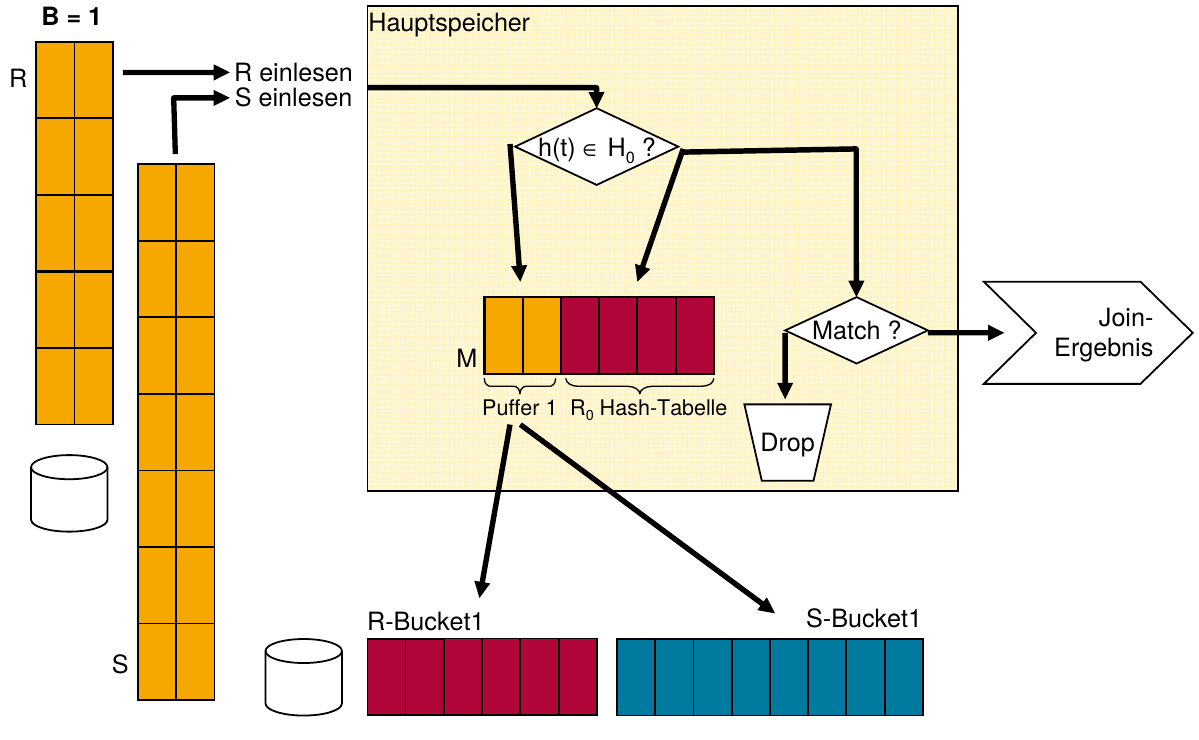
\includegraphics[width=0.4\linewidth]{Bilder/hybrid1.png}}
	\qquad
	\subfloat[][]{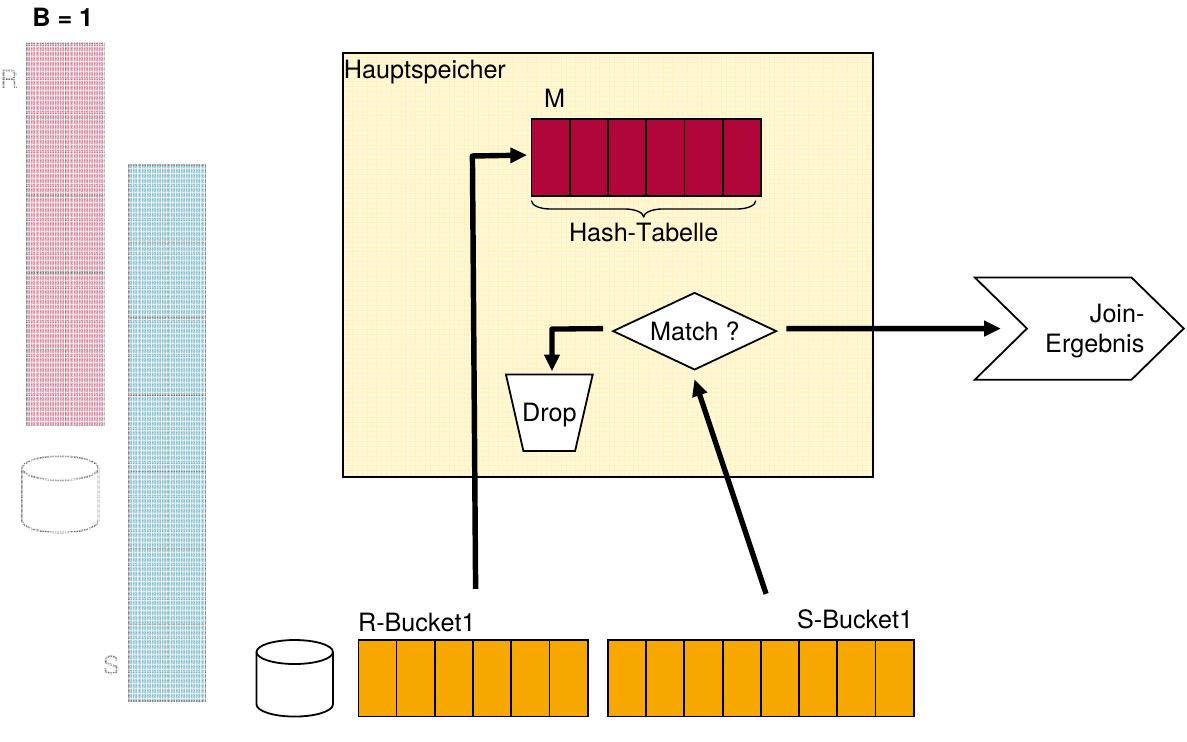
\includegraphics[width=0.4\linewidth]{Bilder/hybrid2.png}}	
	\caption{Hybrid Hash Join in 2 Phasen \autocite{Richly2009}}
	\label{img:hybrid}
\end{figure}

Anders als der parallele Sort-Operator unterscheidet sich der parallele Hybrid-Hash-Join nur durch eine Hash-Partitionierung von der Single Thread-Version. Der Algorithmus, der innerhalb der einzelnen Threads abläuft, ist jeweils ein serieller Hybrid-Hash-Join. In einem ersten Schritt werden also so viele Partitionen erzeugt, wie Kerne verwendet werden und die entsprechenden Tupel als Strom an die Hash-Join-Worker genannten gleichzeitigen Prozesse verteilt.

Der Algorithmus lässt sich in zwei Phasen aufteilen (siehe \autoref{img:hybrid}). In der ersten Phase wird die erste Relation so auf Buckets verteilt, dass ein Bucket möglichst den dem Thread zur Verfügung stehenden Hauptspeicher füllt. In diesem Bucket wird eine Hauptspeicher-Hashtabelle angelegt, in der idealerweise in jedem derer Buckets genau ein Tupel gespeichert wird, um die Anzahl notwendiger Vergleiche so gering wie möglich zu halten. Hier sieht man bereits, dass die Verteilung der Relation für die Effizienz dieses Algorithmus von großer Bedeutung ist. Die anderen Buckets werden temporär zwischengespeichert. In einem zweiten Schritt wird die zweite Relation durchgescannt und vergleichbar verfahren: Tupel, die dem ersten Bucket zugeordnet werden, können direkt an den Ergebnisstrom weitergegeben werden, wenn sie in den Join-Attributen mit dem Tupel der ersten Relation übereinstimmen. Die anderen Buckets werden wie bei der ersten Relation temporär zwischengespeichert. \autoref{list:hybrid} zeigt den Ablauf der ersten Phase. Da zum Abschluss dieser Phase beide Relationen einmal durchgelaufen sind, können Statistiken ermittelt werden, die es in der zweiten Phase ermöglichen, anstatt mit vorher festgelegten Werten für die Anzahl der Buckets mit abgeschätzen zu arbeiten. Auch wenn dies nicht vollständig verhindern kann, dass einzelne Hashtabellen nicht in den Hauptspeicher passen, ist es doch ein wichtiger Ansatz, um die Chance möglicher Overflows zu reduzieren.   

\begin{minipage}{\linewidth}
	\begin{lstlisting}[caption={Phase 1 Hybrid Hash Join}, label=list:hybrid] 
	readNextTupleR
	while (StreamR) 
	bucket = calculateBucket
	if (bucket = 0)
	if (overflow)
	overflowhandling
	insertInMemoryHashTable
	elseif
	insertInPersistentHashStructur
	readNextTupleR
	endwhile
	
	readNextTupleS
	while (streamS)
	bucket = calculateBucket
	if ()bucket = 0)
	if (overflowR)
	overflowhandling
	for (allInSameInMemoryHashBucket)
	if (equalOnJoinAttr)
	result = concat(tupleR, tupleS)
	insert result in resultBuffer
	elseif
	insertInPersistentHashStructur
	readNextTupleS
	endwhile
	\end{lstlisting}
\end{minipage}

In der zweiten Phase werden dann die restlichen Buckets der ersten Aufteilung der Reihe nach in den Hauptspeicher geladen und in der gleichen Art und Weise Tupel bestimmt, die in ihren Join-Attributen übereinstimmen. Da jetzt bereits bekannt ist, ob die einzelnen Buckets in den Hauptseicher passen, müssen nicht mehr, wie in Phase 1, bei einem Überlauf Teile eines Buckets in eine Überlaufstruktur geschrieben werden, sondern diese kann direkt angelegt werden.

Der Umgang mit möglichen Overflows macht den Algorithmus deutlich komplexer als eine Version, in der unendlich viel Hauptspeicher zur Verfügung stünde. Auch wenn in vielen Fällen Hash-Join-Algorithmen sehr effizient sind, haben sie ein schlechtes Worst-Case-Verhalten, da in einem Extremfall alle Tupel den gleichen Hash-Wert hätten. Danit der Algorithmus auch für ungünstig verteilte Relationen funktioniert, wird die Overflow-Behandlung rekursiv angelegt. Die Grundstruktur des Algorithmus bleibt dabei dieselbe, aber in jedem Durchlauf kann erneut ein Overflow auftreten. Da dies das gute Verhalten des Hybrid-Hash-Joins bzgl. der I/O-Kosten umkehrt, ist es sehr wichtig, im ersten Scan einer Relation Statistiken über diese zu generieren, die die Hash-Funktion so optimiert, dass möglichst keine Overflows auftreten.

\subsubsection{Spatial Join} 3 S

Aufgrund einer besseren Vergleichbarkeit mit den bereits in Secondo vorhandenen Operatoren habe ich den Spatial Join auf zwei Operatoren aufgeteilt, nämlich einen Filter-Schritt (\Fb{MThreadSpatialJoin}) \footnote{Die Bezeichnung ist hier etwas verwirrend. Der Filter-Schritt ist nicht der spätere Filteroperator, sondern der Refinement-Schritt.} und einen Refinement-Schritt (\Fb{MThreadFilter}), auch wenn ein Performance-Vorteil zu erwarten ist, wenn beide Operatoren in einem Operator zusammengefasst werden, da einerseits eine Weitergabe des Tuple-Stroms über eine Schnittstelle des Secondo-Kerns entfällt und die Möglichkeit eines dynamischen Load-Balancing besteht. Ein weiterer Vorteil der Trennung ist, dass ein separater Filter-Operator für den Refinement-Schritt universell nutzbar ist.

Hier soll ein universell nutzbarer Spatial-Join-Operator implementiert werden. Dementsprechend muss bei der Entscheidung für einen Algorithmus beachtet werden, dass dieser keine spezifischen Voraussetzungen hat. Weder wird davon ausgegangen, dass Indices noch Statistiken über die Relation vorliegen. Also kommen vor allem zwei Algorithmen infrage: der Spatial-Hash-Join oder ein interativer Spatial-Join mit einem R-Baum. Auch wenn in der Literatur für den hier vorliegenden Kontext häufig Spatial-Hash-Joins empfohlen werden, haben diese zwei Nachteile. Bei unbekannten Relationen ist es schwer, ein optimales Gitter zu bestimmen. Gibt es zu viele Gitterzellen, werden viele Duplikate erzeugt, die auch jedes Mal erneut auf die Joinbedingung getestet werden müssen;  gibt es zu wenig Gitterzellen, liegen viele Objekte in der gleichen Gitterzelle. Verschärft wird das Problem noch dadurch, dass ein Spatial-Hash sehr anfällig gegenüber ungünstigen Verteilungen ist. Deswegen entscheide ich mich hier, einen internen R-Baum zu erzeugen und die zweite Relation seriell zu durchlaufen. Für den Fall, dass die Relation, über die ein R-Baum erzeugt wird, nicht in den Hauptspeicher passt, muss dieser Prozess mehrfach wiederholt werden. Deswegen wird von einem iterativen Spatial-R-Baum-Join gesprochen.

Um den Operator zu parallelisieren ist es notwendig, beide Relationen zu partitionieren. Da hier deutlich weniger Gitterzellen notwendig sind als für den Join-Prozess, bietet sich eine Gitter-Partitionierung an. Um zu vermeiden, dass die Verteilung auf die Gitterzellen sehr ungleichmäßig wird, wähle ich hier ein irreguläres Gitter, welches mit der Sort-Tile-Recursiv-Technik (STR) erzeugt wird. Ein mit STR erzeugtes Gitter stellt sicher, dass die Gitterzellen gleich viele Objekte beinhalten. Um hier den Rechenaufwand zu reduzieren, wird das Gitter nur aus einer Zufallsstichprobe erzeugt, deren Größe mit der Relation wächst. Da dann nicht sichergestellt werden kann, dass alle Objekte im Gitter liegen, ist das Gitter an den Rändern offen. Ein anderer sinnvoller Ansatz der Partitionierung wäre es, über Zweige eines R-Baums zu partitionieren. Der Vorteil wäre, dass der erste Scan der R-Relation während der Partitionierungsphase bereits für den Aufbau der Datenstruktur für den Join-Prozess genutzt werden könnte. Der R-Baum würde dann allerdings nicht parallel erzeugt werden. Ich habe mich gegen einen globalen R-Baum entschieden, um einerseits auch diesen Schritt parallelisieren zu können und da andererseits die Eliminierung von Duplikaten in einer Gitterstruktur nicht so rechenaufwändig ist.

Anders als bei den beiden anderen implementierten Operatoren ist es nicht nur eine Frage der Performance, ob der Algorithmus gegenüber einer Single-Thread-Variante modifiziert wird. Ein prinzipieller Unterschied einer parallelen Implementierung ist, dass räumliche Objekte, sofern sie eine Ausdehnung haben, mehreren Gitterzellen und damit Partitionen gleichzeitig zugewiesen werden. Dementsprechend können im Filter-Schritt gleiche Join-Kandidaten in unterschiedlichen Threads doppelt ermittelt werden. Im Anschluss Duplikate zu ermitteln ist sehr rechenaufwändig. Wird lediglich der Kandidat weitergegeben dessen Schnittmenge in der Gitterzelle liegt, die sich so weit wie möglich rechts-oben befindet, werden Duplikate bereits in der Entstehung ausgeschlossen.

TODO Bild

Die Beschreibung des Filterschritts beginne ich mit dem Scheduling, in dem das SRT-Gitter für die Partitionierung konstruiert wird, die Worker-Threads erzeugt werden, die beiden Relationen $R$ und $S$ auf die Partitionen verteilt werden und abschließend der Ergebnisstrom an den folgenden Operator weitergegeben wird.

In den Worker-Threads werden zuerst die Tupelströme aus den Partitionen der R-Relation in einen internen R-Baum eingelesen. Der Speicher wird hier global für alle Threads gemeinsam verwaltet. Tupel, die nicht mehr in den Hauptspeicher passen, werden in eine temporäre Datei geschrieben. In einem ersten Schritt wird die S-Relation einmal gescannt und Join-Kandidaten bestimmt sowie auf Duplikate geprüft.  Sofern es einen Overflow gab, kann die Anzahl der Iterationen jetzt genau berechnet werden, da die R-Relation einmal durchgescannt wurde und Statistiken über sie bestimmt werden konnten. In jeder Iteration wird die S-Relation wiederum vollständig durchlaufen und die R-Relation muss inklusive der für den Join notwendigen Datenstrukturen in der Hauptspeicher passen.

\begin{minipage}{\linewidth}
	\begin{lstlisting}[caption={Spatial Join: Worker}, label=list:spatialJoin]
	tupleR = readFromBufferR 
	while (tupleR != nullptr)
	if (globalMemFree)
	putInRTree(tupleR)
	recalcGlobalMemFree
	elseif
	putInOverflowBuffer(tupleR)
	endwhile
	tupleS = readFromBufferS
	while (tupleS)
	calcResult(tupleS,RTree)
	if (noDuplicate)
	putInResult
	tupleS = readFromBufferS
	endwhile
	\end{lstlisting}
\end{minipage}

Auch wenn hier ein sehr großer Performance-Vorteil zu erwarten ist, da die Berechnungen räumlicher Beziehungen bei komplexen räumlichen Objekten sehr rechenintensiv ist, ist die Grundidee des Filter-Operators sehr einfach. Anstatt einen genau auf die Bedürfnisse zugeschnittenen Operator für das Refinement zu implementieren, habe ich mich hier entschieden, einen allgemeinen, universell einsetzbaren Filteroperator für diesen zweiten Schritt des Spatial Joins einzusetzen. Der Tuplestrom wird nach Round Robin auf die einzelnen Threads verteilt, die nur die Tupel zurückgeben, die das Filterprädikat erfüllen.

\subsection{Implementierung} 15 S/ 2 S
\label{Implemeniterung} 

Im folgenden wird die Implementierung der in \autoref{Entwicklung} skizzierten Operatoren und Datenstrukturen, die von den Operatoren gemeinsam genutzt werden, dargestellt. Einleitend werde ich einerseits die genutzte Entwicklungsumgebung skizzieren und andererseits wichtige Ansätze in der Implementierung erläutern, die von übergreifender Bedeutung für die gesamte Implementierung sind.

Die von mir implementierte Algebra wird auf einem OpenSuse Leap 15.0 Linux-System in Secondo 4.20 integriert. Als IDE wurde C-Lion verwendet. Für meine Implementierung musste ich ausschließlich eine Algebra im Secondo-Kern in C++ integrieren und einige Änderungen im Kern und in anderen Algebren vornehmen. Genutzt wurde der C++11-Standard. Vor allem habe ich die ab diesem Standard in die Standard-Library integrierte Concurrency-Bibliothek und \Fb{shared\_pointer} verwendet.

Mit C++11 wurde die Concurrency-Implementierung der Boost-Library in die Standardbibliothek übernommen, die ich in meiner Implementierung verwende. Sie basiert auf dem C++-Speichermodell, der sequentiellen Konsistenz. Es muss also ein deterministisches Verhalten auch eines Programmflusses garantiert werden, der auf mehreren gleichzeitigen Prozessen beruht. Kern der C++-Concurrency-Schnittstelle sind Threads, die ihre ausführbare Einheit enthalten und sofort gestartet werden. Ich verwenden durchgehend Funktionsobjekte, das heißt Instanzen von Klassen, für die der Klammer-Operator überladen worden ist. Der erzeugende Thread kann entweder mit \Fb{join} darauf warten, dass der Thread seine Aufgaben beendet oder den Thread mit \Fb{detach} vom Erzeuger-Thread lösen, mit dem Risiko von undefiniertem Verhalten, da die Existenz gemeinsame genutzer Resssourcen so nicht mehr garantiert ist. Sperren können in Mutexe verpackt werden, von denen ich zwei mit unterschiedlichen Kosten und Funktionen verwende: den \Fb{lock\_guard}, der lediglich sicherstellt, dass die Sperren wieder freigegeben werden und der \Fb{unique\_lock} mit erweiterter Funktionalität. Für meine Implementierung wichtig ist die Möglichkeit, die Sperre pausieren zu lassen, also Sperren mehrfach zu setzen und wieder freizugeben. Mithilfe von Bedingungsvariablen (\Fb{condition\_variable}) kann auf einer Nachricht an einen oder alle Threads gewartet werden. Anzuraten ist es, um Nebeneffekte zu vermeiden, ein Prädikat in Form einer Lambda-Funktion zu verwenden. \Fb{Std::atomic} stellt darüber hinaus atomare Datentypen zur Verfügung, von denen ich Booleans verwende {\autocite{Grimm2018}}. 

\begin{minipage}{\linewidth}
	\begin{lstlisting}[caption={Flags der MThreaded-Algebra}, label=list:flags]
	DEFAULTCCFLAGS += -pthread -DTHREAD_SAFE
	CCFLAGS += -pthread -DTHREAD_SAFE
	COMMON_LD_FLAGS += -lboost_thread -lboost_system
	\end{lstlisting}
\end{minipage}

Eine Schwierigkeit meiner Implementierung ist es, dass ich zwar in der von mir entworfenen Algebra die sequentielle Konsistenz garantieren kann, aber diese an diversen Stellen auf anderen Funktionalitäten des Secondo-Kerns beruht. Probleme traten vor allem im Umgang mit \Fb{FLOBs} auf. Secondo verwendet die Berkeley-DB in einer Konfiguration, die keinen konkurrierenden Zugriff auf die Datenbank-Speicherschnittstelle erlaubt. Deswegen muss sichergestellt werden, dass Zugriffe auf diese nur sequentiell stattfinden. Zuerst gab es Probleme mit der Thread-Sicherheit des FLOB-Managers. Über ein Flag lässt sich Secondo in einem Thread-sicheren Modus kompilieren (siehe \autoref{list:flags}). Vor allem wird bei Verwendung dieses Flags der Flob-Manager synchronisiert. Leider gab es in meiner Algebra weiterhin Probleme mit der Threadsicherheit, sofern direkt auf \Fb{FLOBs} innerhalb von Threads zugegriffen wird. Vor allem tritt dieses Problem bei der Verwendung von Query-Prozessoren innerhalb der Threads im Filter-Operator auf und sofern Attribute in den beiden anderen Operatoren \Fb{FLOBs} sind. Im Detail werde ich das Problem und geeignete Lösungsversuche im \autoref{impl:refinement} diskutieren.

Abhängigkeiten bestehen zu folgenden Algebren, die mithilfe des Makefiles der Algebra eingebunden werden:

\begin{itemize}
	\item StandardAlgebra
	\item StreamAlgebra
	\item RelationAlgebra
	\item SpatialAlgebra
	\item RectangleAlgebra
	\item SPartAlgebra (irreguläres Gitter)
\end{itemize}

Die Schnittstelle für die Integration neuer Operatoren ist genau definiert. Prinzipiell besteht ein Operator aus vier Methoden und zwei weiteren Bestandteilen: Das Typemapping stellt sicher, dass der Operator nur mit Parametern aufgerufen wird, mit denen er funktioniert. Das Valuemapping berechnet aus einer Eingabe das Ergebnis. Die Methode \Fb{getOperatorSec} enthält die Spezifikation des Operators als Text. Die Methode \Fb{getOperator} fasst die Bestandteile des Operators für den Algebramananger zusammen. Zusätzlich notwendig ist eine Datei mit mindestens einem Beispiel für jeden Operator, mit der das Funktionieren der Algebren automatisch überprüft werden kann, und eine Datei, die die Signatur der Operatoren enthält. Alle von mir implementierten Operatoren außer den Hilfsoperatoren, auf die ich hier nicht genauer eingehe, da sie sehr simpel strukturiert sind, haben als Eingangs- und Ergebniswert einen Tupelstrom. Hier ist es notwendig, den Zustand des Operators in einer weiteren Klasse zu erhalten, die LocalInfo-Klasse genannt wird, die in meiner Implementierung die Funktion des Schedulings übernimmt, also Daten verteilt, das Ergebnis weitergibt, die notwendigen Datenstrukturen erzeugt und die Threads erzeugt sowie verwaltet. Zwei Parameter werden für einige Operatoren gesetzt. \Fb{SetUsesMemory} erlaubt es einem Operator, seinen Speicher selbst zu verwalten und ist notwendig bei Operatoren, die größere Datenstrukturen im Hauptspeicher aufbauen. \Fb{SetUsesArgsInTypeMapping} erlaubt den Zugriff auf die Parameter im Typemapping. Ein wichtiger Mechanismus des Type-Mappings, der hier genutzt wird, ist der Append-Mechanismus, der die Weitergabe von dort generierten Informationen an das Valuemapping erlaubt.

Grundsätzlich verwende ich Headerdateien, damit die Schnittstellen einfacher erfasst werden können. Die Implementierungen der Operatoren sind in Ordnern zusammengefasst nach Hilfsoperatoren, Sortieroperatoren und Joinoperatoren. Hilfsstrukturen, die von mehreren Operatoren genutzt werden und darüber hinaus für weitere Algebren zur Verfügung gestellt werden sollen, sind in \Fb{MThreadedAux} zusammengefasst.

\subsubsection{Hilfsstrukturen} 2 S
\label{Hilfsstrukturen} 

In diesem Kapitel stelle ich  selbst implementierte Datenstrukturen vor, die nicht speziell einem Operator zugeordnet werden können, sondern von mehreren Operatoren genutzt werden. Die Operatoren-übergreifend genutzten Datenstrukturen sind in der Datei \Fb{methreatedAux} zusammengefasst. Ich habe drei unterschiedliche Tupelbuffer implementiert und zwei threadsichere Wrapperklassen um die Warteschlange der Standard-Library. Unterschiede zwischen verschiedenen Versionen ist die Fähigkeit, Tupel zwischenzuspeichern.

Tupelbuffer sind für Anwendungsfälle gedacht, bei denen der Schreib- und der Lesevorgang voneinander getrennt ist -- im Allgemeinen wird zuerst eine bestimmte Menge von Tupeln temporär gespeichert, um später wieder vollständig geladen zu werden. Da bei der Initialisierung oft nicht klar ist, ob der Buffer im Hauptspeicher gehalten werden kann oder nicht, gibt es eine virtuelle Bufferklasse, von der ihre Versionen mit gleicher Schnittstelle abgeleitet sind: ein Hauptspeicherbuffer, ein persistenter Buffer und ein Buffer, der intern die Persistierung verwaltet. Intern verwenden die Tupelbuffer, sofern es sich um die Hauptspeicherversionen handelt, als Datenstruktur Warteschlangen und sofern es sich um persistente Buffer handelt, einen Zeiger auf \Fb{TupleFiles} der \Fb{RelationAlgebra}. In disem Fall wird dessen \Fb{MakeScan}-Iterator für den Zugriff auf die Daten verwendet. Zuerst habe ich die temporären Speicher selbst mit \Fb{fileStreams} und der Methode \Fb{WriteToBin} der Tupel-Klasse implementiert, aber mit diesem Ansatz gab es, sofern \Fb{FLOBs} verwendet wurden, Synchronisierungsprobleme. Die Buffer haben eine Read-, eine Append-Methode, Methoden zum Öffnen sowie Schließen und zur Abfrage, ob der Buffer leer ist. In der Hauptspeicherversion des Buffers sind einige Methoden ohne Funktion, waren aber notwendig, damit alle Versionen mit einem gleichen Interface benutzt werden können. Sowohl die persistenten Buffer als auch die Warteschlangen wurden so konstruiert, dass Dateien nicht direkt im Konstruktor angelegt werden, sondern erst, wenn der erste Schreibvorgang notwendig wurde, um zu verhindern, dass, sofern keine Persistierung erfolgte, aber die Datenstruktur bereits erzeugt werden musste, I/O-Operationen durch die Anlage einer Datei notwendig werden.

Die Warteschlange der Standard-Library ist nicht threadsicher. Verwendung finden Warteschlangen vor allem als Buffer für den Datenaustausch zwischen Threads, zwischen denen Tupelströme fließen. Eine persistente Version wurde notwendig, da die Join-Operatoren teils blockieren und bereits deutlich früher einen Ergebnisstrom produzieren als begonnen wird diesen auszulesen. Die nicht persistente Version ist generisch und damit nicht nur für Tupel nutzbar. Für die Synchronisierung wird ein Mutex verwendet und die Dequeue-Methode gibt diesen temporär wieder frei, wenn die Warteschlange leer ist, um in diesem Fall einen Schreibvorgang zu ermöglichen (\autoref{list:queue}). Die persistente Version wird mit dem zur Verfügung stehenden Hauptspeicher parametrisiert und lagert ab dem Zeitpunkt, wenn kein Speicher mehr zur Verfügung steht, die Tupel in ein Fb{TupleFile} aus. Eine Verbesserungsmöglichkeit wäre es, wenn anschließend wieder Hauptspeicher frei werden würde, diesen auch zu verwenden.

\begin{minipage}{\linewidth}
	\begin{lstlisting}[caption={Enqueue und Dequeue-Methode der threadsichere Warteschlange}, label=list:queue]
	void enqueue(T t) {
		std::lock_guard<std::mutex> lock(m);
		q.push(t);
		dataReadyQueue = true;
		c.notify_one();
	}
	
	T dequeue() {
		std::unique_lock<std::mutex> lock(m);
		while (q.empty()) {
			c.wait(lock, [&] { return dataReadyQueue; });
			dataReadyQueue = false;
		}
		T val = q.front();
		q.pop();
		return val;
	}
	\end{lstlisting}
\end{minipage}

\subsubsection{Operatoren für die Parametrisierung}

Die Hilfsoperatoren für die Parametrisierung haben folgende Signaturen:

\begin{itemize}
	\item maxcore: $\longrightarrow int$
	\item setcore: $int \longrightarrow bool$
	\item getcore: $\longrightarrow int$.
\end{itemize}

Die Anzahl der genutzten Kerne wird in einem Singleton in einer statischen Variablen gespeichert. Die Anzahl der maximal nutzbaren Kerne wird über eine Methode der Concurrency-Library ermittelt.

\subsubsection{2-Wege-Merge-Sort} 3 S

Der Operator \Fb{mThreadedMergeSort} hat die Signatur $stream~x~(attr~x~bool \ldots) \longrightarrow stream$. In die Algebra muss er mit zwei Optionen integriert werden: Er muss seinen Speicher selbst verwalten, um zu wissen, wie viel Arbeitsspeicher für die Sortierung der Läufe zur Verfügung steht, und er benötigt seine Argumente im Typemapping, um die Sortierrichtung auswerten und weitergeben zu können. Das Typemapping hat zwei Funktionen: Einerseits muss es sicherstellen, dass die zu sortierende Relation als Tupelstrom in den Operator eingeht und die Sortierattribute Elemente der Tupel sind. Andererseits wird der Append-Mechanismus genutzt, um die Indices der Sortierattribute und die Sortierrichtung an das Value-Mapping weiterzugeben. Die Attribute und die Sortierrichtung werden dem Operator als Liste übergeben, um zu ermöglichen, dass beliebig viele Sortierattribute genutzt werden können, wobei die Richtung als Boolean übergeben werden kann. Wenn keine Richtung explizit gewählt ist, wird sie als aufsteigend gesetzt. Der Operator bricht nur ab, wenn 

\begin{figure}
	\centering
	\includegraphics[width=0.75\textwidth]{Bilder/mergeSort.png}
	\caption{Aufbau des Mergesort-Operators (vereinfacht). Gestrichelte Pfeile: Datenfluss; durchgezogene: Instanzen werden erzeugt}
	\label{img:KlassSort}
\end{figure}


Das Value-Mapping startet lediglich die LocalInfo-Class mit den Suchindices sowie dem verfügbarem Arbeitsspeicher als Argument und holt den sortierten Tupelstrom aus der Pipeline-Instanz, die die Wurzel des Merge-Baums darstellt, über dessen GetNext-Methode ab. Die LocalInfo-Class ist verantwortlich für das Scheduling, Destributor-Collector genannt, das heißt, für die Erzeugung der notwendigen Buffer, der Threads und das Verteilen des eingehenden Stroms auf die Threads. Als Buffer für die Läufe werden die in \autoref{Hilfsstrukturen} dargestellten, selbst implementierten Klassen verwendet, die Daten sowohl im Speicher halten, als auch in eine temporäre Datei auslagern können. Für den Tupelstrom innerhalb der Merge-Pipeline und für die vollständig sortierte Relation wird eine Wrapper-Klasse um die Warteschlange der Standardbibliothek benutzt, die threadsicher gemacht wurde. Vergleiche werden über eine Compare-Klasse vorgenommen, die mit dem Sortiervektor initialisiert wird.

Die Partitionierung wird über an die Thread-Klassen weitergegebenen Iteratoren vorgenommen und eine Synchronisation mit Mutexen und Nachrichten, die mitteilen, in welchem Thread wieder ein Tupel benötigt wird. Anschließend wird die Merge-Pipeline erzeugt aus den Elementen Merge-Feeder, NoMerge-Feeder und Merge-Pipeline. Hier werden die Threads vom Hauptthread entkoppelt, um einen nicht-blockierenden Operator zu ermöglichen, also nach dem Start der Merge-Pipeline sofort die ausgegebenen Tupel über die GetNext-Methode abholen zu können. Im Gegensatz dazu hat es zu undefiniertem Verhalten geführt, auch in der suboptimalen Phase die Threads zu entkoppeln. Der Vorteil einer Entkopplung wäre es, dass, sofern einige Threads der suboptimalen Phase deutlich schneller sind als andere zum Beispiel aufgrund einer teilweisen Vorsortierung, bereits frühzeitig Teile der Merge-Pipeline hätten gestartet werden können. So lässt sich die Laufzeit der unterschiedlichen Äste der Merge-Pipeline nur noch darüber regulieren, dass die Läufe, die im Hauptspeicher gehalten werden konnten, in die aufwändigeren \Fb{MergeFeeder} eingehen.

Wie bereits in \autoref{Entwicklung} dargelegt, läuft die suboptimale Phase in zwei Schritten ab, nämlich der Erzeugung von sortierten Läufen und der Reduktion der Läufe auf genau einen durch mehrere Merge-Phasen. Der erste Schritt wiederum ist in drei Phasen aufgeteilt: In der ersten Phase werden die Blätter des Wettlaufbaums gefüllt und kontinuierlich überwacht, ob noch genügend Speicher vorhanden ist. Der Arbeitsspeicher wird gleichmäßig zwischen den Threads aufgeteilt. Ein Abbruchkriterium für das Füllen des Baums ist, wenn der Speicher durch einen vollständig konstruierten Baum sowie die Speicherrepräsentation der Tupel ausgelastet ist. Im Baum selbst werden nur Pointer gespeichert. Ein zweites Abbruchkriterium ist, wenn der Tupelstrom erschöpft ist, gekennzeichnet durch die Weitergabe eines Nullpointers. Dem folgend wird der vollständige Baum von den Blättern ausgehend konstruiert.

Weitere Läufe zu erzeugen ist nur notwendig, wenn der Tupelstrom noch nicht erschöpft ist, da im anderen Fall bereits genau ein sortierter Lauf erzeugt worden ist, der auch nicht persistiert werden muss. Diese weiteren Läufe werden dadurch erzeugt, dass das aktuelle Tupel des Eingangsstroms mit der Wurzel des Baums ausgetauscht wird und dieser neue Wert weiter in den Baum einsickert. Aus den ausgetauschten Tupeln werden die weiteren Läufe erzeugt, die immer in persistenten Buffern gespeichert werden. Ein neuer Lauf wird angelegt, wenn der aktuelle Wert nicht mehr in den Baum einsickern kann, das heißt, wenn die Wurzel inaktiv ist (die genaue Funktionsweise dieses Sortierbaums werde ich im nächsten Abschnitt erläutern). Abschließend wird der vollständige letzte (oder einzige) Baum in einen speicherinternen Buffer geschrieben.

Der Wettbewerbsbaum ist eine Datenstruktur, die eine Sortierung vergleichbar mit einem Turnierbaum abbildet. Der Baum wird in einem Vektor gespeichert. In jedem Knoten ist je der Nachfolgeknoten mit dem kleineren und größeren Wert durch den Vektorindex, ein Schalter aktiv/inaktiv und ein Zeiger auf den Tupel gespeichert. Blätter sind dadurch gekennzeichnet, dass als Nachfolgeknoten der größte mögliche vorzeichenlose Integer-Wert eingetragen wird. Als inaktiv werden Tupel gekennzeichnet, die erst in der Erzeugung des nächsten Laufs verwendet werden, da sie für den aktuellen Sortierlauf je nach Sortierrichtung zu groß oder zu klein sind. Ein Baum kann keine weiteren Tupel mehr aufnehmen, wenn die Wurzel inaktiv geworden ist. Wenn der Baum noch Werte im aktuellen Lauf aufnehmen kann, wandern Tupel mithilfe einer rekursiven Methode von der Wurzel zu den Blättern und strukturieren den Baum dabei um. Für einen neuen Lauf muss der Baum lediglich wieder vollständig auf aktiv gesetzt werden. 

Der Merge-Schritt entspricht der in \autoref{Entwicklung} beschriebenen Vorgehensweise. In einer Schleife werden je zwei Läufe miteinander verschnitten, bis nur noch ein Lauf übrigbleibt. In der postoptimalen Phase verlaufen die Verschmelzungen vom Prinzip her genauso, aber es wird mit einem Tupelstrom gearbeitet, der durch eine Merge-Pipeline fließt, um die zur Verfügung stehenden Kerne optimal ausnutzen zu können. \Fb{Feeder} haben als Eingang die in der suboptimalen Phase erzeugten Läufe und geben sie entweder einfach weiter (\Fb{NoMergeFeeder}) oder verschmelzen sie vorher (\Fb{MergeFeeder}). Diese Unterscheidung ist notwendig, wenn der Baum der Merge-Pipeline kein vollständig gefüllter Baum ist. Der Pipeline-Schritt, der die Wurzel darstellt, gibt seine Ausgabe an den Buffer aus, der von der \Fb{GetNext}-Methode der \Fb{LocalInfo}-Klasse eingelesen wird. In der Pipeline werden Buffer verwendet anstatt lediglich Tupel weitergegeben, um sicherzustellen, dass es nicht zu einer Blockierung kommt, wenn Verarbeitungsgeschwindigkeiten auf unterschiedlichen Ästen verschieden sind. Die Buffer sind \Fb{shared\_pointer} auf die selbst implementierte threadsichere Queue.  


\subsubsection{Hybrid Hash Join} 3 S
\label{impl:hybrid}

Der Operator \Fb{mThreadedMergeSort} hat folgende Signatur:

$stream~x~(attr~x~bool \ldots) \longrightarrow stream$

In die Algebra muss er mit einer Option integriert werden: Er muss seinen Speicher selbst verwalten, um zu wissen, wie viel Arbeitsspeicher für die Hash-Tabellen zur Verfügung steht. Das Typemapping hat zwei Funktionen. Einerseits muss es sicherstellen, dass die beiden Relationen, die über einen Equi-Join verbunden werden sollen, als Tupelstrom in den Operator eingehen und die Joinattribute Elemente der jeweiligen Tupel sind. Andererseits wird der Append-Mechanismus genutzt, um die Indices der Joinattribute an das Valuemapping weiterzugeben.

Wieder wird das grundsätzliche Entwurfsmuster gewählt, welches in Secondo für Operatoren verwendet wird, die einen Tupelstrom als Ein- und Ausgabe haben. Der Zustand des Operators wird in einer LocalInfo-Class gesichert, auch wenn ein kontinuierlicher Tupelstrom fließt. Hier hat diese Klasse noch die zusätzliche Aufgabe, innerhalb eines Master-Worker-Schemas die Funktion des Masters zu übernehmen: Sie erzeugt die Worker-Threads, partioniert und verteilt die Daten über eine Modulo-Hash-Funktion auf genau so viele Threads wie Kerne genutzt werden und sammelt den Ergebnis-Tupelstrom abschließend wieder über ihre GetNext-Methode ein. Als Buffer wird ein Vektor mit Shared-Pointern auf eine von mir implementierte threadsichere Queue verwendet. In diese Buffer werden nacheinander die beiden eingehenden Relationen verteilt und die Threads vom Hauptthread getrennt, damit ein nicht blockierender Operator ermöglicht wird, da nicht auf die Worker gewartet werden muss, bis Werte von der GetNext-Methode weitergereicht werden können. Da hier keine gleichmäßige Partitionierung stattfindet, wird eine Warteschlange als Buffer gewählt, um Performanceverluste zu vermeiden, wenn ein einzelner Worker auf Daten aus dem Tupelstrom warten müsste.

Die Worker setzen sich aus zwei Klassen zusammen. Eine eigentliche Worker-Klasse, in der die beiden Phasen (\autoref{entw:hash} des Hybrid-Hash-Joins ablaufen, und eine HashTablePersist genannte Klasse, die die Buckets verwaltet, die nicht direkt On-the-fly verschmolzen werden. Insgesamt wird jede Partition auf 20 Buckets aufgeteilt und der erste direkt verschmolzen. Der Wert muss so gewählt werden, dass es wahrscheinlich ist, dass jedes Bucket in den Hauptspeicher passt. Nur aus der R-Relation werden Hash-Tabellen erzeugt -- die S-Relation wird wie die R-Relation in 20 Buckets aufgeteilt, dann aber sequentiell durchlaufen und auf das Join-Kriterium gegenüber der Tupel, die sich im gleichen Bucket der Hash-Tabelle befinden, getestet. In einem Bucket befinden sich als Anfangswert wiederum 1000 Buckets, deren Zahl aber nach einem ersten vollständigen Durchlauf durch beide Relationen neu kalkuliert wird und in der Variable hashmod gespeichert wird. Ziel ist hier, dass möglichst nur ein Tupel in einem Bucket ist. Im Speicher werden die Buckets als Vektor eines Vektors von Zeigern auf Tupel gehalten. In der HashTablePersist-Klasse wird zuerst davon ausgegangen, dass alle Hash-Tabellen aus der R-Relation und auch alle entsprechenden Buffer der S-Relation in den Speicher passen. Der Buffer ist so angelegt, dass der Vektor, der die Buffer speichert, sowohl speicherinterne Buffer aufnehmen kann als auch persistierte. Wenn festgestellt wird, dass nicht genug Hauptspeicher für alle Buffer vorhanden ist, werden zuerst die der S-Relationen weggeschrieben und dann einer nach dem anderen die der R-Relation.

Für die Verwaltung der Threads und die Synchronisierung sind für den Join-Operator lediglich zwei globale Variablen notwendig. Es führte zu undefiniertem Verhalten, wenn die notwendigen Tupel-Vergleiche gleichzeitig stattfindet. Deswegen wird der Aufruf der Compare-Methode von Attribute über einen Mutex abgesichert. Zuerst habe ich auch die Buffer für den Austausch zwischen Worker und Master als globale Variablen realisiert. Da es hier aber Probleme beim Commit gab -- es existierten noch Zeiger auf Relationen, vermutlich temporäre --, habe ich die Buffer über \Fb{shared\_pointer} übergeben. Als Kennzeichen dafür, dass der Ergebnisstrom in der threadsichereren Warteschlange vollständig ist, wird ein Nullpointer genutzt. Da erst der Worker, der als letztes fertig wird, den Nullpointer setzten darf, wird die Anzahl fertiger Threads in einer globalen Variable gezählt.
 
Im Grunde ist die Struktur des Operators sehr simpel. Probleme treten auf zwei Ebenen auf. Bereits erläutert wurde, wie die Anzahl der Buckets in der Hashtabelle nachjustiert wurde. Komplexer ist das Overflow-Problem. Eine Hashtabelle muss, damit der Operator effizient ist, in den Hauptspeicher passen. Jedes mal, wenn eine Hash-Tabelle aus der R-Relation eingelesen wird und festgestellt wird, dass diese nicht in den Hauptspeicher passt, wird die halbe Hash-Tabelle in einen Overflow-Buffer geschrieben. Leider ist es nicht möglich, beim ersten Durchlauf durch die Relation innerhalb der HashTablePersist-Klasse bereits die Overflow-Buffer zu erzeugen, da im Falle eines Overflow die Buffer bereits in einen temporäres File geschrieben worden sind und dementsprechend ohne eine Sortierung vorliegen. Die Overflow-Buffer werden dann in einer rekursiven Methode verarbeitet, damit der Operator auch mit sehr gleichverteilten Relationen zurecht kommt. Nur in so einem Fall sind mehrere rekursive Durchläufe durch den Overflow-Buffer zu erwarten. Grundsätzlich ist diese Anfälligkeit gegenüber der Verteilung der Relationen einer der großen Nachteile des Hash-Joins, der zu einem schlechten Worst-Case-Verhalten führt.

\subsubsection{Spatial Join Filter Step} 3 S

Der Operator \Fb{mThreadedSpatialJoin} hat folgende Signatur:

$stream~x~stream x attr x attr x real \longrightarrow stream$

In die Algebra muss er lediglich mit einer Option integriert werden: Er muss seinen Speicher selbst verwalten, um zu wissen, wie viel Arbeitsspeicher für die internen R-Bäume zur Verfügung steht. Sein Type-Mapping hat zwei Funktionen. Einerseits muss es sicherstellen, dass die beiden Relationen, die verschmolzen werden sollen, als Tupelstrom in den Operator eingehen und die Join-Attribute Elememte der jeweiligen Tupel und von einem räumlichen Datentyp sind. Der fünfte Parameter muss ein Real sein und stellt den Wert da, um den die Bounding Box vergrößert werden kann, um Spatial Joins zu ermöglichen, bei den die Objekte, die im späteren Refinement-Schritt mitels einer Prädikats geprüft werden, einen Abstand zueinander haben. Nearest Neighbour wäre ein Beispiel hierfür. Andererseits wird der Append-Mechanismus genutzt, um die Indices der Joinattribute an das Valuemapping weiterzugeben.

Wie die anderen Operatoren auch, gliedert sich der Operator in zwei zentrale Bestandteile: ein Scheduling, welches von einer LocalInfo-Klasse ausgeführt wird, und Threads als Worker, in denen der Ergebnisstrom berechnet wird. Anders als bei den bisherigen Operatoren kann eine räumliche Partitionierung nicht sinnvoll ohne Kenntnisse über die R-Relation vorgenommen werden. Hier wird die R-Relation einmal gescannt und ein Sample ihrer MBBs erzeugt. Um ein gleichverteiltes Sampling zu erzeugen, werden zunächst die ersten 100 MBBs gespeichert. Anschließend wird eine Zufallszahl erzeugt, die beginnend mit 100 in jedem Durchgang um 1 erhöht wird. Werte zwischen 0 und 99 ersetzen die entsprechende MBB. Um die Größe des Samples an die Größe der Relation anzupassen, wird nach dem Scan von je 1000 Tupeln die Menge der gespeicherten MBBs um 10 erhöht. Nur aus diesen MBBs wird das Gitter mittels STR erzeugt. Hierfür wird die Klasse IrregularGrid2D aus der SPart-Algebra verwendet. Ursprünglich hatte diese nur eine Schnittstelle für Ströme. Für die Anwendung innerhalb dieses Operators habe ich in der Algebra eine Schnittstelle ergänzt, die einen Vektor von Rechtecken als Parameter erlaubt, um eine direkte Parametrisierung ohne Query-Prozessor zu ermöglichen. Da das irrgeguläre Gitter nur aus einer Zufallsauswahl erzeugt wurde, kann es sein, dass räumliche Objekte außerhalb des Gitters liegen. Deswegen wird das Gitter in alle Richtungen bis zu den maximal bzw. minimal möglichen Double-Werten erweitert. Da von einer kleinen Kernzahl ausgegangen wird, erzeuge ich für die Partitionierung ein Gitter, welches aus Streifen besteht, um unproblematisch auch mit einer Anzahl von Threads umgehen zu können, deren Wurzel keine natürliche Zahl ist. Ein Gitter mit mehr Zellen ist nicht anzustreben, da auch mehr Duplikate möglich sind.

Die MBBs werden über ein Funktionsobjekt realisiert, um die Fallentscheidung zwischen vergrößerten und nicht vergrößerten MBBs nur einmal implementieren zu müssen. Die R-Relation muss, da sie bereits im Scheduling gescannt wurde, temporär gespeichert werden. Hierfür wurde ein Buffer implementiert, der seine Persistierung selbst verwaltet (\autoref{Hilfsstrukturen}. Für die interne Speicherung steht der maximale Speicher zur Verfügung. Für die Tupelströme stehen zwei Versionen von Warteschlangen zur Verfügung. Die eingehenden Ströme werden sofort verarbeitet, weswegen die Standardversion der threadsicheren Warteschleife verwendet werden kann. Da aber mehrere Iterationen über die S-Relation notwendig werden können, wenn die R-Bäume inklusive der Repräsentation der Tupel der R-Relation nicht in den Hauptspeicher passen, kann es sein, dass Ergebnistupel zwischengespeichert werden müssen, bevor sie von der GetNext-Methode der LocalInfo-Klasse abgeholt werden können. Hier hilft es auch nicht, die Workerthreads vom Hauptthread zu entkoppeln, da die GetNext-Methode erst Tupel abholen kann, wenn beide Eingangsrelationen vollständig gelesen worden sind. Eine Möglichkeit, dies zu verhinden, wäre es, jedes mal, wenn der Hauptspeicher vollständig belegt ist, zwischen Scheduling und GetNext zu wechseln. Da dies aber nur kompliziert umzusetzen ist, wurde der Ansatz gewählt, der es ermöglicht, den Ergebnisstrom zu persistieren. Für die Datenstrukturen der Worker, vor allem die R-Bäume und Tupelspeicher, wird der Speicherplatz global verwaltet. TODO: Verteilung Speicher, auch noch mal testen. Auch wenn der Speicher global verwaltet wird, habe ich mich gegen einen globalen R-Baum entscheiden, da ich bei einer geringen Anzahl genutzter Kerne von wenigen Duplikaten ausgehe und es deswegen als Vorteil sehe, trotz einer gewissen Redundanz zwischen den R-Bäumen, die Teil-R-Bäume parallel erzeugen zu können.

Der Join-Prozess selbst ist nicht kompliziert. Aus dem Tupelstrom der R-Relation wird ein interner R-Baum aufgebaut, der 4 bis 8 Rechtecke in jedem Knoten aufnehmen kann. Anschließend wird die S-Relation vollständig durchlaufen und Joinkandidaten über eine Suche der MBBs im R-Baum festgestellt. Sofern die R-Relation inklusive des R-Baums nicht mehr in den Hauptspeicher passt, wird der Vorgang wiederholt. Nach einem ersten Durchlauf kann berechnet werden, wie viele Iterationen notwendig sind, wobei immer der maximale Speicherbedarf eines R-Baums vorausgesetzt wird (in der Methode \Fb{calcIterations} wird die Iterationszahl so lange hochgezählt, bis bei der Aufteilung kein Overflow mehr entsteht). Im ersten Durchlauf ist es durchgehend notwendig, den Speicherbedarf zu überwachen, um festzustellen, ab wann die R-Relation nicht mehr in den internen R-Baum geschrieben werden kann, sondern in eine externe Datenstruktur geschrieben werden muss. Die Berechnung des Speicherbedarfs ist komplizierter als bei den anderen Operatoren, da der Speicherverbrauch des R-Baums nicht linear wächst. Allerdings stellt die genutzte Implementierung eines internen R-Baums von Secondo hierfür eine Methode zur Verfügung.

Duplikate machen auf zwei Ebenen Probleme. Einerseits soll das Ergebnis frei von Duplikaten sein. In \autoref{entw:spatial} habe ich bereits erläutert, dass diese in der Entstehung erkannt werden können über ihre Position innerhalb der Gitterzelle, also erst gar nicht als Joinkandidaten an den Ergebnisstrom weitergegeben werden. Für diesen Zweck habe ich die Methoden \Fb{topright} und \Fb{reportTopright} implementiert. Andererseits bereiten Duplikate Probleme bei der Löschung von Tupeln, die keine Joinkandidaten sind. Anders als bei den beiden anderen Operatoren dürfen Tupel erst gelöscht werden, wenn sie in allen Gitterzellen, in denen sie vorkommen, getestet wurden. Für diesen Zweck muss hier der Referenzzähler der Tupel-Klasse genutzt werden, um sicherzustellen, dass ein Tupel erst gelöscht wird, wenn keine Referenz mehr vorhanden ist.

\subsubsection{Spatial Join Refinement Step} 3 S
\label{impl:refinement}

Der MThreadFilter-Operator ist analog des nicht parallelen Filter-Operators angelegt und ist damit vielseitiger zu verwenden als ausschließlich für den Refinement Step eines Spatial Joins. Übergeben wird eine beliebige Funktion. Die Signatur des Operators ist $stream~x~fun \longrightarrow stream$. Auch wenn die Architektur des Operators simpel ist, hat die Implementierung große Schwierigkeiten bereitet und konnte nicht zufriedenstellend gelöst werden. Vor allem liegt das an Problemen mit der Threadsicherheit von \Fb{FLOBs}.

Bereits das Typemmapping ist kompliziert, da anders als in der Single-Thread-Version die übergebende Funktion nicht direkt im Queryprozessor genutzt werden kann, sondern für jeden Thread ein eigener Operatorenbaum für einen eigenen Queryprozessor konstruiert werden muss. Für diesen Zweck ist es notwendig, dass die Argumente, das heißt in diesem Fall die Funktion, an das Typemapping übergeben werden muss. Also wird für den Operator das Parameter \Fb{SetUsesArgsInTypeMapping} gesetzt. Die Attribute der Funktion werden darauf getestet, ob sie im Eingangsstrom vorkommen und das Ergebnis des Prädikats vom Typ Boolean ist. Die Funktion wird als Textobjekt (\Fb{FText}) mithilfe des Append-Mechanismus an das Valuemapping übergeben. Im Scheduling kann die Funktion dann von einem Textobjekt in eine ListExpr umgewandelt werden, um die jeweiligen Operatorenbäume für die Threads zu erzeugen.

Die Implementierung hat mehrere Ziele: Die möglichst vollständige Berechnung, ob Join-Kandidaten auch bei einer genauen Auswertung der Prädikate mit den räumlichen Attributen weiterhin verschmolzen werden müssen oder allgemein, ob die Filter-Prädikate als wahr ausgewertet werden, soll in den Threads vorgenommen werden, da dieser Schritt sehr hohe Kosten verursacht. Eine Synchronisierung gerade der teuren Berechnung soll vermieden werden. Der Operator soll nicht blockierend sein, das heißt es sollen direkt von Filter durchgelassene Tupel an den Ergebnisstrom übergeben werden ohne eine temporäre Speicherung. Darüber hinaus sollen die Threads möglichst nicht pausieren, dass heißt Ein- und Ausgabestrom sollen parallel zur Berechnung der Filterprädikate in den Threads verarbeitet werden.

Durch diese Ziele wird die konkrekte Implementierung des Operators deutlich komplexer als die Single-Thread-Version, da mehrere Threads durchgehend einen Eingabestrom haben müssen und gleichzeitig der Ergebnisstrom weitergeleitet werden muss. Ein trivialer Ansatz, der Tupel an alle Threads verteilt und dann auf die Ergebnisse wartet, um diese weiterzuleiten, kann dazu führen, dass einzelne Threads zwischenzeitlich nicht ausgelastet sind, wenn die Objekte, die in die Berechnung eingehen, sich deutlich in der Komplexität unterscheiden. Mein erster Ansatz versuchte, die Verteilung nach Round Robin in einen eigenen Thread auzulagern, damit Verteilung und Ergebnisweitergabe über die \Fb{getNext}-Methode parallel und damit beide kontinuierlich laufen können. Dieser Ansatz, der voraussetzt, dass die Threads vom Hauptthread entkoppelt werden, ist allerdings schwierig in der Synchronisation vor allem bei der Destruktion von Objekten und führte zu undefiniertem Verhalten vor Allem bzgl. des Schließen des Eingangsstroms und der Zerstörung der Queryprozessoren. Auch trat bereits ein Problem auf, welches ich leider nicht vollständig lösen konnte: Vermutlich durch eine fehlende Synchronisation von nicht zulässigen gleichzeitigen Zugriffen auf die Berkelely-DB-Schnittstelle wurde ein Commit verhindert, da entweder offene Zeiger auf Objekten der Queryprozessoren vorhanden waren oder im Commit noch Sperren bestanden, die teils zu einer Ausnahme führen, teils zu einem Deadlock während des Commits.

Eine erste Vereinfachung versuchte noch die Parallelität von Strömen und Prädikatsberechnungen aufrechtzuerhalten, aber die Probleme zu reduzieren, die dadurch entstanden, wenn der Eingangsstrom in einem eigenen Thread behandelt wird und der Aufruf der Destruktoren der Threads schwer zu koordinieren ist. Jetzt alternierte der Hauptthread zwischen einer Partitionierungs- und der GetNext-Methode. Da nicht vorauszusehen ist, wie groß die Selektivität des Filters ist, musste die GetNext-Methode so implementiert werden, dass sie nur so lange auf Ergebnisse wartet, bis die Buffer, die als threadsichere Warteschlange implementiert sind, fast leer sind. Eine weitere Synchronisation wurde notwendig, um einen Deadlock zu verhindern, wenn der Eingangsstrom erschöpft ist. Zuerst wurden die Queryprozessoren, die die Filterprädikate in den Threads auswerten, auch in diesen erzeugt, was zu Nebeneffekten führte, wenn diese zerstört wurden. Deswegen wurden die Queryprozessoren in der LocalInfo-Klasse erzeugt und in deren Destruktor zerstört. Mit diesem Ansatz gelang es, Probleme auf den Commit zu reduzieren, wenn eine große Relation mit \Fb{FLOBs} verarbeitet wurde.

Eine genaue Lokalisierung des Fehlers ist schwierig, da er sich erst im Commit, also nach Abschluss des vollständigen Querybaums, manifestiert. Der implementierte Operator selbst läuft vollständig mit dem richtigen Ergebnis durch. Der Fehler tritt auch bei nur einem Thread auf, also ist es wahrscheinlich kein Synchronisationsproblem zwischen den Prädikatauswertungen. Eine Vermutung ist es, dass neben den Queryprozessoren der Threads teils Prozesse außerhalb der Threads auch auf \Fb{FLOBs} der Tupelattribute, die in das Prädikat eingehen, zugreifen. Für diesen Zweck war ein weiterer Versucht, einen Performanceverlust in Kauf zu nehmen, indem entweder nur die Prädikatauswertung oder nur die Verarbeitung des Tupelstroms ablaufen darf. Eine Synchronisation wurde mithilfe einer Bedingungsvariable und Mutexen vorgenommen, führte aber auch nicht zu einer fehlerfreien Funktionsweise des Operators. Auch ein letzter Versuch, Secondo ohne Commit zu verwenden, führte zwar dazu, dass deutlich seltener und erst bei größeren Relationen Fehler auftraten, aber immer noch kam es im Abschluss der Abfrage, die den Filter beinhaltete, gelegentlich zu Abbrüchen.

Ein letzter Versuch war es, den Query-Prozessor direkt in den Worker-Threads mehrmals zu erzeugen und wieder zu zerstören. Dieser Ansatz hätte, wenn dies nicht allzu häufig vorgenommen werden muss, zu einem Operator führen können, der zwar nicht optimal Parallelität ausnutzt, aber trotzdem schneller ist als die Single-Thread-Version, sofern die Auswertung der Prädikate entsprechend teuer ist. Die Idee begründet sich darin, dass es erst bei relativ großen Relationen zu dem Commit-Fehler kommt. Allerdings funktionierte dieser Ansatz nur, wenn maximal 20 Tuple ausgewertet wurden, bevor der Query-Prozessor zerstört und wieder neu aufgebaut wird. Damit ist der Operator als parallele Version deutlich langsamer als der Single-Thread-Filteroperator. 

TODO: Frage ob sortieren sinnvoll damit flob nicht mehrmals gelesen
In der RequestProgress Funktion wird z.B. ein "static Word result " benutzt, das bei mehreren Thread problematisch sein könnte. 
Auch ein globales OpNodeAddr2Id ist sich
mutexe in flobmanager
writetobin, jetzt tuplefile

\subsubsection{Probleme mit FLOBs im Multithreading-Secondo}

In diesem Abschnitt versuche ich die Probleme zusammenzufassen, die es mit \Fb{FLOBs} gibt und Ansätze für die Lösung 

\section{Test und Experimente} 15 
\label{te}

Im folgenden Abschnitt werden umfangreiche Tests der Operatoren beschrieben und ihr verhalten unter unterschiedlichen Bedingungen untersucht. Da hier kein abstraktes Laufzeitverhalten betrachtet wird, sondern die konkrete Laufzeit der Implementierung auf einem spezifischen System, beschreibe ich dieses kurz, um die Meßergebnisse kontextualisieren zu können. Da eine Effizienz unter anderem durch einen Vergleich mit Single-Thread-Operatoren festgestellt wird, geht es aber nicht vor allem um Messwerte, sondern um eine Effizienzsteigerung. Dementsprechend geht es vor allem um eine Laufzeitverbesserung unter gleichen Bedingungen und nicht so sehr um das einzelne Messergebnis.

Entwickelt wurde auf einem openSuse Leap 15.0 System mit einem AMD 6300 FX Prozessor (L1-Cache: je Kern 16 KB Daten \& je Modul 64 KB Instruktionen, L2-Cache je Modul 2048 KB mit Prozessortakt, L3-Cache 8 MB mit Northbridge-Takt, 3,5/3,8/4,1 GHz), 16 GB Arbeitsspeicher und einer SSD. Anzumerken ist, dass der Prozessor zwar über
6 Integer-Cluster verfügt, aber nur über 3 Gleitkomma-Einheiten. 2 Kerne sind je zu einem Modul zusammengefasst.

Vergleichend teste ich auch auf einem Windows 2016 Server mit deutlich besserer und aktuellerer Hardware, auf dem Ubuntu 20.04 LS als Gast-Betriebssystem unter VMWare Workstation Player läuft. Der Server hat 2x Xeon Gold 6128 mit je 6 Kernen (L1: 384 KB, L2 6 MB, L3 19,25 MB, 3,7/3,54 GHz), 396 GB Arbeitsspeicher und zwei SSDs. Dem Gast-Betriebssystem stehen insgesamt 10 Kerne zur Verfügung und 32 GB Arbeitsspeicher. Vorteil hier ist neben dem modernen Mehrkernsystem, dass die Hardwareausstattung variiert werden kann.  

Gegliedert ist dieses Kapitel in zwei Teilbereiche. Zuerst wird es darum gehen zu ermitteln, ob meine Operatoren den gestellten Zielen entsprechen und gut funktionieren. Im Konkreten bedeutet dies Korrektheit des Operators, die Robustheit und die Effizienz. Dem folgen Experimente, in denen ich das Verhalten der Operatoren unter unterschiedlichen Bedingungen beobachte, vergleiche und erkläre. 

\begin{itemize}
	\item Korrektheit: keine Speicherlecks (Test mit \Fb{--valgrindlc}), richtiges Ergebnis unter verschiedenen Bedingungen vor allem kleinen und großen Relationen, die sicherstellen, dass alle Persistierungsstrukturen verwendet werden, Verhalten bei \Fb{FLOBs}.
	\item Robustheit: Funktionieren mit unkorrekten bzw. nicht sinnvollen Parametern: Werden nur Eingaben zugelassen, mit denen der Operator funktioniert? Verhalten bei leeren Relationen oder wenn die Ergebnisrelation leer ist. Verhalten bei extremen Verteilungen.
	\item Effizienz: Vergleich mit der Single-Thread-Version bei Nutzung maximaler und der Hälfte der Kerne einmal im vollständig im Hauptspeicher ablaufend und unter Verwendung der Persistierungsstrukturen. 
\end{itemize}

Die Experimente haben zwei Aufgaben: Einerseits soll das genaue Verhalten der Operatoren bei unterschiedlichen Parametern, vor allem bezüglich Relationsgröße, Verteilungen und Threadzahl, untersucht werden. Andererseits wird versucht, optimale Einstellungen für die Operatoren zu ermitteln. Einstellungen meint die interne Setzung von Parametern wie beispielsweise Speicherverteilung zwischen unterschiedlichen Datenstrukturen, Parameter für den R-Baum und Anzahl von Buckets in den Hash-Tabellen. Ziel ist es, die Operatoren zu optimieren.

\begin{figure}
	\centering
	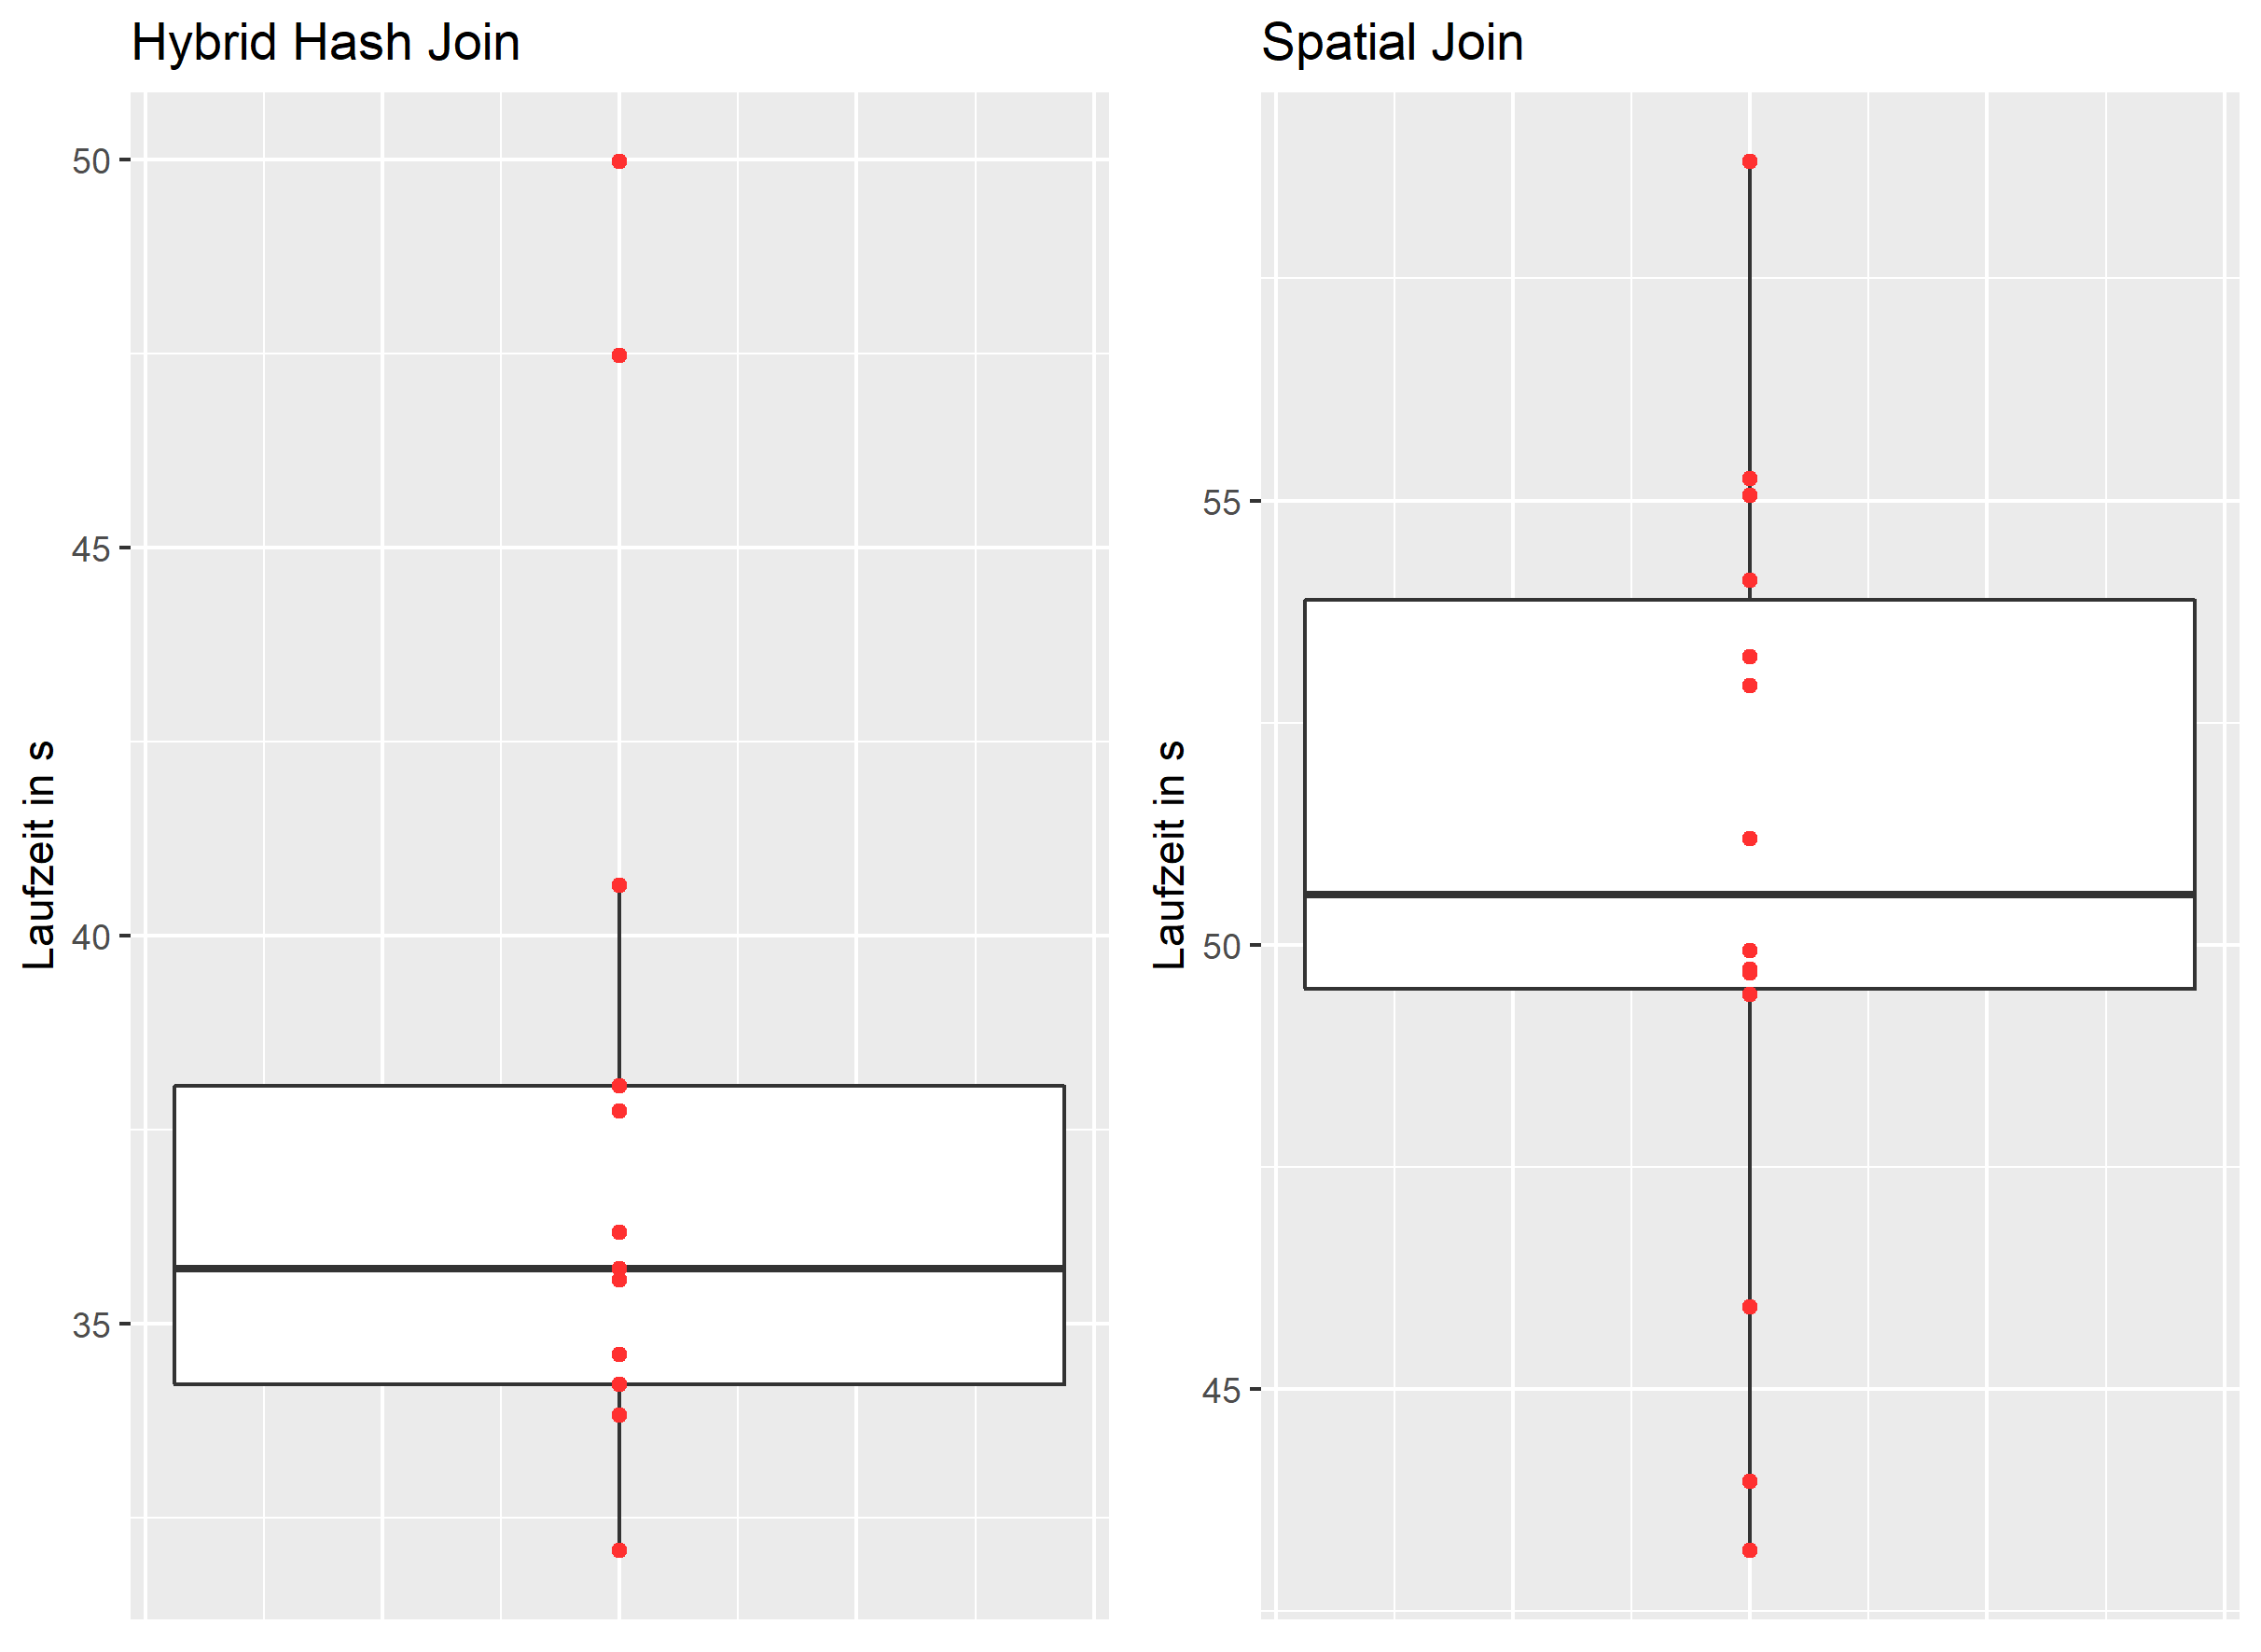
\includegraphics[width=0.70\textwidth]{Bilder/streuung.png}
	\caption{Mehrfache Ausführung der gleichen Hash-Joins $roads \bowtie roads$ und Spatial-Joins $roads \bowtie waterways$.}
	\label{img:streuung}
\end{figure}

Sofern Laufzeiten für die Effizienztest und Experimente gemessen werden, wird die Ausgabe der vergangenen Zeitdauer (\Fb{elapsed time}) und die CPU-Zeit nach Ausführung einer Anfrage in \Fb{SecondoTTYBDB} verwendet. Die vergangene Zeitdauer ist die Differenz der Zeitstempel beim Start der Anfrage und bei Abschluss. Die CPU-Zeit ist die Zeit, die vom Prozessor verbraucht wird, also die reine Berechnungszeit ohne die Zeit, die der Prozessor beispielsweise auf I/O-Operationen oder andere Prozesse wartet (zum Beispiel Join-Aufrufe oder das Warten auf Nachrichten). Da jeder Thread Prozessor-Zeit verbraucht, ist für diese Arbeit hier vor allem die vergangene Zeitdauer interessant, aber die CPU-Zeit kann Hinweise darauf geben, wie gut eine Parallelisierung gelungen ist, da im optimalen Fall und wenn in der Anfrage nur ein paralleler Operator verwendet wurde, die CPU-Zeit die genutzte Threadzahl multipliziert mit der verbrauchten Zeitdauer ergeben muss. Dies würde bedeuten, dass während der gesamten Laufzeit alle Kerne dauerhaft genutzt worden sind. Im Gegensatz zu den Single-Thread-Varianten der Operatoren ist die Laufzeit der Multi-Thread-Operatoren nicht stabil, da die Verteilung auf die Threads in den meisten Fällen nicht immer gleich ist und die Synchronisationsmechanismen sind nicht vorhersagbar. \autoref{img:streuung} zeigt die Verteilung von Laufzeiten bei mehrmaliger Ausführung eines Spatial-Joins und eines Hash-Joins. Dieses Verhalten der Operatoren macht die Interpretation der Messergebnisse schwierig, insbesondere wenn keine deutliche Tendenz zu erkennen ist. Allerdings wurden alle Tests mehrfach ausgeführt und per Augenschein überprüft, ob Ergebnisse stark variieren. Zumindest Extremwerte wurden so versucht auszuschließen.  

Für die Testes der Operatoren verwende ich den Berlin-Datensatz von Open Streetmap, der mit dem Stand 7.1.2020 heruntergeladen worden ist (siehe \autoref{tab:testRel})\footnote{\url{http://download.geofabrik.de/europe/germany/berlin.html}}.

\begin{table}
	\centering
\begin{tabular}{|c|c|c|c|}
	\hline 
	Tabelle & Anzahl Tupel & Quelle & räumlicher Datentyp  \\ 
	\hline 
	buildings & 502.309 & gis\_osm\_buildings\_a\_free\_1 & region \\ 
	\hline 
	landuse & 29.341 & gis\_osm\_landuse\_a\_free\_1 & region \\ 
	\hline 
	natural & 116 & gis\_osm\_natural\_a\_free\_1 & region \\ 
	\hline 
	natural2 & 162.112 & gis\_osm\_natural\_free\_1 & point \\ 
	\hline
	places & 108 & gis\_osm\_places\_free\_1 & region \\ 
	\hline 
	pois & 66.123 & gis\_osm\_pois\_free\_1  & point \\ 
	\hline 
	roads & 181.685 & gis\_osm\_roads\_free\_1 & line \\ 
	\hline
	traf & 40.650 & gis\_osm\_traffic\_free\_1  & point \\ 
	\hline 
	waterways & 2104 & gis\_osm\_waterways\_free\_1 & line \\ 
	\hline
	strassen & 3212 &  berlintest & line \\ 
	\hline
	WFlaechen & 85 &  berlintest & region \\ 
	\hline 
	WStrassen & 21 &  berlintest & line \\ 
	\hline 
	Plaetze & 201 &  berlintest & point \\ 
	\hline 
	Orte & 506 & berlintest & keine \\ 
	\hline
	plz & 41267 & berlintest & keine \\ 
	\hline 
\end{tabular}
\caption{\label{tab:testRel} Übersicht über in Tests und Experimenten verwendeten Relationen}
\end{table}

Da es mehrfach Probleme mit \Fb{FLOBs} gab, nutze ich auch Versionen der Relationen, in denen Attribute des Typs \Fb{FText} in \Fb{string} umgewandelt worden sind. Kennzeichen für diese Relationen ist das Postfix \Fb{\_str}.

\subsubsection{Funktionstest MThreadedsort}

Auf Korrektheit wird mit zwei Methoden getestet. Es ist notwendig, dass ein Test mit \Fb{--valgrindlc} ohne Fehler abläuft und das Ergebnis muss den Erwartungen entsprechen, das heißt, eine Relation muss entsprechend der Parameter korrekt sortiert werden. Eine Korrektheit kann nur festgestellt werden, wenn garantiert ist, dass der Code des Operators in der Summe der Tests vollständig durchlaufen worden ist, was mit Ausgaben abgesichert wird, die in der endgültigen Version des Operators entfernt worden sind. Um dies zu garantieren, muss die Relation so groß sein, dass Läufe persistiert werden müssen bzw. wenig Hauptspeicher zur Verfügung stehen und es sollen mehr als zwei Läufe in der suboptimalen Phase verschmolzen werden müssen. In der postoptimalen Phase sollen die Feeder mit ein und zwei Eingängen getestet werden und es soll ein Mergepipeline-Baum konstruiert wird, der nicht lediglich Blätter und eine Wurzel enthält. Dementsprechend wird mit 3, 4 und 6 Threads getestet \footnote{Der Hauptthread, in dem der Secondo-Kern und damit auch das Scheduling läuft, zählt immer mit}. Darüber hinaus wird mit einer Threadzahl getestet, die deutlich über der Kernzahl des System liegt (16), da in diesem Fall Threads zwischenzeitlich pausieren müssen. Auch wenn dies nicht für die Performance nicht ungedingt sinnvoll ist, hat dies Auswirkungen besipielsweise auf die Buffer und auch in diesem Fall muss der Operator korrekt funktionieren, da unter Anwendungs-Bedingungen nicht unbedingt bekannt ist, wie viele Kerne genutzt werden können oder eventuell durch andere Programme verwendet werden.

\begin{minipage}{\linewidth}
	\begin{lstlisting}[caption={Beispiel Testqueries für den Sort-Operator}, label=list:testsort]
	query buildings feed mThreadedMergeSort[Name] count
	query buildings feed mThreadedMergeSort[Name] {memory 12} project[Name] count
	\end{lstlisting}
\end{minipage}

Mit \Fb{--valgrindlc} terminiert der Operator nur in einem Fall mit einem Speicherloch, nämlich sofern der Operator nicht vollständig speicherintern ablaufen kann. Ein Zeiger auf eine CcInt wird nicht gelöscht. Dies ist allerdings nicht ein Fehler meines Operators, sondern ein bekannter Fehler des Queryprozessors, der auftritt, wenn der Queryprozessor Konstanten verwendet. Sofern mehr Threads verwendet werden als Kerne zur Verfügung stehen, kann es zu einem Deadlock kommen, 

\begin{minipage}{\linewidth}
	\begin{lstlisting}[caption={Beispiel Testqueries für den Sort-Operator}, label=list:testsort]
	query (roads_str feed mThreadedMergeSort[NameStr] project[NameStr]) = (roads_str feed sortby[NameStr] project[NameStr]) 
	\end{lstlisting}
\end{minipage}

Korrektheit wird mit unterschiedlich großen Relationen und der Memory-Option, um sicherzustellen, dass alle Persistierungsstrukturen durchlaufen werden, mit unterschiedlichen vielen Threads getestet. Im Unterschied zu den anderen Operatoren läuft nicht in jedem Thread der gleiche Algorithmus ab, sondern der Aufbau der Merge-Pipeline unterscheidet sich bezüglich der Anzahl genutzter Threads. Unterschiede bestehen zwischen einer geraden und ungeraden Threadzahl und der Notwendigkeit von Zwischenschritten, die erst ab 5 Threads (plus einen Hauptthread) verwendet werden müssen. Wichtig ist es hier, die Ergebnisrelation auf die Sortierattribute zu projezieren, da meine Implementierung eines Multithread-Sort nicht die Reihenfolge der Relation aufrecht erhält, das heiß, die Ergebnisrelation kann sich bei Duplikaten in den Sortierattributen in der Reihenfolge nicht für die Sortierung genutzten Attributen unterscheiden. Es wird lediglich garantiert, dass richtig sortiert wird, aber die Reihenfolge in den Nicht-Sortierattributen kann bei jeder Abfrage auch bei genau identischen Parametern unterschiedlich sein. Zusätzlich werden die Ergebnisse überprüft, wenn mehr als ein Sortierattribut verwendet wird und für eine invertierte Sortierreihenfolge.

\begin{table}
	\centering
\begin{tabular}{|c|c|c|c|}
	\hline 
	Threads\footnotemark & speicherintern & project & Ergebnis \\ 
	\hline 
	3 & ja & ja & true \\ 
	\hline 
	3 & nein & ja & true \\ 
	\hline 
	4 & ja & ja & true \\ 
	\hline 
	4 & nein & ja  & true \\ 
	\hline 
	6 & ja & ja & true \\ 
	\hline
	6 & nein & ja & true \\ 
	\hline
	6 & ja & nein & false \\ 
	\hline 
\end{tabular}
\caption{\label{tab:testSort} Threadzahl und zur Verfügung stehender Hauptspeicher beim MergeSort}
\end{table}

\footnotetext{inkl. Hauptthread und Scheduling. Für das Sortieren und die Merge-Pipeline steht also ein Thread weniger zur Verfügung}

\begin{table}
	\centering
	\begin{tabular}{|c|c|}
		\hline 
		Sortierattribute & Ergebnis \\ 
		\hline 
		 Oneway, Maxspeed, Fclass, NameStr &  true \\ 
		\hline 
		NameStr, FALSE &  true \\ 
		\hline 
	\end{tabular}
	\caption{\label{tab:testSortAttr} Sortierattribute und Reihenfolge beim MergeSort}
\end{table}


Der Operator funktioniert nicht, sofern \Fb{FLOBs} Sortierattribute sind. Ein konkurrierender Zugriff auf sie führt zu einem falschen Ergebnis -- für den Vergleich werden die vollständigen Objekte fehlerhaft in den Speicher gelesen. Wenn aber eine Relation lediglich \Fb{FLOBs} als Attribute hat, diese aber keine Sortierkriterien sind gibt es keine Probleme. Deswegen werden Sortierattribute von Typen, die als \Fb{FLOBs} angelegt sind, ausgeschlossen. TODO

Im folgenden werde ich den Operator auf Robustheit testen. Die Ergebnisse sind in \autoref{tab:testSortRobust} zusammengestellt. Als Beispiele für eine spezielle Verteilung der Eingangsrelation wird eine vollständig sortierte Eingangsrelation getestet. In diesem Fall müssen auch bei sehr großen Relationen keine Daten temporär gespeichert werden. Vergleichbares gilt, wenn nach Attributen sortiert wird, die nur sehr wenige Ausprägungen haben, wobei hier nicht garantiert ist, dass keine Daten zwischengespeichert werden müssen. Leere Eingangsströme bzw. Relationen als Eingang, die nur sehr wenige Tupel beinhalten, können dazu führen, dass alle oder einzelne Sortierthreads keine Daten zugewiesen bekommen. Die weiteren Tests betreffen eine Parametrisierung, die nicht sinnvoll oder fehlerhaft ist und vom Type-Mapping abgefangen bzw. behandelt wird. Dieser wie auch alle anderen Operatoren funktionieren nur, wenn sie mindestens 3 Kerne verwenden; 2 für die Worker und 1 für den Hauptthread und das Scheduling. Dieser Operator funktioniert nicht richtig und ist auch nicht sinnvoll, wenn mehr Kerne verwendet werden, als das System zur Verfügung hat. Dann kann es zu Deadlocks in der Merge-Pipeline kommen. Da für diesen Operator kein Performancevorteil zu erwarten ist, wird die Threadzahl in diesem Fall auf die maximale Kernzahl des Systems gesetzt. Sofern keine Sortierreihenfolge angegeben ist, wird automatisch aufwärts sortiert (TRUE). Eine Besonderheit in dem Type-Mapping dieses Operators ist es, dass Sortierattribute, die nicht Teil der Relation sind, lediglich ignoriert werden. Das Type-Mapping gibt allerdings einen Fehler aus, wenn gar kein gültiges Sortierattribut angegeben wird. Das letzte Testbeispiel zeigt, wie eine Sortierliste mit Fehlern gewandelt wird.

\begin{table}
	\centering
	\begin{tabular}{|p{7.5cm}|p{7.5cm}|}
		\hline 
		Test & Ergebnis \\
		\hline
		Eingang vollständig vorsortiert & TRUE, keine Anlage temporärer Dateien \\
		\hline
		Sortierattribut Maxspeed,\newline wenig Ausprägungen & TRUE  \\
		\hline
		mit 2 Kernen & only works with $\geq$ 3 threads  \\ 
		\hline
		mit 20 Kernen & uses max system cores only: 6 \\ 
		\hline
		Eingangsstrom leer & leere Ergebnisrelation \\ 
		\hline
		Eingangsstrom 2 Tupel & Ergebnisstrom 2 Tupel \\ 
		\hline
		Eingang kein Strom & first arg is not a tuple stream \\ 
		\hline
		automatische Setzung Sortierreihenfolge & nicht angegebenes TRUE wird ergänzt \\ 
		\hline
		Sortierattribut nicht Teil der Relation & did not find any attribute \\ 
		\hline
		Sortierreihenfolge nicht boolean & automatische Setzung TRUE \\ 
		\hline
		kein Sortierattribut & list corrupt \\
		\hline
		Oneway, NoAttr, FALSE, Maxspeed,\newline Fclass, FALSE, NameStr &  Oneway TRUE Maxspeed TRUE\newline Fclass FALSE NameStr TRUE \\
		\hline
\end{tabular}
	\caption{\label{tab:testSortRobust}Robustheit Merge-Sort}
\end{table}

Effizienz wird hier verglichen mit dem Operator Fb{sortb} für die Relation \Fb{roads\_str} einerseits mit eine Sortierung nach dem Straßennamen (siehe \autoref{img:sortKern}) und andererseits nach mehreren Sortierattributen (\Fb{Fclass, Oneway, Bridge, Tunnel, Code, NameStr}) (siehe \autoref{img:sortKernMf}). Bei der Nutzung von 3 Kernen ist die von mir implementierte Variante schneller als die Single-Thread-Version, sofern nach mehreren Attributen sortiert wurde, und ungefähr gleich schnell, wenn nur nach einem Attribut sortiert wurde. Für die Sortierung nach mehreren Attributen wurden diese so gewählt, dass für die Bestimmung der Reihenfolge meist ein Vergleich aller Attribute notwendig ist, da die zuerst zu berücksichtigen Attribute sehr wenige Ausprägungen haben.  

Bemerkenswert ist es, dass sich das Laufzeitverhalten mit der Anzahl genutzter Kerne verschlechtert und zwar sprunghaft ab drei bzw. vier Kernen, wobei anschließend eine leichte Verbesserung eintritt. Einige Faktoren tragen zu diesem Verhalten bei: Nur bei $4, 8, 16, \ldots$ Worker-Threads \footnote{Ein Kern wird bei allen Operatoren für das Scheduling verwendet} ist die Merge-Pipeline-Baum ausgeglichen -- in den anderen Fällen kann es dementsprechend zu Wartezeiten in den entsprechenden Knoten der Pipeline kommen. Eine Vorsortierung wird bei der Nutzung von vielen Threads nicht gut genutzt, da sortierte Folgen auf unterschiedliche Worker verteilt werden. Abschließend vermute ich, dass der Flaschenhals vor allem in der Synchronisation der Warteschlangen liegt, die als Datenaustauschstruktur zwischen den einzelnen Elementen der Merge-Pipeline dient, da das Laufzeitverhalten vor allem an den Punkten schlechter wird, an denen eine Ebene in der Merge-Struktur zugefügt wird. 

Eine weitere Kennzahl unterstützt diese Interpretation: Der Koeffizient aus vergangener Zeit und CPU-Zeit, der als Maß für die Parallelisierung genommen werden kann (sofern andere Einflüsse wie I/O-Operationen gleich bleiben) sinkt von 3 (0.69) zu 10 Kernen (0.397918) deutlich, aber nicht linear, sondern mit der Anzahl genutzter Kerne langsamer. Da auch die genutzte CPU-Zeit steigt, ist davon auszugehen, dass bei der Nutzung von mehr Kernen deutlich größere Verluste durch das Overhead für die Parallelisierung eintreten. 

\begin{figure}
	\centering
	\subfloat[\Fb{roads\_str} nach dem Straßennamen\label{img:sortKern}]{{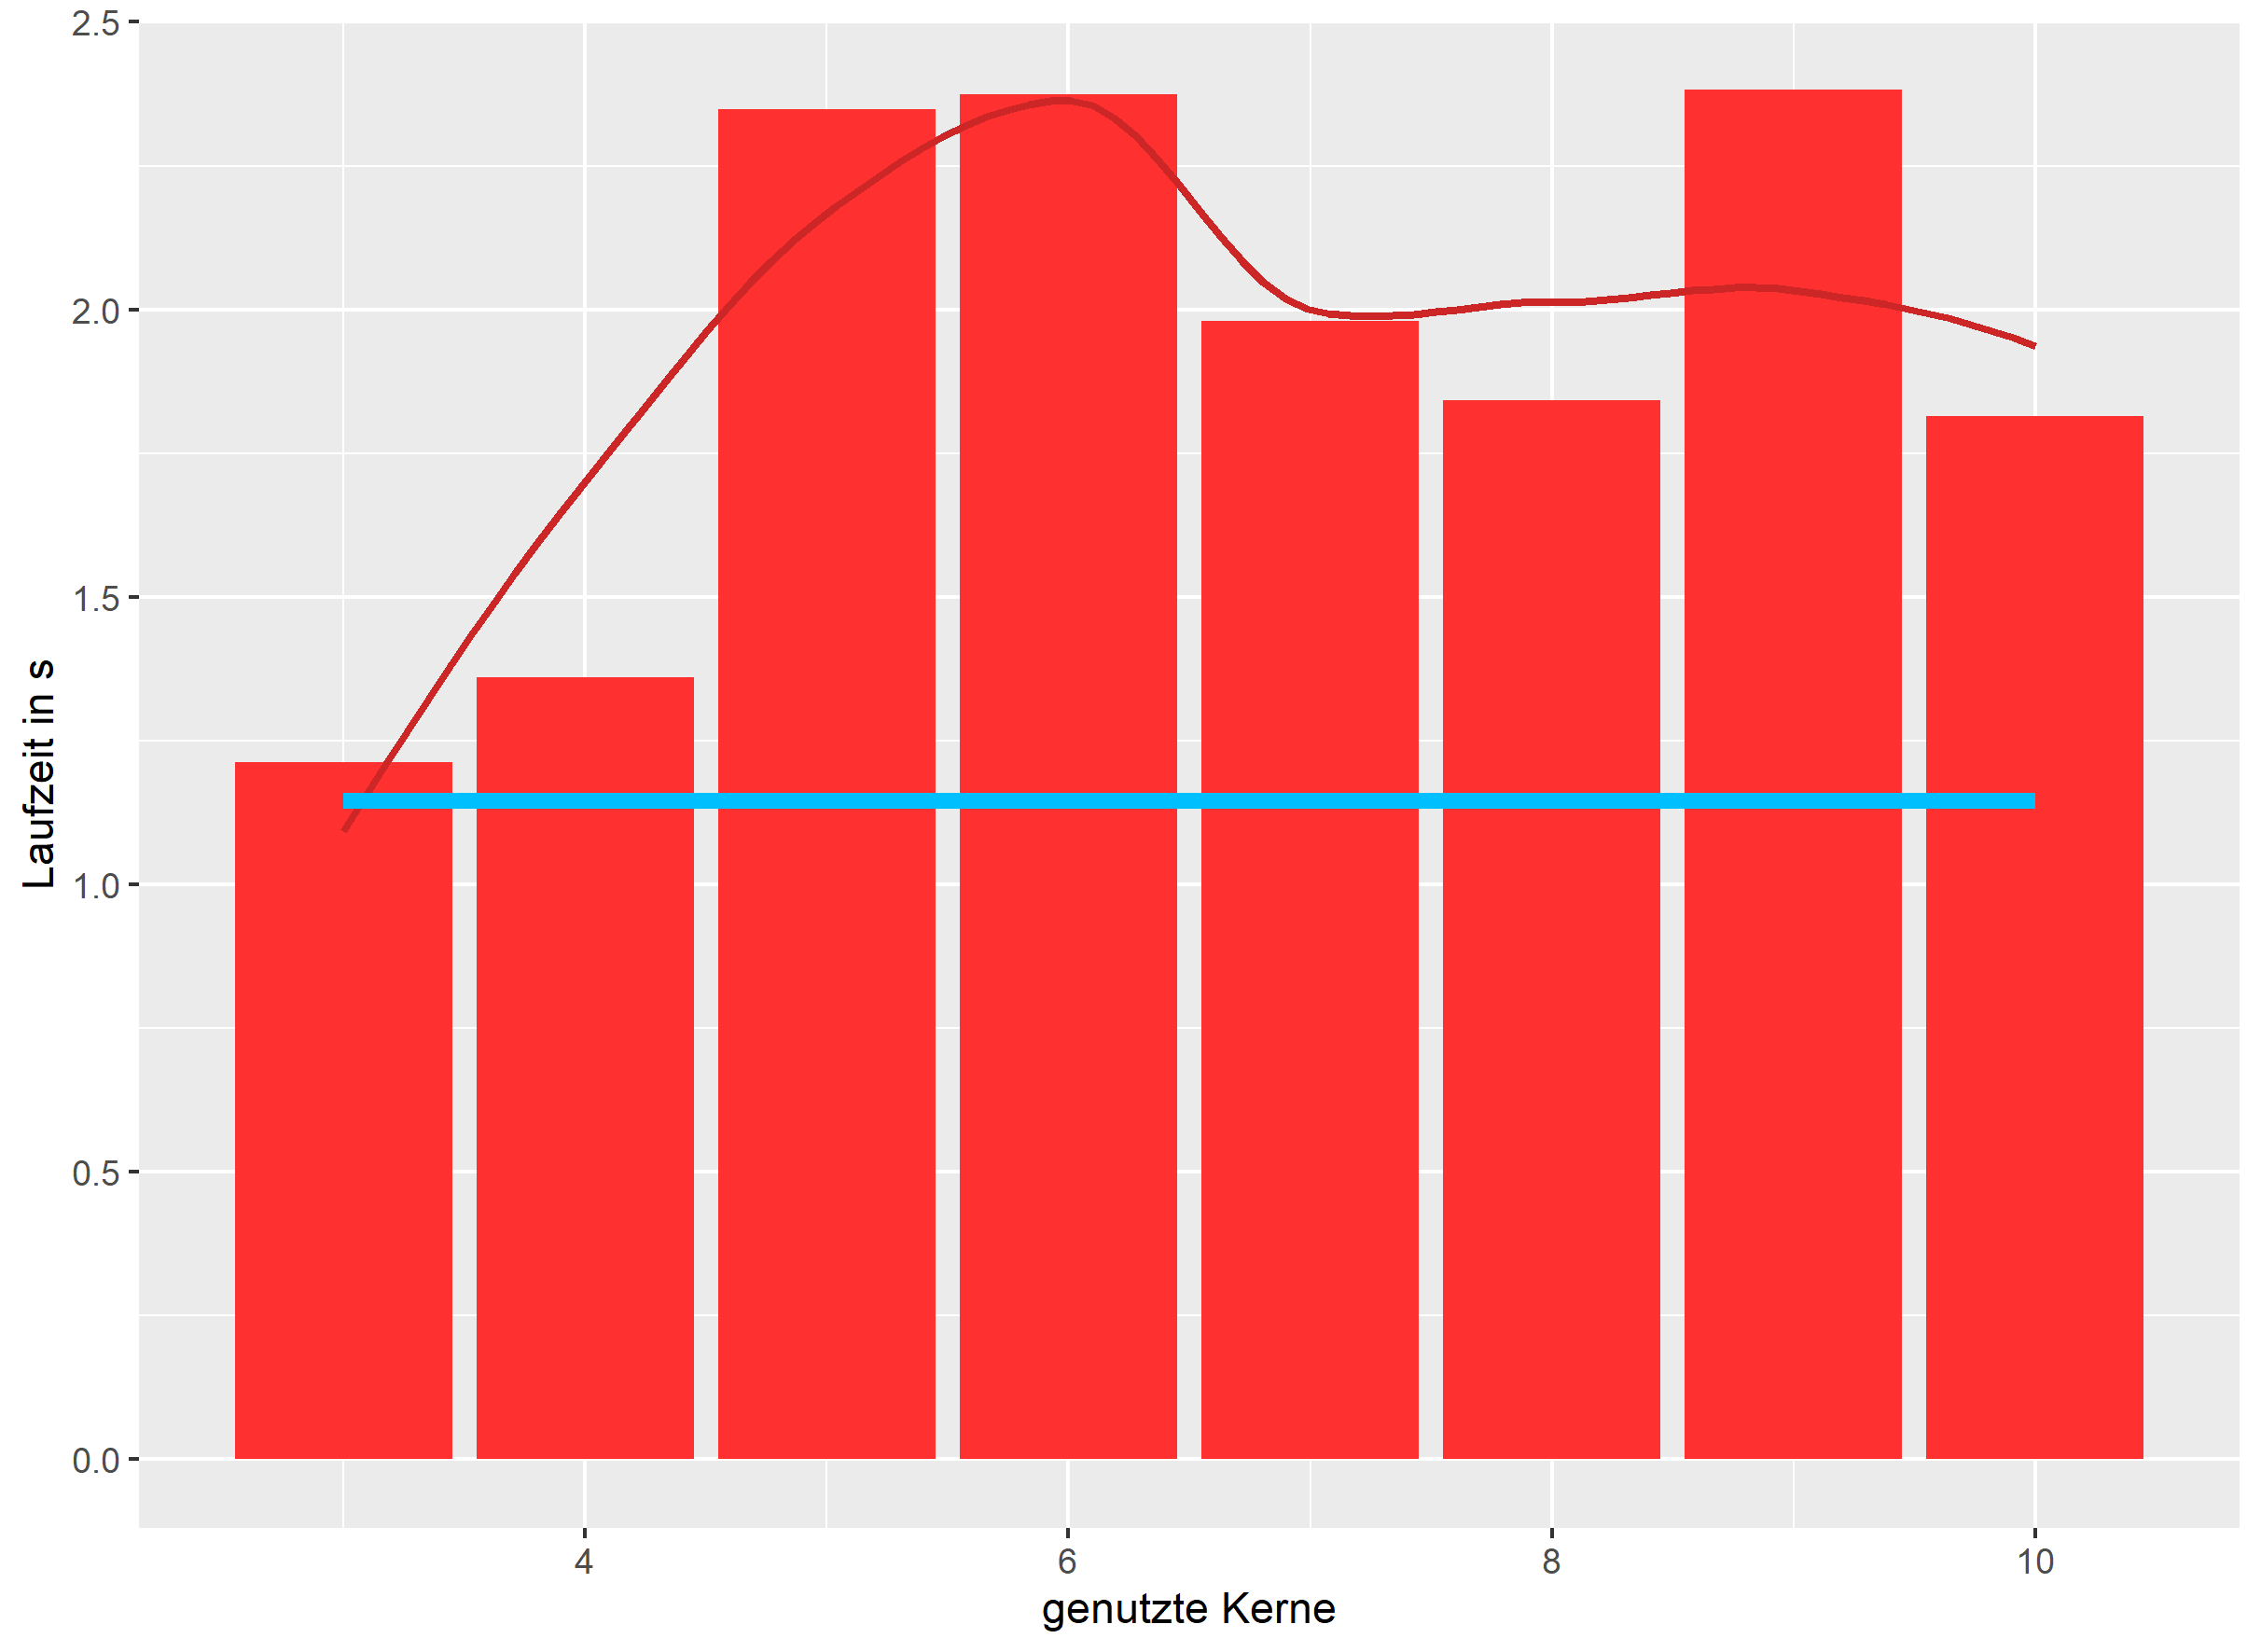
\includegraphics[width=0.45\linewidth]{Bilder/sort_kerne.png}}}
 	\qquad
 	\subfloat[\Fb{roads\_str} nach vielen Attributen\label{img:sortKernMf}]{{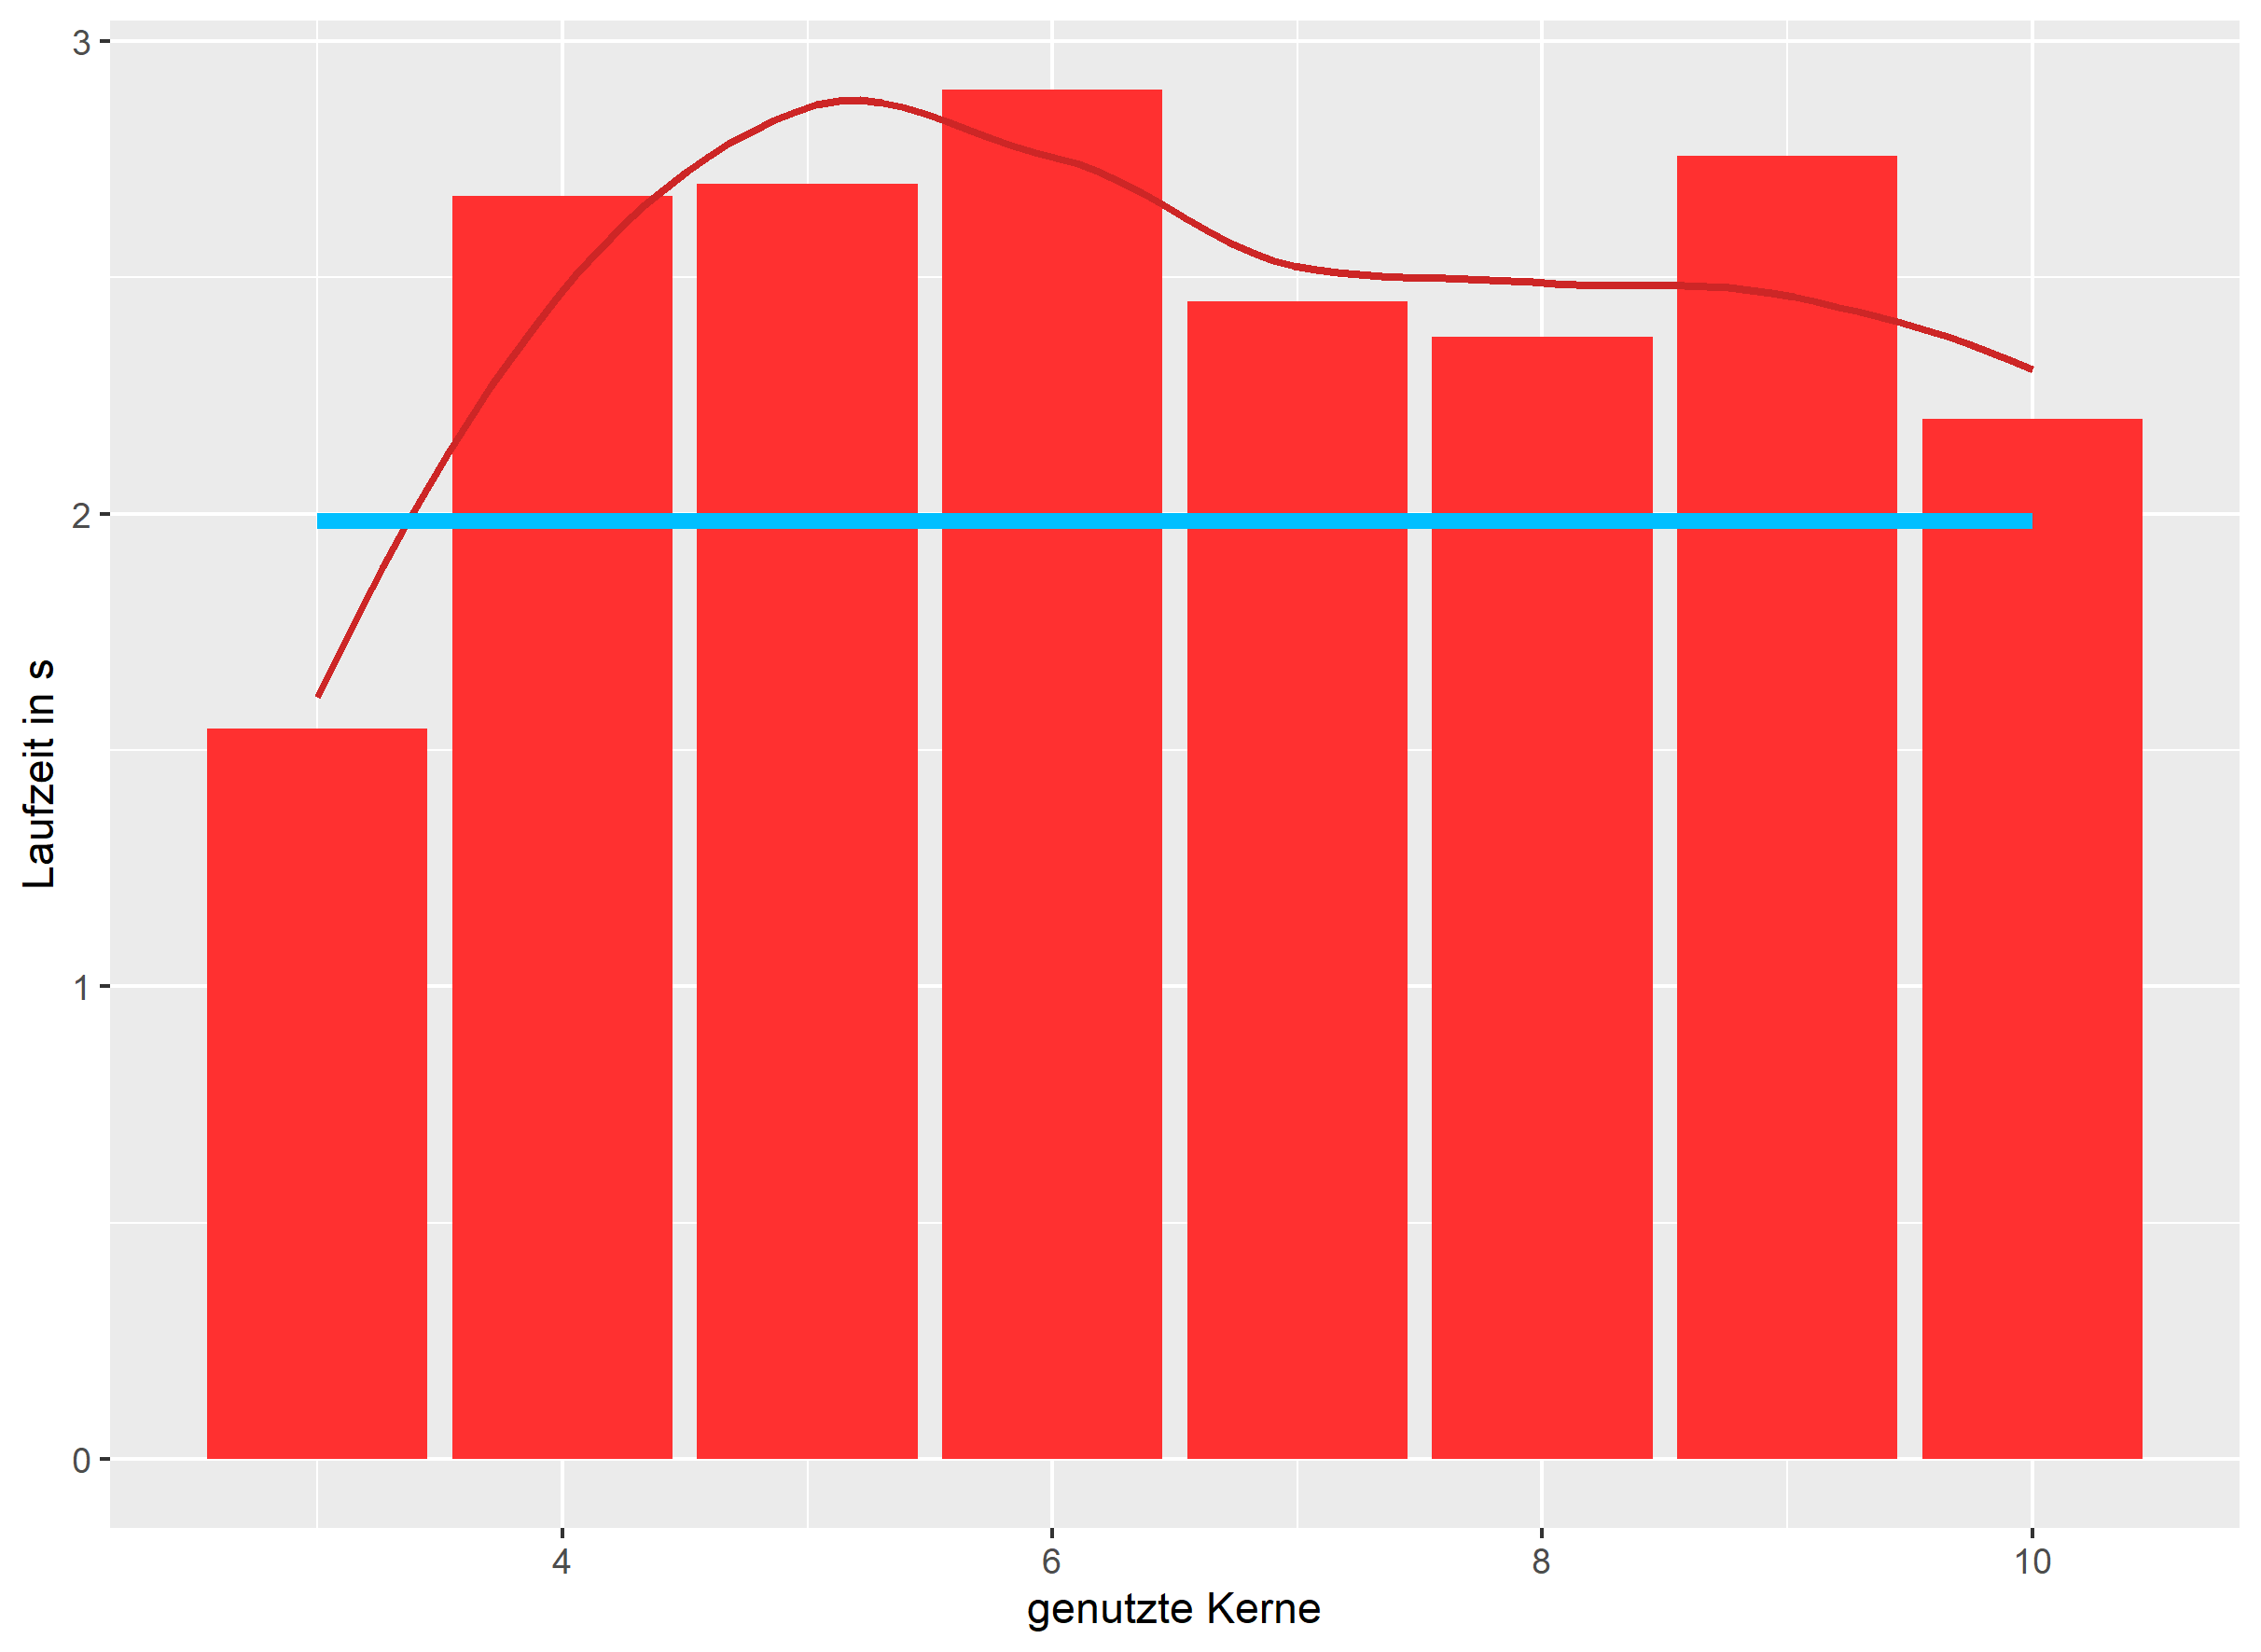
\includegraphics[width=0.45\linewidth]{Bilder/sort_kerne_mf.png}}}
	\caption{Sortierung und Anzahl Kerne. Blaue Gerade: Single-Thread-Operator im Vergleich, rote Linie: Glättungskurve.}
	\label{img:sortKernAlg}
\end{figure}

\subsubsection{Funktionstest MThreadedHashJoin}

Der Multithreading-Hashjojn-Operator verfügt über eine komplexe Überlaufstrukturen. Zu einem Überlauf kommt es vor allem bei sehr großen Relationen und vor allem einer unausgeglichenen Verteilung über Join-Attribute in der R-Relation. Dementsprechend ist es hier für einen Test auf Korrektheit insbesondere wichtig sicherzustellen, dass in der Gesamtheit der Tests alle Teilbereiche des Codes durchlaufen werden. Um das zu kontrollieren, habe ich für die Testphase in den verschiedenen Methoden bzw. Abzweigen für Overflow-Handling Ausgaben an die Konsole eingebaut. Getestet wurde eine Join der \Fb{roads\_str}-Relation mit sich selbst. Da die Relationen im Attribut \Fb{Name} einen großen Anteil von Leerstrings hat, haben dementsprechend sehr viele Tupel einen gleichen Hashwert und der Join nähert sich einem kartesische Produkt. Selbstverständlich ist für solch einen Join ein Hash Join keine sinnvolle Wahl, aber die Verteilung innerhalb der Relation stellt sicher, dass die Overflow-Behandlung vollständig durchlaufen wird. Eine Schwierigkeit war es, dass die Join-Operatoren der \Fb{ExtRelationC++}-Algebra nicht stabil sind -- bei großen Relationen mit speicherintensiven Tupeln und sehr großen Ergebnisströmen kam es häufig zu abstürzen. \autoref{tab:testJoin} zeigt die Ergebnisse dieser Tests -- zusätzlich zu dem durchgeführtem Join wird die genutzte Kernzahl, die Speichereinschränkung und die Verkürzung der Relation mit dem \Fb{head}-Operator angegeben. Um einen Fehler auszuschließen, der bei den Single-Thread-Join-Operatoren auftritt, habe ich einen Hybrid-Hash-Join mit 2 großen Relationen, mit denen die Single-Thread Varianten nicht mehr funktioniert haben, ausgeführt, aber nur die Ausführung ohne Absturz dokumentiert. Allerdings tritt, wenn nicht wie hier zwei Relationen verglichen werden, sondern eine neue Relation erzeugt wird, auch ein Fehler auf, der mehrfach bei den Single-Thread-Varianten des Join-Operators aufgetreten ist: Der Operator bricht mit einer Fehlermeldung des Storage-Managers ab, nämlich \Fb{DbEnv: BDB2055 Lock table is out of available lock entries}. Da dieser Fehler aber nicht nur bei meinem Operator, sondern bei den anderen Join-Operatoren noch in viel größerem Maße auftritt, gehe ich von einem Fehler im Secondo-Kern aus.

\begin{minipage}{\linewidth}
	\begin{lstlisting}[caption={Beispiel Testqueries für den Join-Operator}, label=list:testjoinsort]
	query (roads_str feed head[5000] {p} roads_str feed {o} mThreadedHybridJoin[NameStr_p, NameStr_o] project[NameStr_o] sortby[NameStr_o]) = (roads_str feed head[5000] {p} roads_str feed {o} sortmergejoin[NameStr_p, NameStr_o] project[NameStr_o] sortby[NameStr_o])
	\end{lstlisting}
\end{minipage}

Zusätzlich habe ich noch Tests mit kleinen und gleichmäßiger verteilten Relationen der Datenbank \Fb{berlintest} durchgeführt, um das Verhalten des Operators bei unterschiedlicher Nutzung an Kernen und Speicher zu untersuchen. 

\begin{table}
	\centering
	\begin{tabular}{|c|c|c|c|c|}
		\hline 
		Operation & head/memory & Kerne & Overflow-Strukturen & Ergebnis \\ 
		\hline 
		$roads\_str \bowtie roads\_strf$ & 10.000/all & 5 & keine & true \\ 
		\hline 
		$roads\_str \bowtie roads\_str$ & 10.000/2~MB & 5 & keine & true \\ 
		\hline 
		$roads\_str \bowtie roads\_str$ & 20.000/all & 5 & keine & 50.764.348 \\ 
		\hline 
		$pr\_sj\_pr\footnotemark \bowtie pois\_str$ & 30.000/2~MB & 5 & 2 rekursiver Overflow & true \\ 
		\hline 
		$strassen \bowtie Plaetze$ & all/2~MB & 6 & keine  & true \\ 
		\hline
		$strassen \bowtie Plaetze$ & all/all & 3 & keine & true \\ 
		\hline
		$strassen \bowtie Plaetze$ & all/all & 6 & keine & true \\ 
		\hline
		$Orte \bowtie plz$ & all/2~MB & 6 & keine & true \\ 
		\hline
	\end{tabular}
	\caption{\label{tab:testJoin} Korrektheitsnachweis durch Vergleich Single- und Multi-Thread-Version.}
\end{table}

\footnotetext{Die Relation pr\_sj\_pr ist ein Spatial Join zwischen pois und roads.}

Für eine Vielzahl unterschiedlicher Relationen und deren Kombinationen wurde bereits getestet. Auch funktioniert der Operator weitestgehend gut mit sehr großen Relationen. Hier ist aber anzumerken, dass, wenn die Gesamtheit der Tupel der R-Relation, deren Joinattribut den gleichen Hashwert hat, nicht in den Hauptspeicher passen, diese nicht vollständig behandelt werden, da sonst eine zusätzliche Persistierungsstruktur für einzelne Buckets implementiert werden müsste. In der jetzigen Implementierung werden hier nur die Tupel ignoriert, die nicht mehr in den Hauptspeicher passen. Sinnvoller wäre sicher, den Operator mit einer Fehlermeldung abbrechen zu lassen.

Problematisch kann es auch sein, wenn die Eingangsströme entweder ganz leer sind oder so wenige Tupel enthalten, dass eine Partitionierung auf alle Threads nicht möglich ist. Darüber hinaus wird getestet, ob im Type-Mapping Parameter zurückgewiesen werden, die für einen Equi-Join nicht sinnvoll sind. Die vorgenommenen Robustheitstest werden in \autoref{tab:testJoinRobust} dargestellt, wobei die Tests immer bei der Verwendung von 6 Kernen und mit den beiden Relationen \Fb{strassen} sowie \Fb{Plaetze} ausgeführt worden sind, außer wenn es anders vermerkt wurde. Alle durchgeführten Test entsprachen den Erwartungen.

\begin{table}
	\centering
	\begin{tabular}{|p{7.5cm}|p{7.5cm}|}
		\hline 
		Test & Ergebnis \\
		\hline
		Eingangsstrom leer & leere Ergebnisrelation \\ 
		\hline
		Eingangsstrom 2 Tupel & 2 TODO manchmal Deadlock \\ 
		\hline
		Join-Attribute ohne Übereinstimmungen & TRUE, keine Anlage temporärer Dateien \\
		\hline
		mit 2 Kerne & TRUE  \\
		\hline
		mit 20 Kernen & only works with $\geq$ 3 threads  \\ 
		\hline
		Attribute nicht gleicher Typ & TODOm \\ 
		\hline
		erstes Attribute nicht Teil der Relation & Name\_o is not an attribute of the second stream \\ 
		\hline
		Eingang R kein Strom & first arg is not a tuple stream \\ 
		\hline
		Eingang S kein Strom & second arg is not a tuple stream \\ 
		\hline
		kein Join-Attribut & stream(tuple) x stream(tuple) x attr1 x attr2 expected \\ 
		\hline
		3 Join-Attribute & stream(tuple) x stream(tuple) x attr1 x attr2 expected \\
		\hline
		3 Eingangsströme &  Syntax error \\
		\hline
	\end{tabular}
	\caption{\label{tab:testJoinRobust}Robustheit Merge-Sort}
\end{table}

Die Effizienz des Operators wird hier nur für Joins von Relationen untersucht, deren Verteilung den Einsatz eines Hash-Joins sinnvoll erscheinen lässt. Dies bedeutet vor allem, dass in den Relationen wenig Duplikate in den Join-Attributen vorkommen, die einerseits zu einer sehr großen Anzahl von Ergebnistupeln führen und andererseits alle den gleichen Hashwert haben. Dies würde zu Performanceproblemen für einen Hashjoin führen, der nur eine gute Effizienz hat, wenn die Tupel gleichmäßig auf die Buckets verteilt werden. Genauer wird das Verhalten bei unterschiedlichen Verteilungen in \autoref{exp:hash} betrachten. Vergleichen wird der \Fb{mThreadedHybridJoin} mit seiner Single-Thread-Variante, dem \Fb{hybridhashjoin} mit 100 und 1000 Buckets unter Nutzung einer verschiedenen Anzahl von Kernen. \autoref{img:joinKern} zeigt die Laufzeitanalyse eines Selfjoins der Relation \Fb{roads\_str} -- die verwendete Relation hat 44.684 Tupel und wegen einer Duplikate in den Straßennamen ergibt der Join 841.036 Tupel als Ergebnis. \autoref{img:joinKernBe} zeigt zwei Relatione der Datenbank \Fb{berlintest}. Bei $Strassen \bowtie Plaetze$ ist die R-Relation wesentlich größer als die S-Relation und liefert nur 15 Tupel als Ergebnis, bei $Orte \bowtie PLZ$ ist die R-Relation deutlich kleiner und der Join liefert 10.052 Tupel als Ergebnis.

Die Multithrad-Variante ist in allen Fällen nicht so effizient wie die Singlethread-Variante. Allerdings können aus dem Verhalten bei einer unterschiedlichen Zahl genutzter Kerne der verschiedenen Joins Rückschlüsse darauf gezogen werden, wo genau die Performanceprobleme des Operators liegen. Im Detail werde ich dies unter Berücksichtigung weiterer Experimente in \autoref{exp:hash} diskutieren. Am besten im Vergleich zur Singlethread-Variante schneidet der Operator ab, wenn die R-Relation sehr klein ist. Die Größe der S-Relation dagegen scheint wenig Einfluss zu haben, da sie beim Selfjoin und bei $Orte \bowtie PLZ$ ungefähr gleichgroß ist. Also liegt vor allem ein Problem beim Aufbau der Hash-Tabellen vor. Einerseits benötigt meine Implementierung einen Scan über die R-Relation mehr als die Singlethread-Variante für die Partitionierung. Andererseits wird in jedem Thread nur das erste Bucket direkt auf eine Hashtabelle verteilt, die anderen entweder im Speicher oder in einem Tupelfile zwischengespeichert. Dieser Ansatz wurde so gewählt, da er einfacher zu implementieren ist, weil Persistierungsstrukturen genauso behandelt werden können wie speicherinterne Strukturen. Aber hier wäre es sicher sinnvoll, einen Ansatz zu wählen, der, sofern genug Hauptspeicher zur Verfügung steht, direkt Hashtabellen berechnet auch für die Buckets, die nicht im ersten Ablauf behandelt werden. 

\begin{figure}
	\centering
	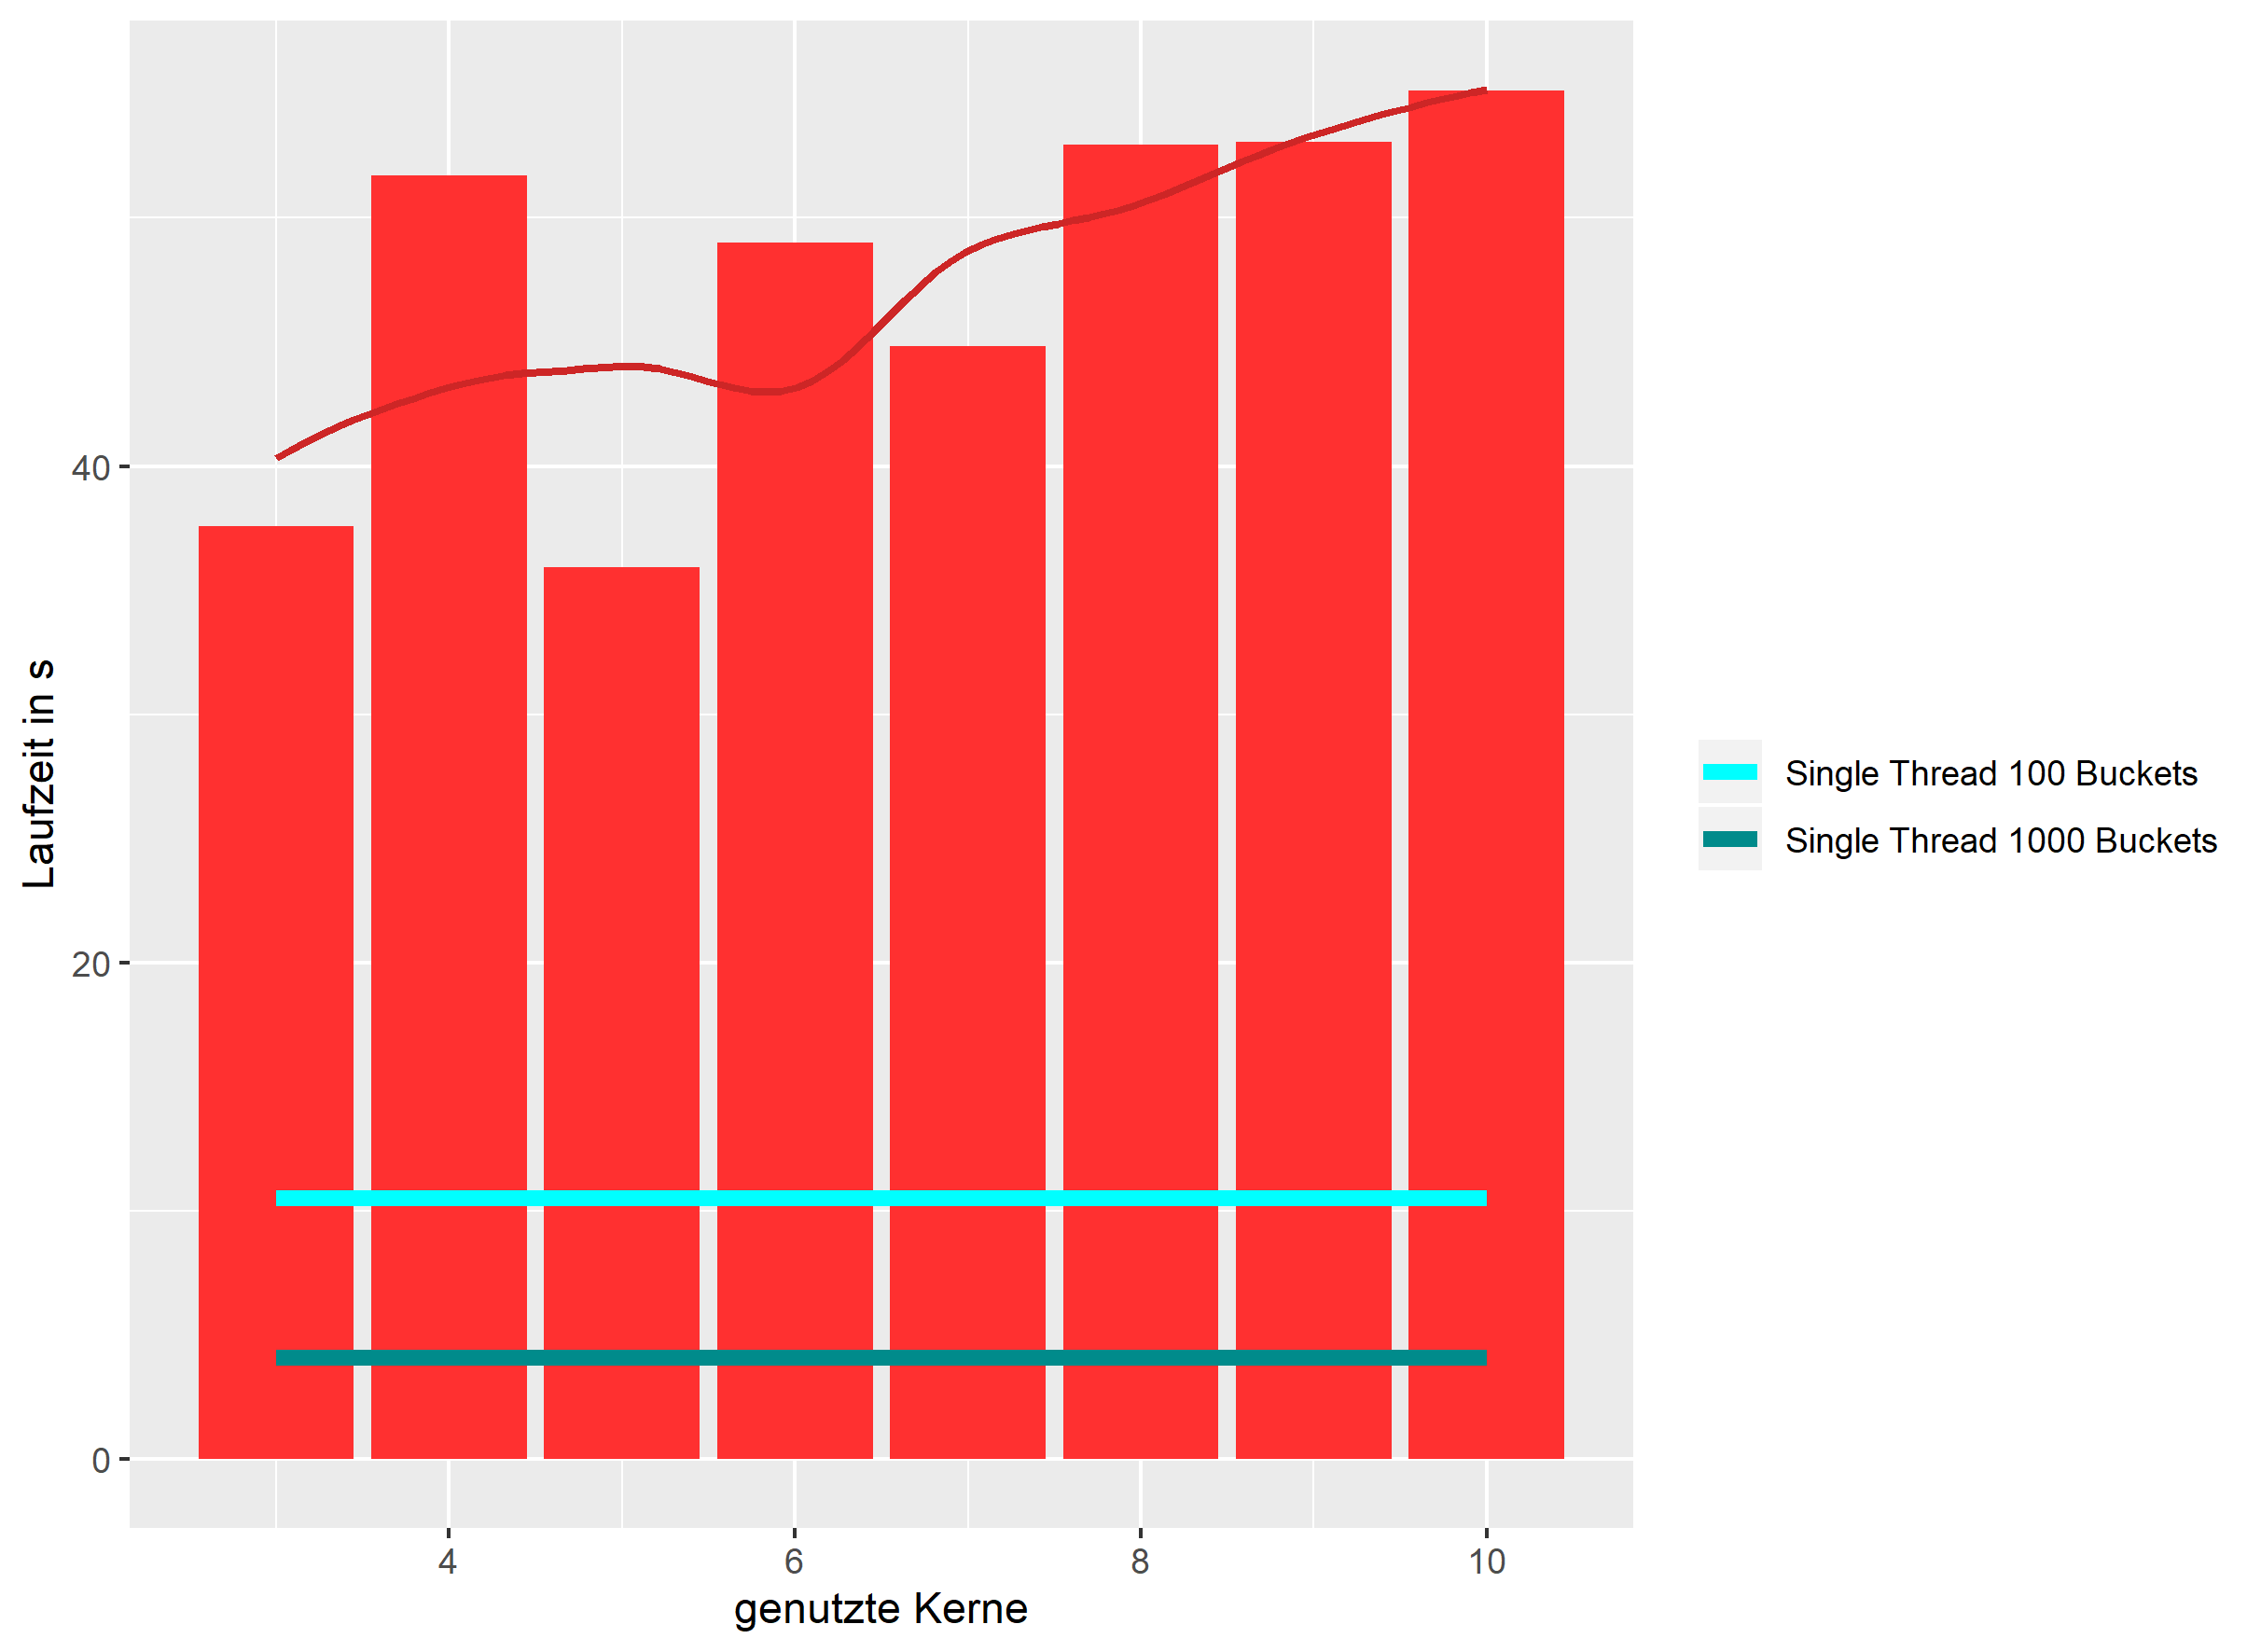
\includegraphics[width=0.7\textwidth]{Bilder/join_kerne_self.png}
	\caption{Laufzeitverhalten nach Kernen: Selfjoin der Relation \Fb{roads\_str}}
	\label{img:joinKern}
\end{figure}

\begin{figure}
	\centering
	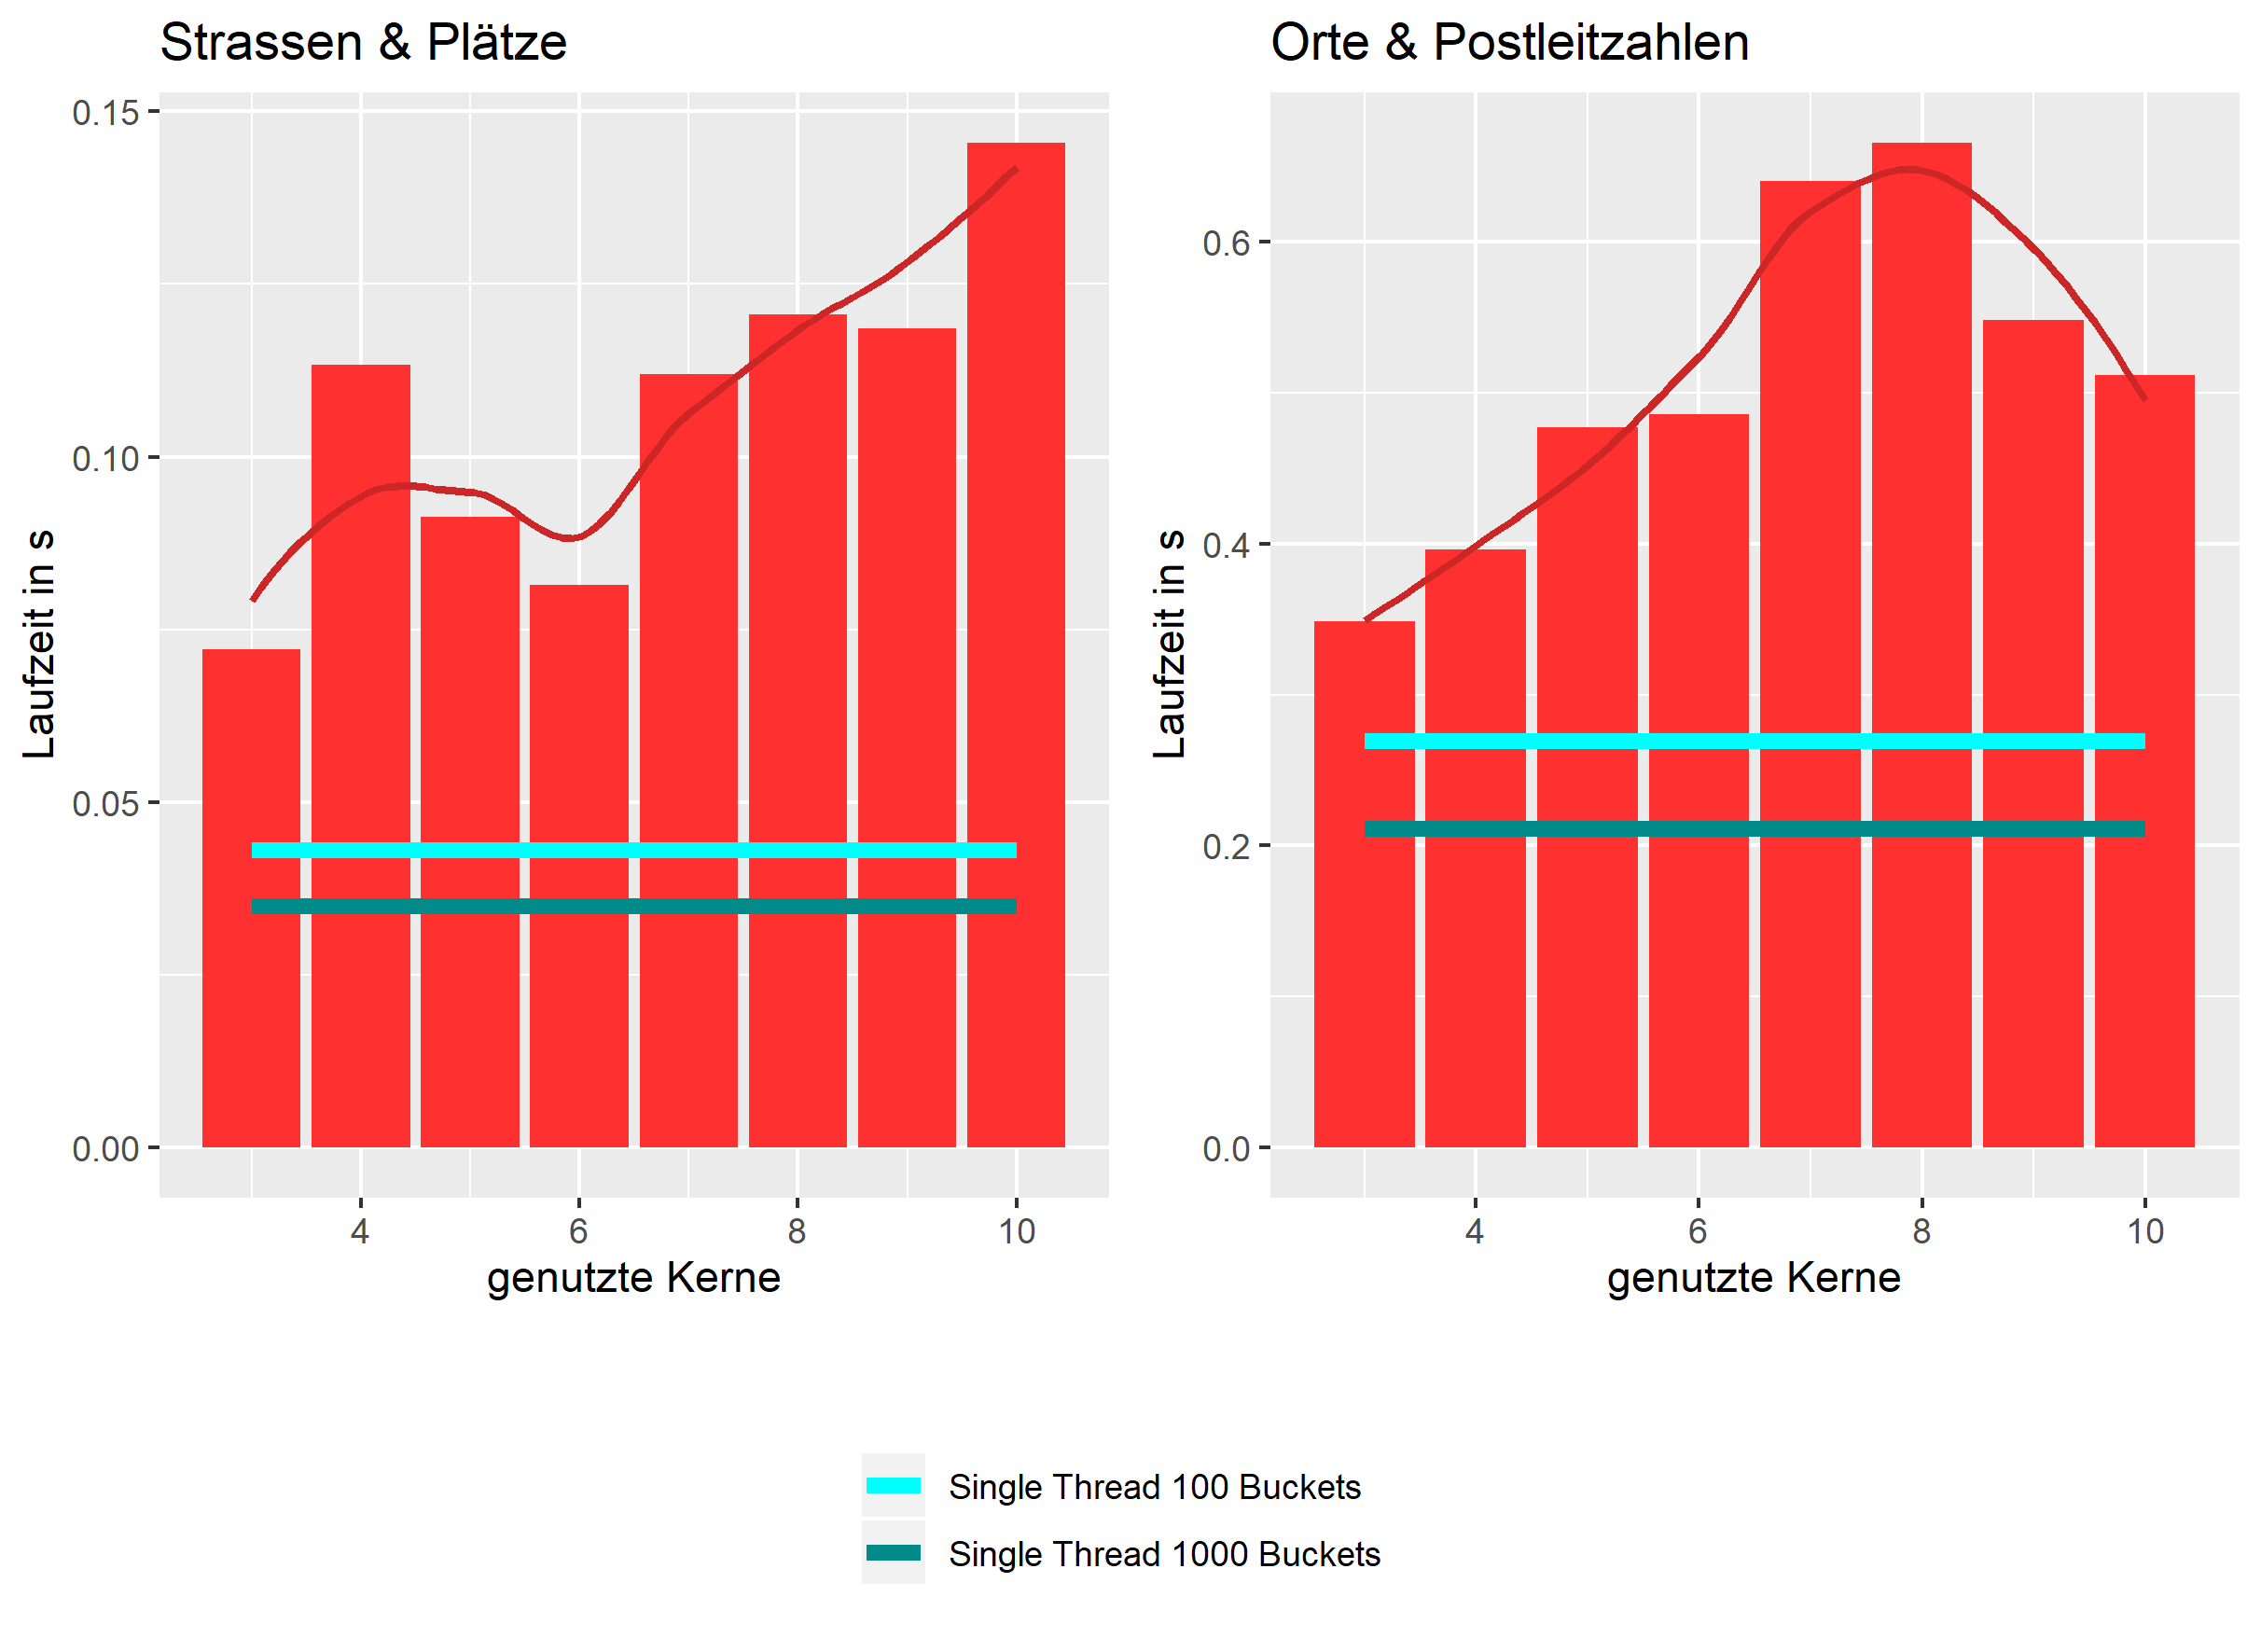
\includegraphics[width=0.7\textwidth]{Bilder/join_kerne_be.png}
	\caption{Laufzeitverhalten nach Kernen: Joins mit Relationen aus der \Fb{berlintest}-Datenbank}
	\label{img:joinKernBe}
\end{figure}

Aufwändig wird die Berechnung der Joins vor allem, wenn viele Tupel in das gleiche Bucket eingefügt werden, also den gleichen Hashwert haben. Wenn dadurch die Verteilung zwischen den Threads insbesondere für die aufwändigen Berechnungen sehr ungleich wird, verliert der Multithread-Operator Vorteile gegenüber dem Singlethread-Version. Beide Joins aus \autoref{img:joinKernBe} zeigen einerseits ein Verhältnis aus vergangener Zeit und CPU-Zeit \footnote{ca. 0,65 bei 3 Threads, sinkend mit Anzahl genutzter Kerne}, welches auf eine stärkere Parallelisierung als beim Join in \autoref{img:joinKern} \footnote{ca. 0,8, fast konstant bleibend bzgl. Anzahl der Kerne} hinweist. Für das schlechtere Laufzeitverhalten des Selfjoins gegenüber den beiden anderen Joins gäbe es zwei mögliche Erklärung: I/O-Zugriffe, die nicht parallelisiert werden können oder eine ungünstige Verteilung auf die Hashtabellen und Threads.

Dagegen verschlechtert sich der Laufzeitverhalten der beiden Joins insgesamt kleinerer Relationen deutlich stärker mit der Anzahl genutzter Kerne. Da beide R-Relationen deutlich kleiner sind als \Fb{roads\_str}, liegt das wahrscheinlich vor allem daran, dass die Relation zu klein sind für die in meiner Implementierung gewählten Entwurf eines Hybrid-Hash-Joins. Dagegen habe ich für den Selfjoin bereits im letzten Abschnitt erläutert, warum er kein gutes Parallisierungsverhalten zeigt. 

\subsubsection{Funktionstest MThreadedSpatialJoin}

Der Selbsttest des Spatial-Join-Operator zeigt mit der Option \Fb{--valgrindlc} auch bei großen Relationen kein Speicherleck.

\begin{minipage}{\linewidth}
	\begin{lstlisting}[caption={Beispiel Testqueries für den Spatial-Join-Operator ohne \Fb{project} und \Fb{sortby}}, label=list:testspatialjoin]
	query (roads feed {o} natural feed {p} mThreadedSpatialJoin[Geometry_o, Geometry_p, 0.0]
	roads feed {o} natural feed {p} spatialjoin[Geometry_o, Geometry_p]
	roads feed  extend[ B : enlargeRect(bbox(.Geometry), 1.0, 1.0) ] {o} natural feed extend[ B : bbox(.Geometry)] {p} symmjoin[.B_o intersects ..B_p]
	\end{lstlisting}
\end{minipage}

Zeile 1 in \autoref{list:testspatialjoin}) zeigt den Aufruf des Operators. Der Test auf Korrektheit muss sicherstellen, dass jeder Programmteil des Operators durchlaufen wird. Deswegen wird mit unterschiedlich großen Relationen und einer Begrenzung des Arbeitsspeichers getestet. Zusätzlich habe ich mir die Anzahl der Iterationen über S ausgeben lassen, um zu beobachten, inwieweit Teile von Relationen ausgelagert wurden. Duplikate können nur bei Attributen auftreten, die eine räumliche Ausdehnung haben. Zum Test der Duplikatseliminierung wird deswegen mit Attributen des Typs \Fb{Region} und vielen Kernen, und damit vielen Partitionen, getestet, um Duplikate wahrscheinlich zu machen. Verglichen werden die Ergebnisse mit dem Single-Thread Spatial-Join-Operator (Zeile 2 in \autoref{list:testspatialjoin}). Da eine gleiche Sortierung der Ergebnisrelation nicht garantiert werden kann, wird vor dem Vergleich die Ergebnisrelation auf die beiden Attribut \Fb{Name} der Eingangsrelationen projiziert und sortiert. Für den Test der Korrektheit der Option, die eine Vergrößerung der \Fb{MBB}, musste als Vergleich der \Fb{symmjoin}-Operator genutzt werden, dessen Eingangsstrom um die vergrößerte MBB ergänzt wurde (Zeile 3 in \autoref{list:testspatialjoin}). \autoref{tab:testSpatial} gibt eine Übersicht über die gemachten Tests, die alle fehlerfrei verliefen. In der Spalte \Fb{speicherintern} ist die Anzahl der Iterationen dargestellt. 

\begin{table}
	\centering
	\begin{tabular}{|c|c|c|c|c|}
		\hline 
		Relationen & Threads & speicherintern & Typ Join-Attribute & Tupel Ergebnisrelation \\ 
		\hline 
		$pois \bowtie traf$ & 3 & ja & Point \& Point & true \\ 
		\hline 
		$pois \bowtie roads$ & 3 & ja & Point \& Line & true \\ 
		\hline
		$pois \bowtie places$ & 3 & ja & Point \& Region & true \\ 
		\hline
		$roads \bowtie waterways$ & 3 & ja & Line \& Line & true \\ 
		\hline
		$roads \bowtie landuse$ & 3 & ja & Line \& Region & true \\ 
		\hline
		$landuse \bowtie natural$ & 3 & ja & Region \& Region & true \\ 
		\hline
		$roads \bowtie natural$ & 3 & ja & Line \& Region & true \\ 
		\hline
		$roads \bowtie natural$ & 6 & ja & Line \& Region & true \\ 
		\hline
		$roads \bowtie natural$ & 6 & nein & Line \& Region & true \\ 
		\hline
		$roads \bowtie natural$ & 6 & nein & Line \& Region & true \\ 
		resize MBB 1.0 &  &  &  &  \\ 
		\hline
	\end{tabular}
	\caption{\label{tab:testSpatial}Korrektheit Spatial Join}
\end{table}
  
\begin{table}
	\centering
	\begin{tabular}{|c|c|}
		\hline 
		Test & Ergebnis \\ 
		\hline
		R-Relation leer & leere Ergebnisrelation \\ 
		\hline
		S-Relation leer & leere Ergebnisrelation \\ 
		\hline
		R- \& S-Relation leer & leere Ergebnisrelation \\ 
		\hline
		R-Relation 2 Tupel & leere Ergebnisrelation \\ 
		\hline
		R kein Strom & first arg is not a tuple stream \\ 
		\hline
		S kein Strom & second arg is not a tuple stream \\ 
		\hline
		Join-Attribut R nicht räumlich & first attribute not spatial \\ 
		\hline
		Join-Attribut S nicht räumlich & second attribute not spatial \\ 
		\hline
		Join-Attribut R nicht Teil von R & Geometry\_p is not an attribute of the first stream \\ 
		\hline
		Join-Attribut S nicht Teil von S & Geometry\_o is not an attribute of the second stream \\ 
		\hline
		nur 1 Join-Attribut & Signatur expected \\
		\hline
		3 Join-Attribute &  Signatur expected \\
		\hline
		Resize nicht angegeben & Signatur expected \\ 
		\hline
		Resize string & last argument has to be real \\ 
		\hline
		$waterways \bowtie roads$ consume & gelegendlicher Absturz in consume \\
		\hline
	\end{tabular}
	\caption{\label{tab:testSpatialRobust}Robustheit Spatial Join}
\end{table}

Für eine Vielzahl unterschiedlicher Relationen und deren Kombinationen wurde bereits auf Korrektheit getestet. Auch funktioniert der Operator sehr gut mit großen Relationen, wobei es inbesondere bei der Nutzung vieler Threads und bei sehr kleinen R-Relationen gelegentlich zu abstürzen bei der Beendigung der Abfrage kommt -- hier vermute ich ein Problem mit einer fehlenden Synchronisierung bei Zugriffen auf die Berkelely-DB. Problematisch kann es sein, wenn die Eingangsströme entweder ganz leer sind oder so wenige Tupel enthalten, dass eine Partitionierung auf alle Threads nicht möglich ist. Darüber hinaus wird getestet, ob im Type-Mapping Parameter zurückgewiesen werden, die für einen Spatial Join nicht sinnvoll sind. Die vorgenommenen Robustheitstest werden in \autoref{tab:testSpatialRobust} dargestellt, wobei die Tests immer bei der Verwendung von 6 Kernen und mit den beiden Relationen \Fb{roads} sowie \Fb{natural} ausgeführt worden sind. Zusätzlich wurden verschiedene komplexe Abfragen getestet. In Kombination mit dem \Fb{Consume}-Operator kommt es gelegentlich zu Abstürzen, da dort scheinbar korrupte Daten ankommen. Vermutlich liegt dieses Problem auch an den Problemen mit parallelen Zugriffen auf die Berkeley-Datenbank, sofern \Fb{FLOBs} verarbeitet werden. Die anderen durchgeführten Test entsprachen aber den Erwartungen.

\begin{figure}
	\centering
	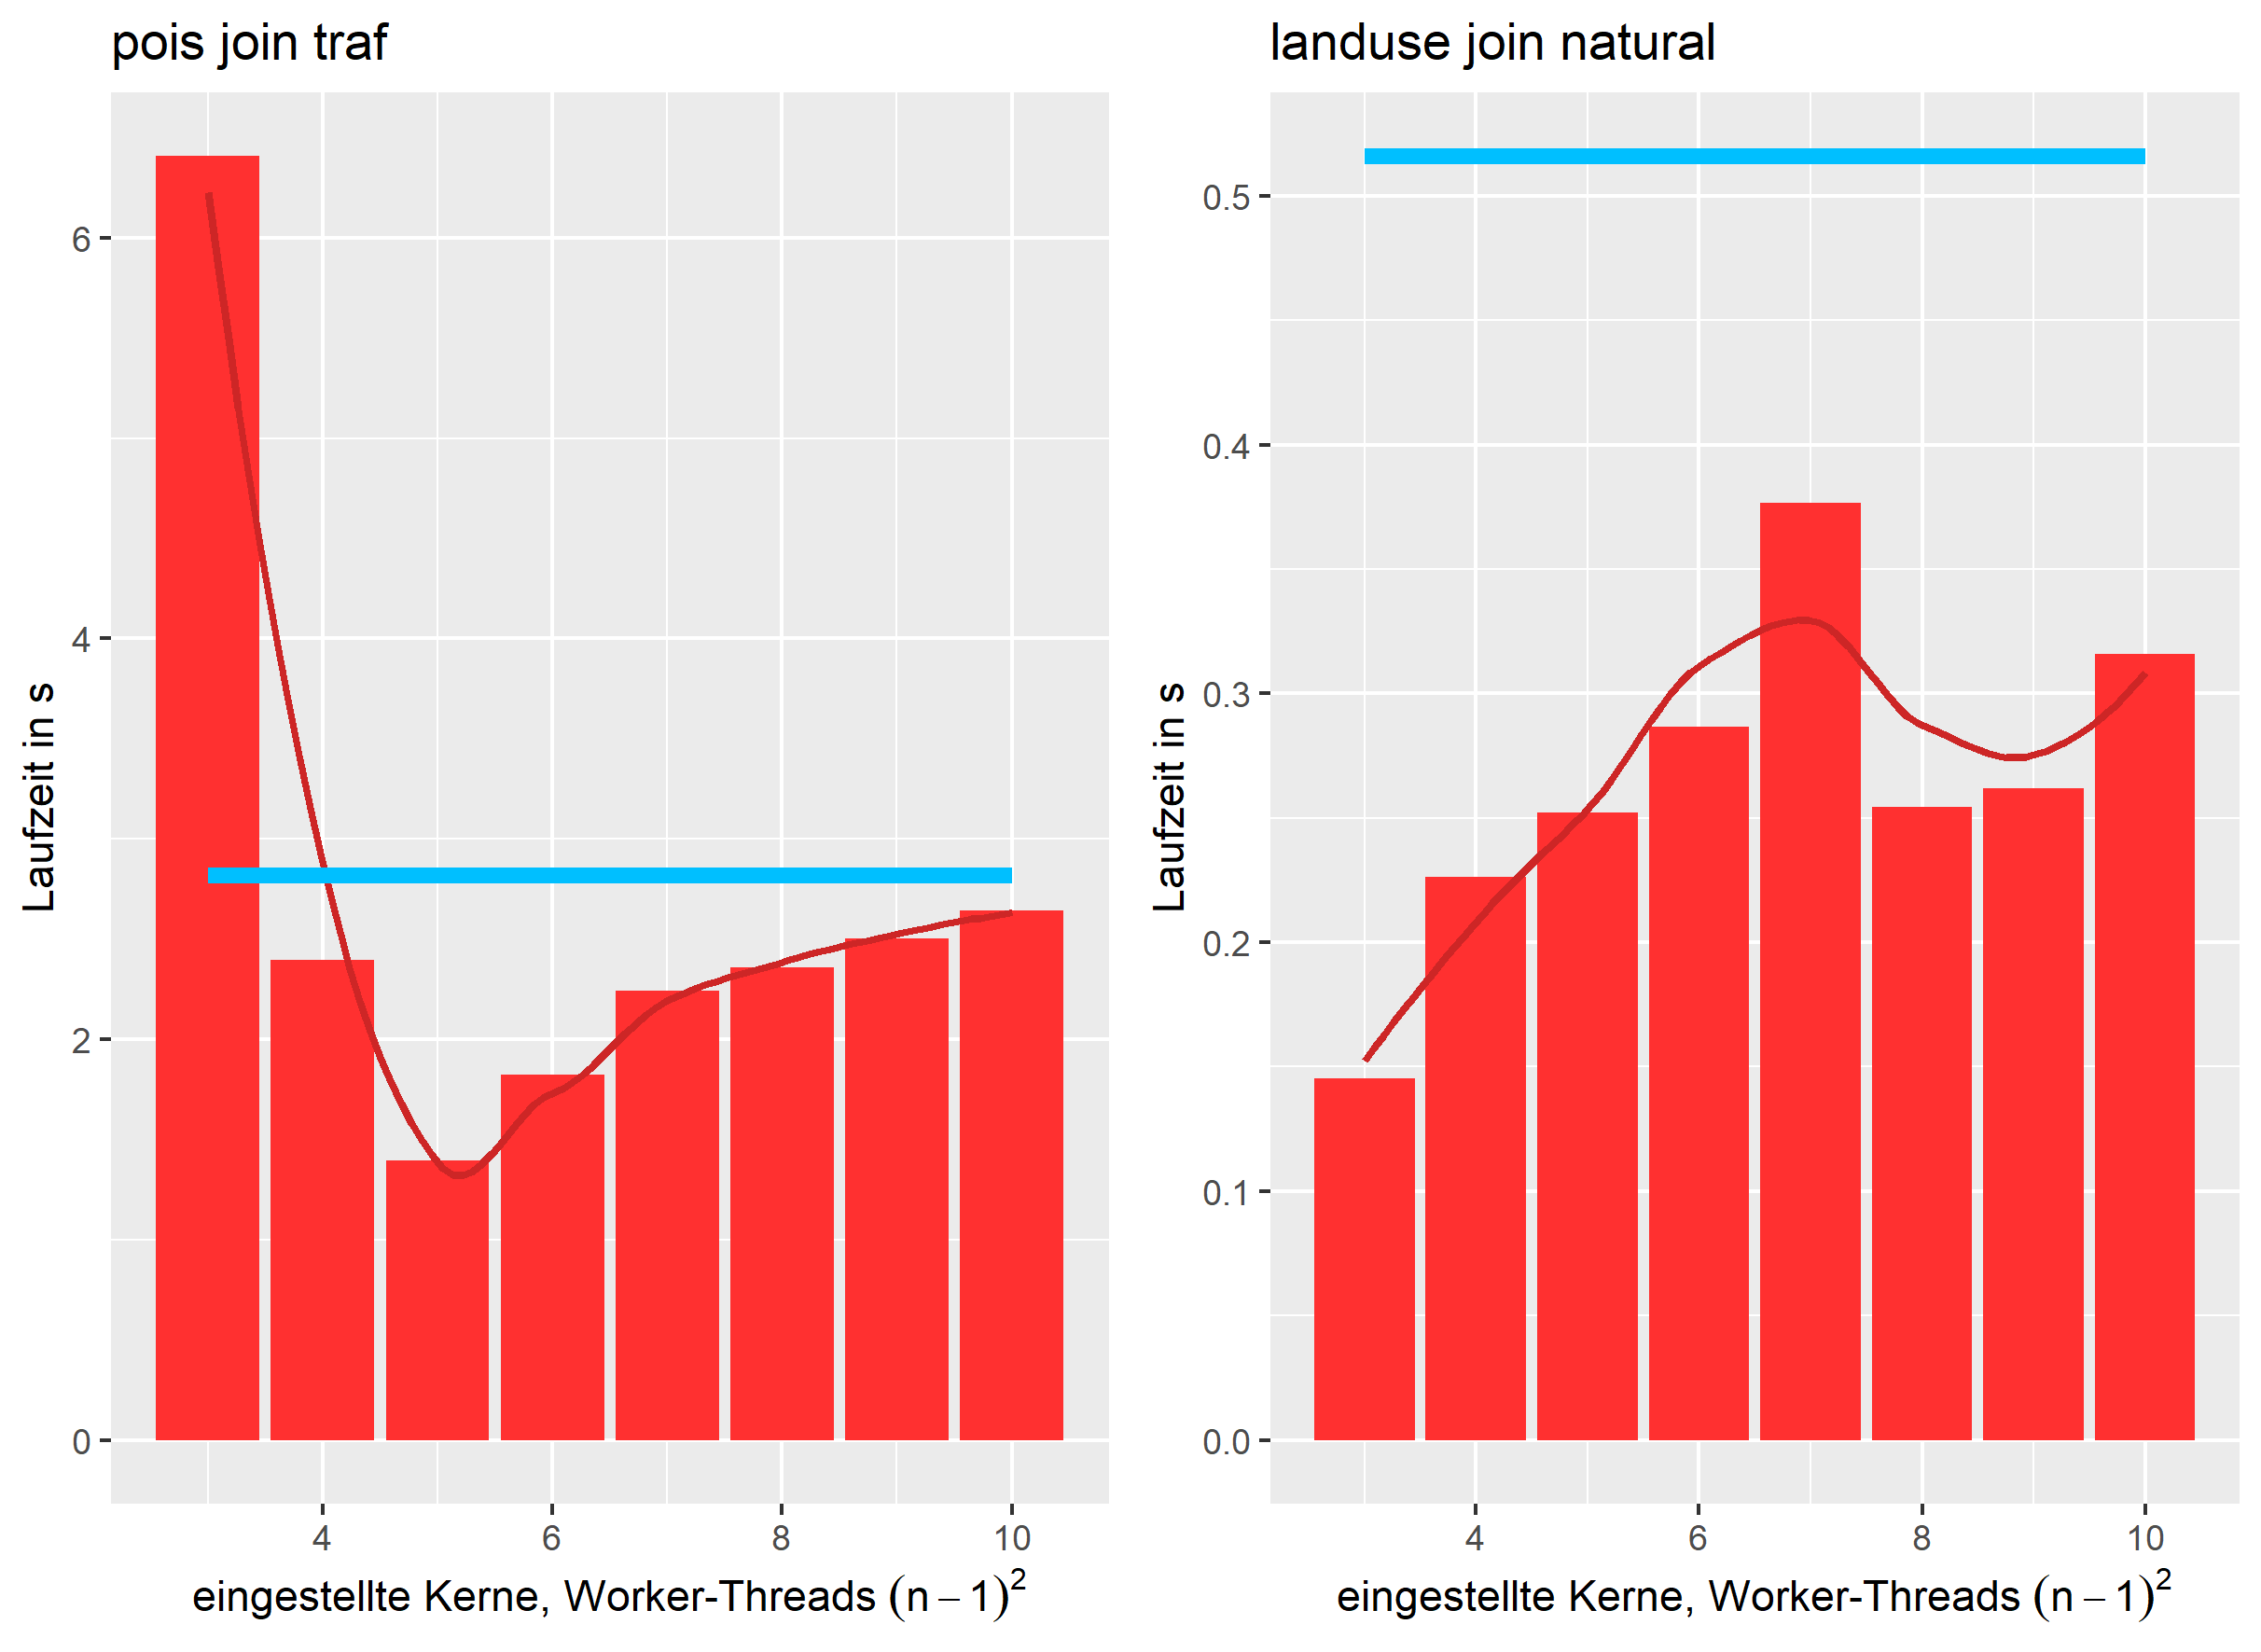
\includegraphics[width=0.70\textwidth]{Bilder/sj_kerne.png}
	\caption{Laufzeit zweier unterschiedlicher Spatial Joins im Vergleich mit der Single-Thread-Variante (blaue Linie).}
	\label{img:sjKern}
\end{figure}

\autoref{img:sjKern} zeigt das Laufzeitverhalten von zwei Spatial Joins. Die Relationen \Fb{landuse} und \Fb{natural} wurden auf 5.000 Tupel gekürzt und ergeben 1793 Ergebnistupel. Die beiden anderen Relationen, die über Punktattribute verschmolzen werden, haben nur eine Ergebnisrelation von 99 Tupeln, aber die Eingaberelationen sind beide groß (66.123 und 40.650 Tupel). In diesem Operator werden für $n$ konfigurierte Kerne $n^2$ Threads erzeugt, also meist mehr, als gleichzeitig möglich sind. Es hat sich herausgestellt, dass in diesem Fall der Operator ein wesentlich besseres Laufzeitverhalten hat (dieser Ansatz, deutlich mehr Partitionen zu erzeugen als Kerne zu verfügung stehen, hat den Operator teils um den Faktor 5 beschleunigt -- dieses Verhalten deutet die sehr schlechte Laufzeit bei $pois \bowtie traf$ mit $3^2$ Threads an). Mehr Threads zu nutzen als Kerne zur Verfügung stehen hat zu einer deutlich besseren Prozessornutzung geführt als in den anderen Operatoren -- der Koeffizient aus vergangener Zeit und CPU-Zeit liegt im Optimum bei den hier verwendeten Beispielanfragen bei 0,2 bzw. 0,3. Allerdings liegt das Optimum der Laufzeit nicht bei der maximalen Kernzahl, sondern bei $5^5$ bzw $3^3$ Threads, da für jeden Thread bei höherer Gesamtthreadtanzahl weniger Speicher zur Verfügung steht und die Eingangsströme nicht mehr direkt an die Threads durchgereicht werden können, sondern zwischengespeichert werden müssen. Bei größeren Relationen liegt das Optimum bei mehr Threads, da meine Implementierung einen nicht-linearen Anstieg der Rechenzeit im Bezug auf die Relationsgröße hat. Deutlich schneller als die Single-Thread-Version ist der Operator bei relativ kleinen Relationen.

Allgemein kann gesagt werden, dass die Multithread-Variante für die Beispielrelationen hier deutliche Geschwindigkeitsvorteile mit sich bringt, sofern eine optimale Kernzahl gewählt wird. Weitere Experimente in \autoref{exp:sj} zeigen allerdings, dass, wie hier bereits erwähnt, die Laufzeit mit der Relationsgröße exponentiell wächst, während die der Singlethread-Version nur linear ansteigt. Bei sehr großen Relationen und sehr vielen bestimmten Joinkandidaten ist der hier präsentierte Operator nicht mehr konkurrenzfähig.    


\subsubsection{Funktionstest MThreadedFilter}
\label{funk:filter}

\begin{minipage}{\linewidth}
	\begin{lstlisting}[caption={Testquery für den Filter-Operator, die auf Schnittpunkte zwischen Straßen und Wasserwegen prüft}, label=list:testfilter]
	query wr_sj feed mThreadedFilter[not(isempty(intersection_rob(.Geometry_o, .Geometry_p)));
	\end{lstlisting}
\end{minipage}

Der Filter-Operator hat keine komplexe Struktur, so dass in allen Fällen die zentralen Teilbereiche des Programms durchlaufen werden. Allerdings, wie bereits in \autoref{impl:refinement} diskutiert worden ist, gibt es Probleme mit der Synchronisation der Zugriffe auf die Berkeley-Datenbank, wenn die zu filternde Relation eine bestimmte Größe erreicht und in das Prädikat Attribute eingehen, die als \Fb{FLOBs} organisiert sind. Der Operator stürzt dann entweder im Commit ab oder gerät dort in einen Deadlock. Wenn Secondo ohne Commit gestartet wird, ist das Verhalten des Operators etwas stabiler, aber es treten auch Abstürze im Abschluss der Query-Ausführung auf oder teils auch beim Zugriff auf die  \Fb{FLOBs}.

\autoref{list:testfilter} zeigt beispielhaft eine Anfrage, die für den Korrektheitstest verwendet wurde. Verglichen wurde mit dem \Fb{filter}-Operator, der nur einen Kern nutzt. Die Ergebnisse der Tests zeigt \autoref{tab:testFilter}. Wenn in den Prädikaten keine Attribute mit \Fb{FLOBs} verwendet werden, liefert der Operator selbst bei sehr großen Relationen richtige Ergebnisse wie \autoref{tab:testFilter} zeigt.

\begin{table}
	\centering
	\begin{tabular}{|c|c|c|c|c|}
		\hline 
		Relationen & Prädikat & Relationsgröße & FLOB & Ergebnis \\ 
		\hline 
		buildings & $.Code > 1200$ & 502.309 & nein & true \\ 
		\hline 
		tp\_sj \footnotemark & $not(isempty$ & 99 & nein & true \\
		 & $(intersection1(.Geometry\_p, .Geometry\_o))$ &  &  &  \\ 
		\hline
		n2p\_sj \footnotemark & $not(isempty$ & 219.785.156
		 & nein & true \\
		& $(intersection1(.Geometry\_p, .Geometry\_o))$ &  &  &  \\ 
		\hline
		wr\_sj \footnotemark & $not(isempty$ & 1.000 & ja & true \\ 
		 & $(intersection1(.Geometry\_p, .Geometry\_o))$ &  &  &  \\ 
		\hline
		wr\_sj  & $not(isempty$ & 5.000 & ja & true \\
		 & $(intersection1(.Geometry\_p, .Geometry\_o))$ &  &  &  \\  
		\hline
		pl\_sj \footnotemark & $.Geometry\_o overlaps .Geometry\_p$ & 2.000 & ja & true \\ 
		\hline
		pl\_sj  & $.Geometry\_o overlaps .Geometry\_p$ & 5.000 & ja & true \\ 
		\hline
		wr\_sj  & $not(isempty$ & 12.000 & ja & true \\
		 & $(intersection1(.Geometry\_p, .Geometry\_o))$ &  &  &  \\  
		\hline
	\end{tabular}
	\caption{\label{tab:testFilter}Korrektheit Spatial Join}
\end{table}

\footnotetext{Die Relation tp\_sj ist ein Spatial Join zwischen traf und pois.}
\footnotetext{Die Relation n2p\_sj ist ein Spatial Join zwischen natural2 und pois mit head[20.000] bei einer Vergrößerung der MBB um 0,1.}
\footnotetext{Die Relation wr\_sj ist ein Spatial Join zwischen waterways und roads.}
\footnotetext{Die Relation pl\_sj ist ein Spatial Join zwischen roads und pois.}

Robustheit teste ich nur für kleine Relationen bzw. für Relationen ohne \Fb{FLOBs}, da ab einer bestimmten Relationsgröße der Operator hier im Commit bzw. im Abschluss der Anfragebearbeitung abstürzt (\autoref{tab:testFilterRobust}). Alle Ergebnisse entsprechen den Erwartungen.

\begin{table}
	\centering
	\begin{tabular}{|c|c|}
		\hline 
		Test & Ergebnis \\ 
		\hline
		Eingangs-Relation leer & leere Ergebnisrelation \\ 
		\hline
		Prädikat nie wahr & leere Ergebnisrelation \\ 
		\hline
		Eingangs-Relation nur 1 Tupel & Ergebnisrelation 1 Tupel \\ 
		\hline
		Ergebnis des Prädikats nicht boolean & fun result is not a bool \\ 
		\hline
		Attribut in Prädikat nicht Teil der Relation &  Attr name Geometry\_x not found in attribute list  \\ 
		\hline
		Eingang kein Tupelstrom & first arg is not a tuple stream \\ 
		\hline
		Operator in Prädikat nicht existent &  fun corrupt  \\ 
		\hline
		Prädikat hat Tupelstrom als Ergebnis & fun corrupt \\ 
		\hline
		Prädikat mit \Fb{FLOBs}, Relation 30.000 Tupel & Absturz \\ 
		\hline
	\end{tabular}
	\caption{\label{tab:testFilterRobust}Robustheit Filter-Operator}
\end{table}

\begin{figure}
	\centering
	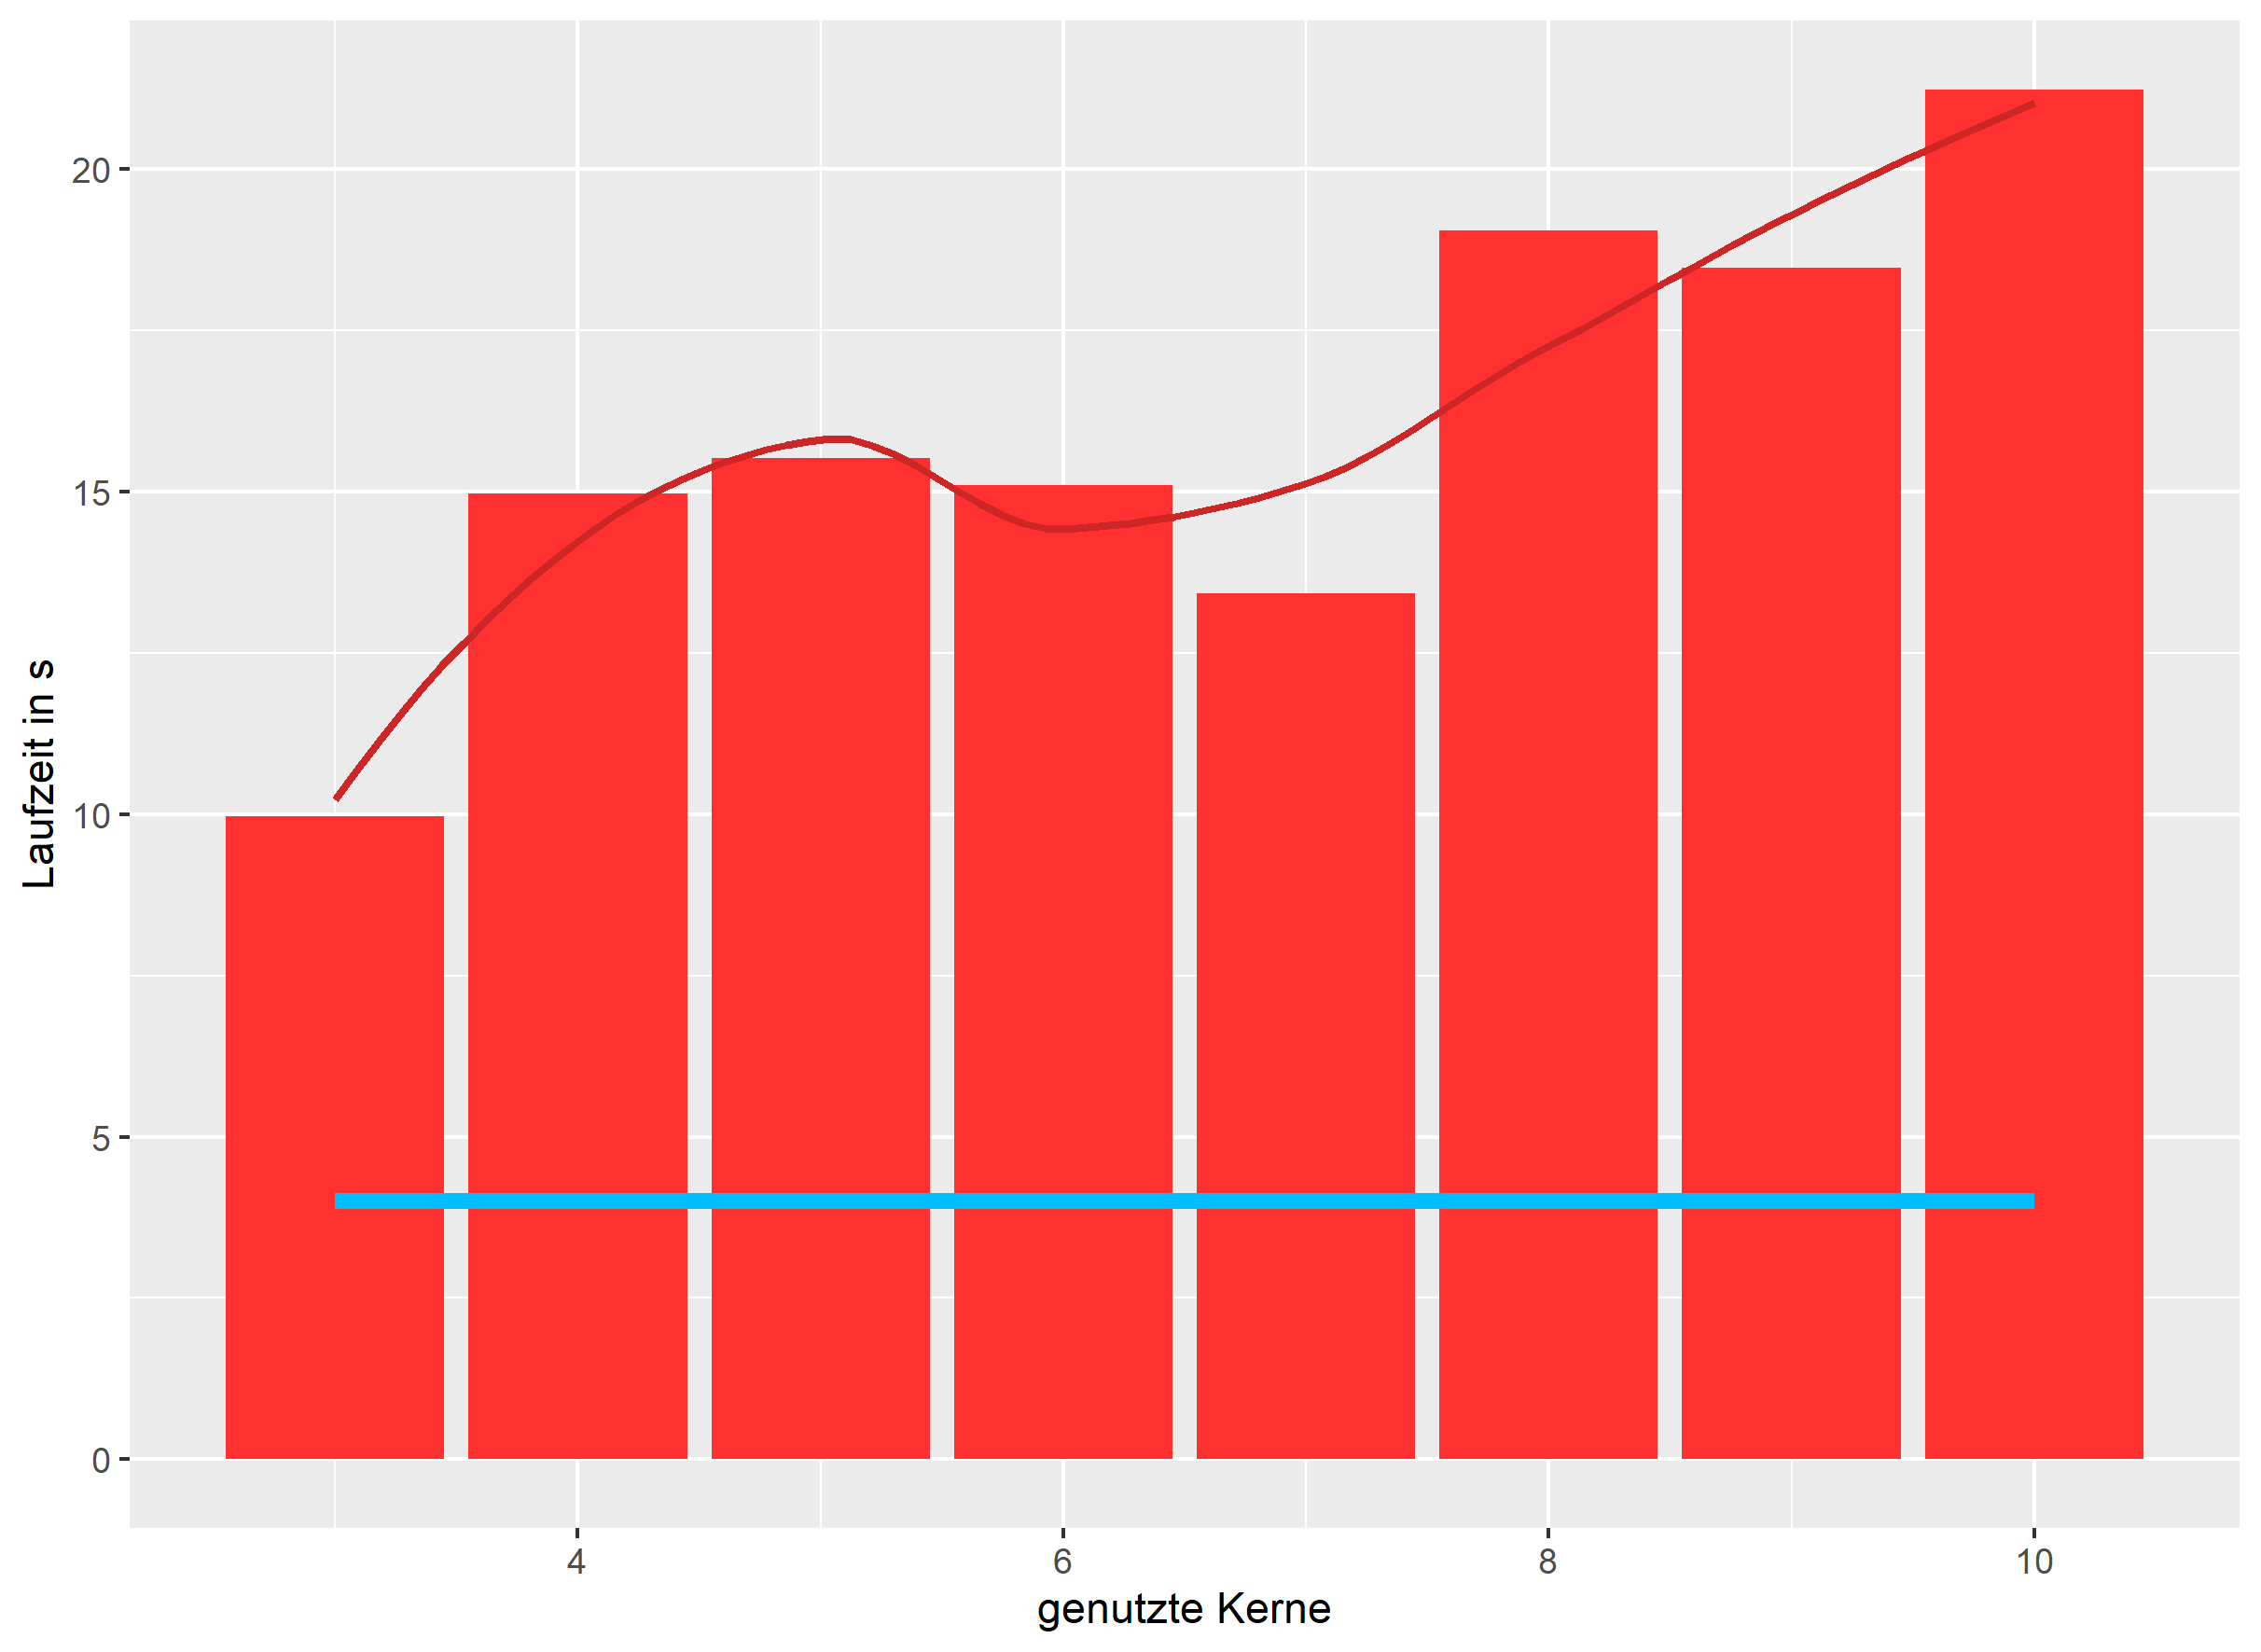
\includegraphics[width=0.65\textwidth]{Bilder/filter_kerne.png}
	\caption{Der Filter-Operator im Vergleich mit der Single-Thread-Variante (blaue Linie).}
	\label{img:filterKern}
\end{figure}

In seiner Effizienz ist der Filteroperator der \Fb{mThreaded}-Algebra deutlich schlecht als die Singlethread-Version (siehe \autoref{img:filterKern}). Analysiert habe ich den Filter \Fb{.Code > 1200} auf die Relation \Fb{buildings}. Bei der Nutzung von drei Kernen, also bei 2 Worker-Threads, ist die Multithread-Variante ungefähr halb so schnell wie die der Standard-Filter von Secondo. Tests mit komplexeren Prädikaten ergaben vergleichbare Ergebnisse. Eine Nutzung von mehr Kernen verschlechtert das Ergebnis zwar nicht linear, aber durchgehend. Auch bleibt die Parallelisierung quasi konstant bei steigender Kernzahl (Koeffizient aus verbrauchter Zeit und CPU-Zeit ist durchgehend bei knapp 0,7). Hier ist also eine durchgehende Nutzung mehrere Kerne nicht gelungen. Ursache kann eigentlich nur sein, dass durch die Synchronisierung entweder der Auswertungen in den Query-Prozessoren, der Queues für die Weitergabe der Eingangsströme bzw. Ergebnisse oder dem Wechsel zwischen Eingangsstrom- und Ausgangsstromweitergabe in der \Fb{getnext}-Methode Wartezeiten für Threads entstehen. Was diese Erkenntnis für Aussagen zulässt für die Effizienzprobleme fast aller Operatoren der  \Fb{mThreaded}-Algebra, diskutiere ich in \autoref{entw:filter} ausführlich.

\subsubsection{Experimente MThreadedsort}

Mit dem Multithread-Sortieroperator habe ich zwei Experimente vorgenommen, nämlich einen Vergleich des Laufzeitverhaltens bei steigender Tupelzahl in den Relationen für einfache Suchattribute und Mehrfach-Suchattribute sowie eine Untersuchung des Laufzeitverhaltens bei unterschiedlichem zur Verfügung stehendem Speicher und damit bei verschiedener Nutzung von Auslagerungsdateien.

\autoref{img:sortHeadExp} und \autoref{img:sortHeadMfExp} zeigen das Laufzeitverhalten am Beispiel der Sortierung der \Fb{buildings}-Relation nach der ID und der Relation \Fb{roads\-str} nach 6 Attributen, die so gewählt worden sind, dass für die Bestimmung der Reihenfolge meistens alle Attribute betrachtet werden müssen. Beide Verläufe zeigen, dass sich die Performance der Multithread-Variante mit der Relationsgröße gegenüber der Singlethread-Variante verschlechtert, allerdings in einem deutlich anderem Ausmaß. Während bei der Sortierung nach einem Attribut die Laufzeit exponentiell wächst, liegt bei vielen Sortierattributen, also wesentlich mehr Vergleichen innerhalb des Operators, ein lineares Wachstum vor, wenn auch mit einer stärkeren Steigung beim von mir implementierten Operator. 

\begin{figure}
	\centering
	\subfloat[nach Größe der Relation\label{img:sortHeadExp}]{{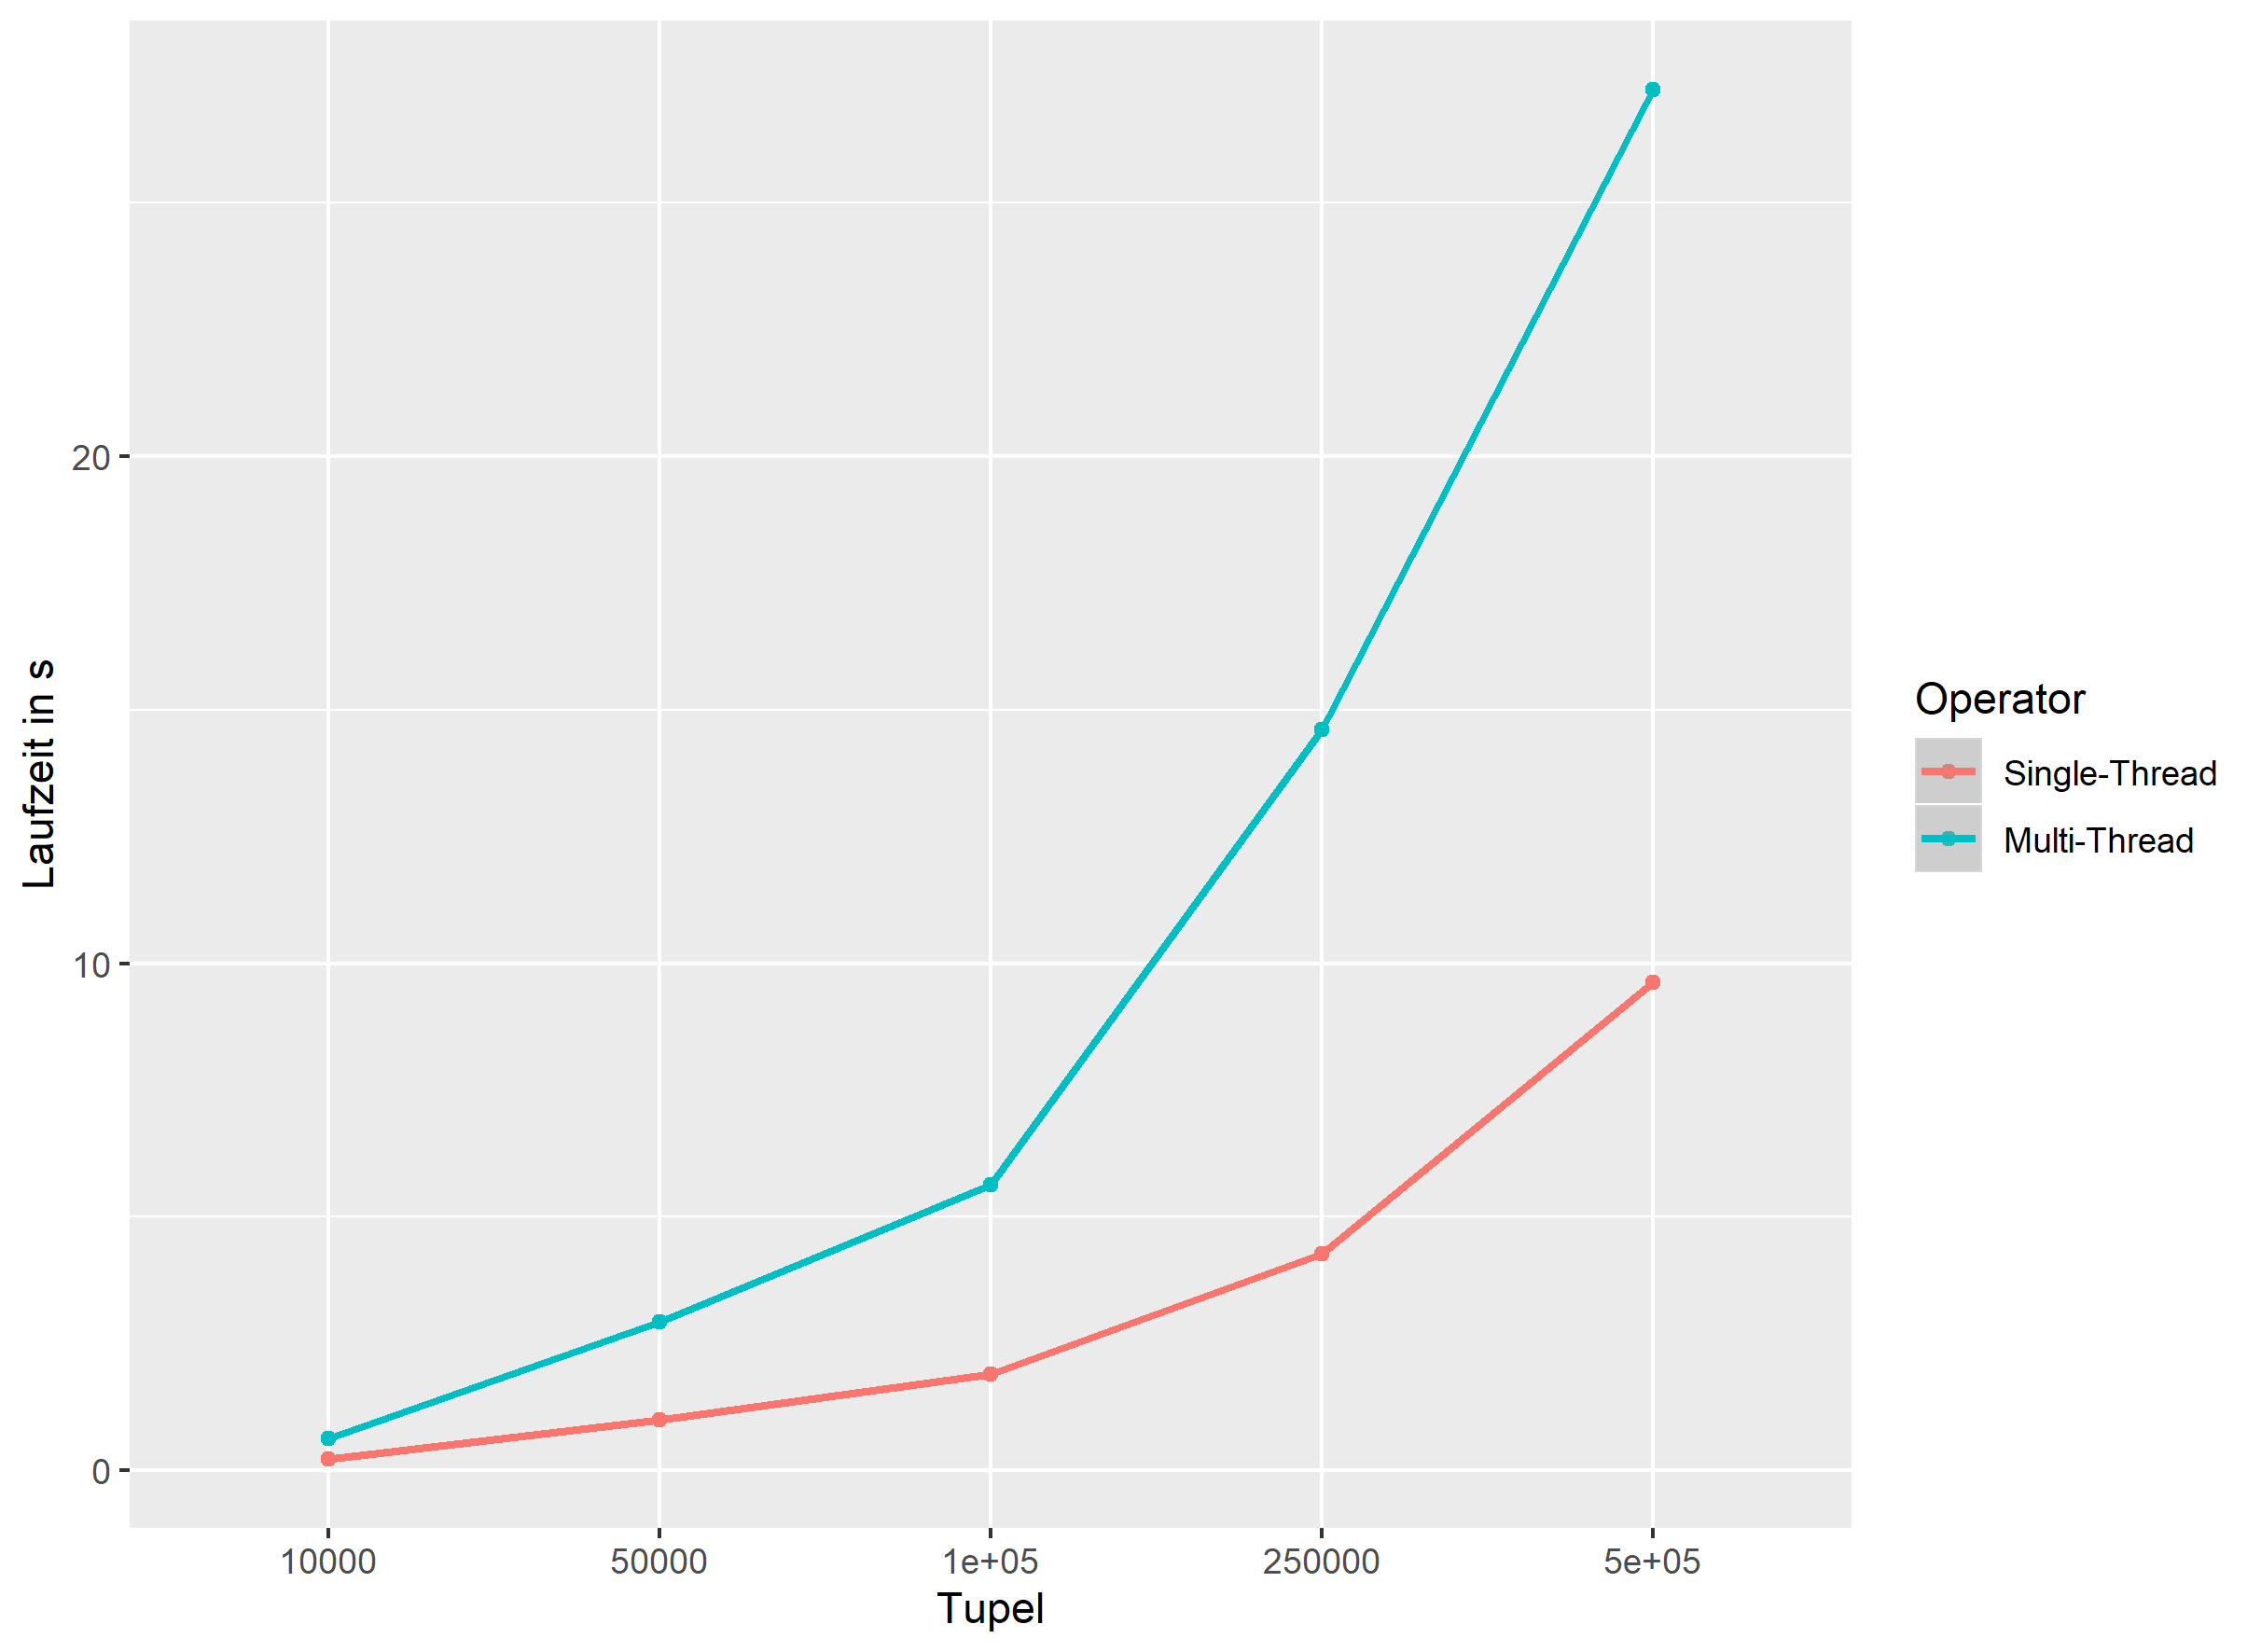
\includegraphics[width=0.45\textwidth]{Bilder/sort_head.png}}}
	\qquad
	\subfloat[zusätzlich mehrere Suchattribute\label{img:sortHeadMfExp}]{{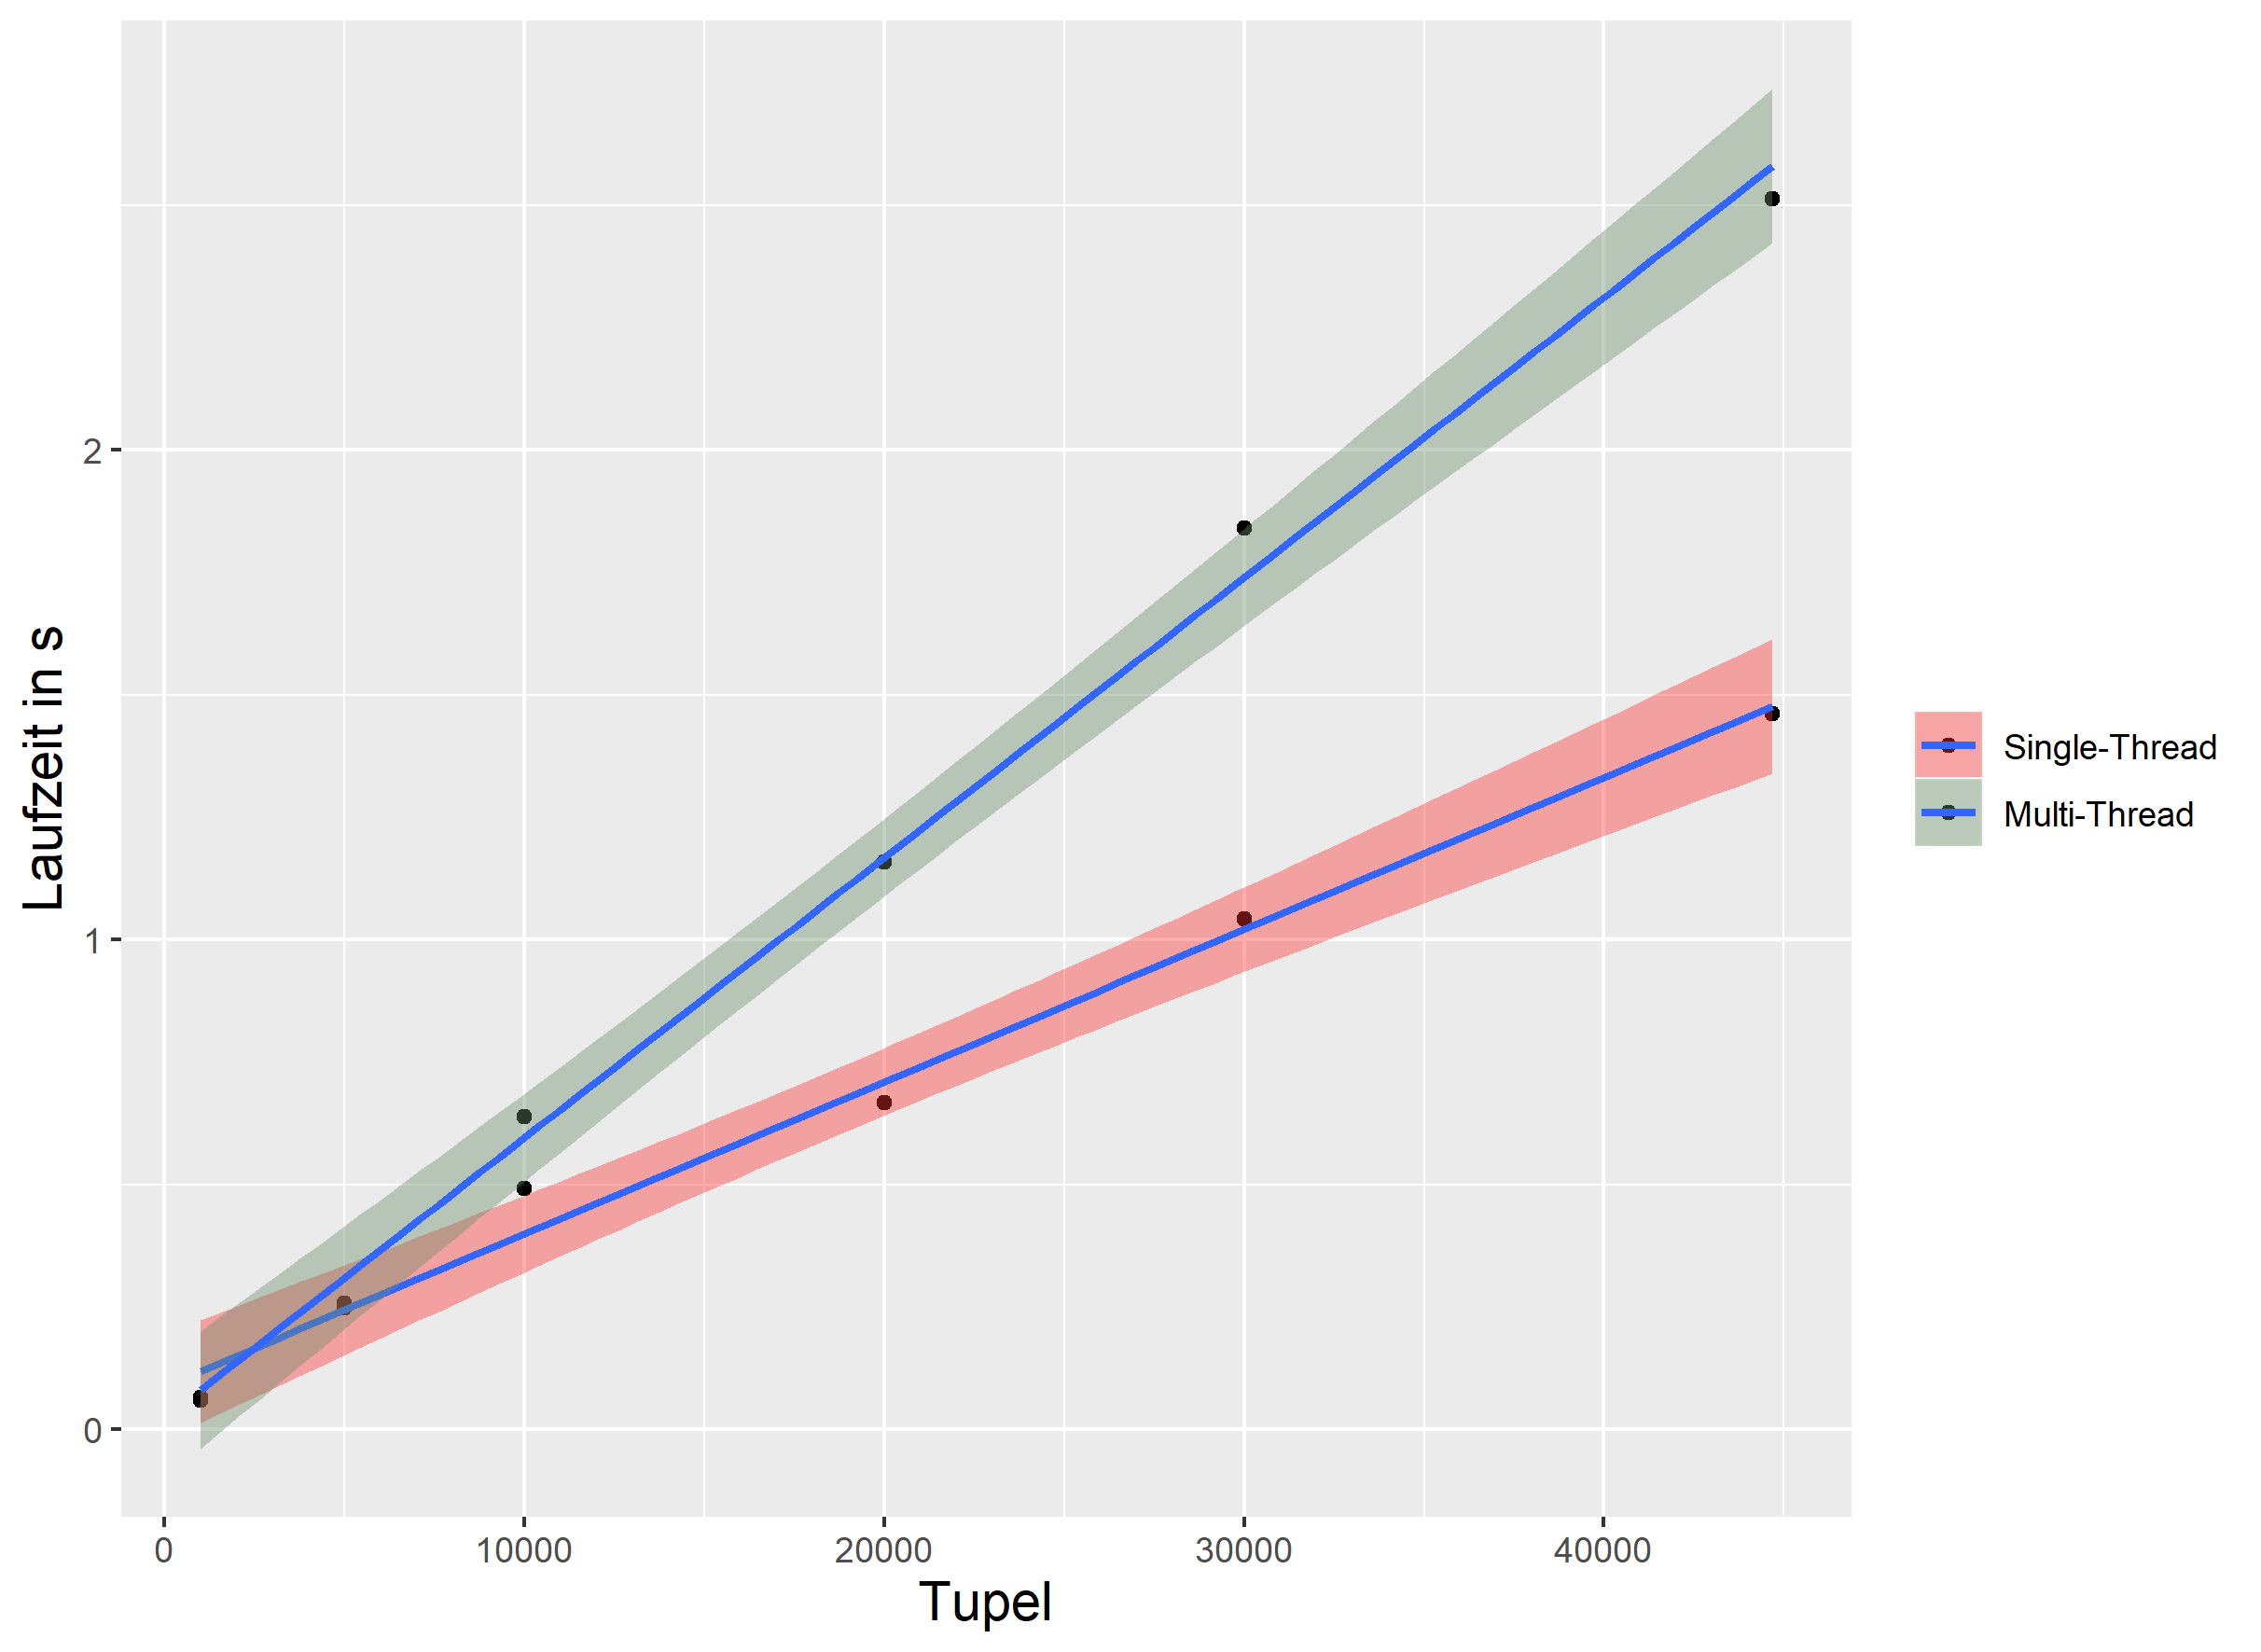
\includegraphics[width=0.45\textwidth]{Bilder/sort_head_mf.png}}}
	\qquad
	\subfloat[nach verfügbarem Speicher\label{img:sortMemExp}]{{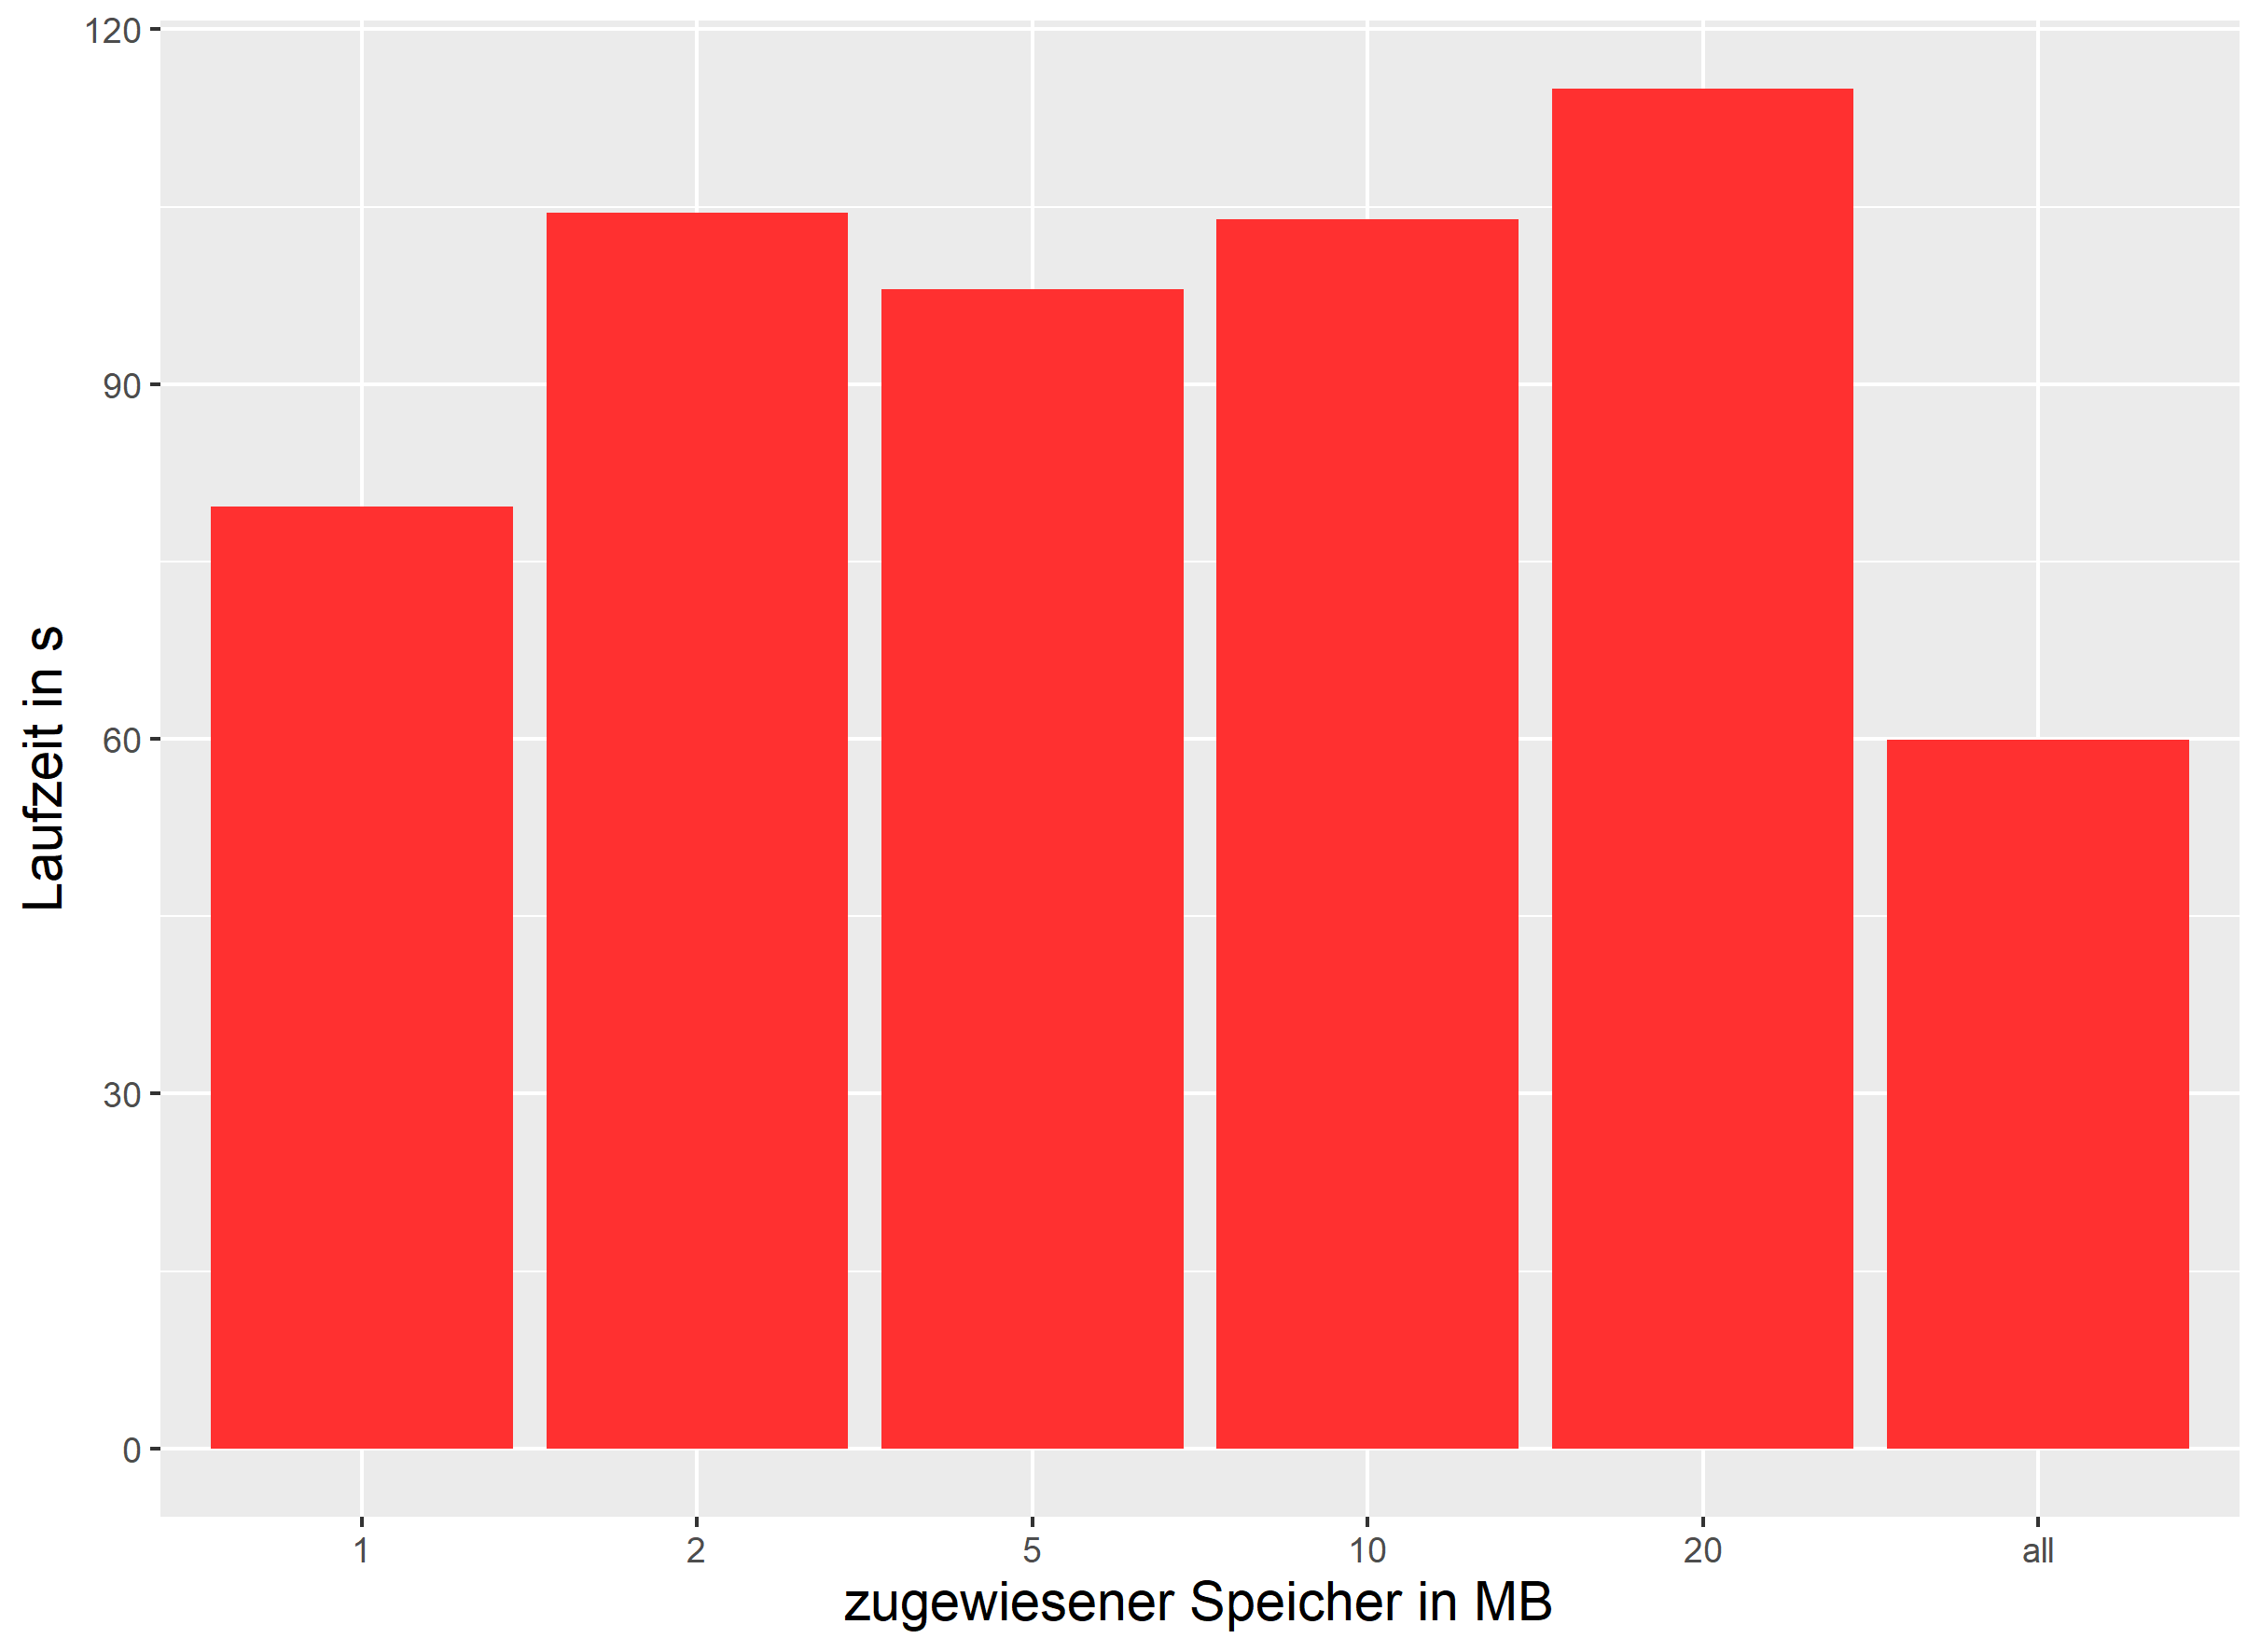
\includegraphics[width=0.35\textwidth]{Bilder/sort_mem.png}}}
	\caption{Experimente mit dem mThreadedMergeSort}
	\label{img:sortExpAllg}
\end{figure}

Der zur Verfügung stehende Speicherplatz für den Operator ist nur für die postoptimale Phase von Bedeutung und bestimmt, wieviel Läufe innerhalb dieser Phase generiert und verschmolzen werden müssen. \autoref{img:sortMemExp} zeigt die Laufzeit der Sortierung der Relation \Fb{buildings} nach der ID bei unterschiedlichem zur Verfügung stehendem Hauptspeicher. Deutlich ist der Sprung von 20 auf 40 MB. Hier nehme ich an, dass bei 40 MB keine Auslagerungsdateien mehr notwendig sind. Warum die Laufzeit bis20 MB mit kleinen Abweichungen ansteigt, liegt wahrscheinlich an einer ungünstigen Verteilung auf die Läufe oder aber an den Schwankungen, die bei der Laufzeitmessung möglich sind (vgl. \autoref{te}).


\subsubsection{Experimente MThreadedHashJoin}
\label{exp:hash}

Für den Hash-Join-Operator untersuche ich sein Verhalten gegenüber Änderungen des Speicherplatz, der ihm zur Verfügung steht, gegenüber der wachsender Tupelzahl in R- und S-Relation sowie wie sich die Konfigurierung der Hashtabellen auf sein Laufzeitverhalten auswirken \autoref{img:joinBucket}.

Eine Analyse, inwieweit sich die Performance des Operators sich verändert, wenn ihm unterschiedlich viel Speicherplatz zur Verfügung steht, wurde mit einem Selfjoin der Relation \Fb{roads\_str} vorgenommen \autoref{img:joinMemExp}. Wenn weniger Speicher zur Verfügung steht, bedeutet dies vor allem, dass Teile der Hashtabellen ausgelagert werden und evtl. ein rekursiver Aufruf des Verschmelzungs-Algorithmus notwendig wird. Dies ist allerdings vor allem dann der Fall, wenn die R-Relation bezüglich des Joinattributs sehr ungleich verteilt ist. Die Tendenz der Laufzeit bei steigendem zur Verfügung stehenden Speicher ist zwar deutlich abnehmend, aber die Abweichungen von der Regressionsgeraden sind sehr ausgeprägt. Deswegen gehe ich davon aus, dass, anders als erwartet, nicht mit Sicherheit festgestellt werden kann, dass eine Auslagerung von Buckets in Dateien eine große Auswirkung auf das Laufzeitverhalten hat.

\begin{figure}
	\centering
	\subfloat[Vergleich nach verfügbarem Speicherplatz\label{img:joinMemExp}]{{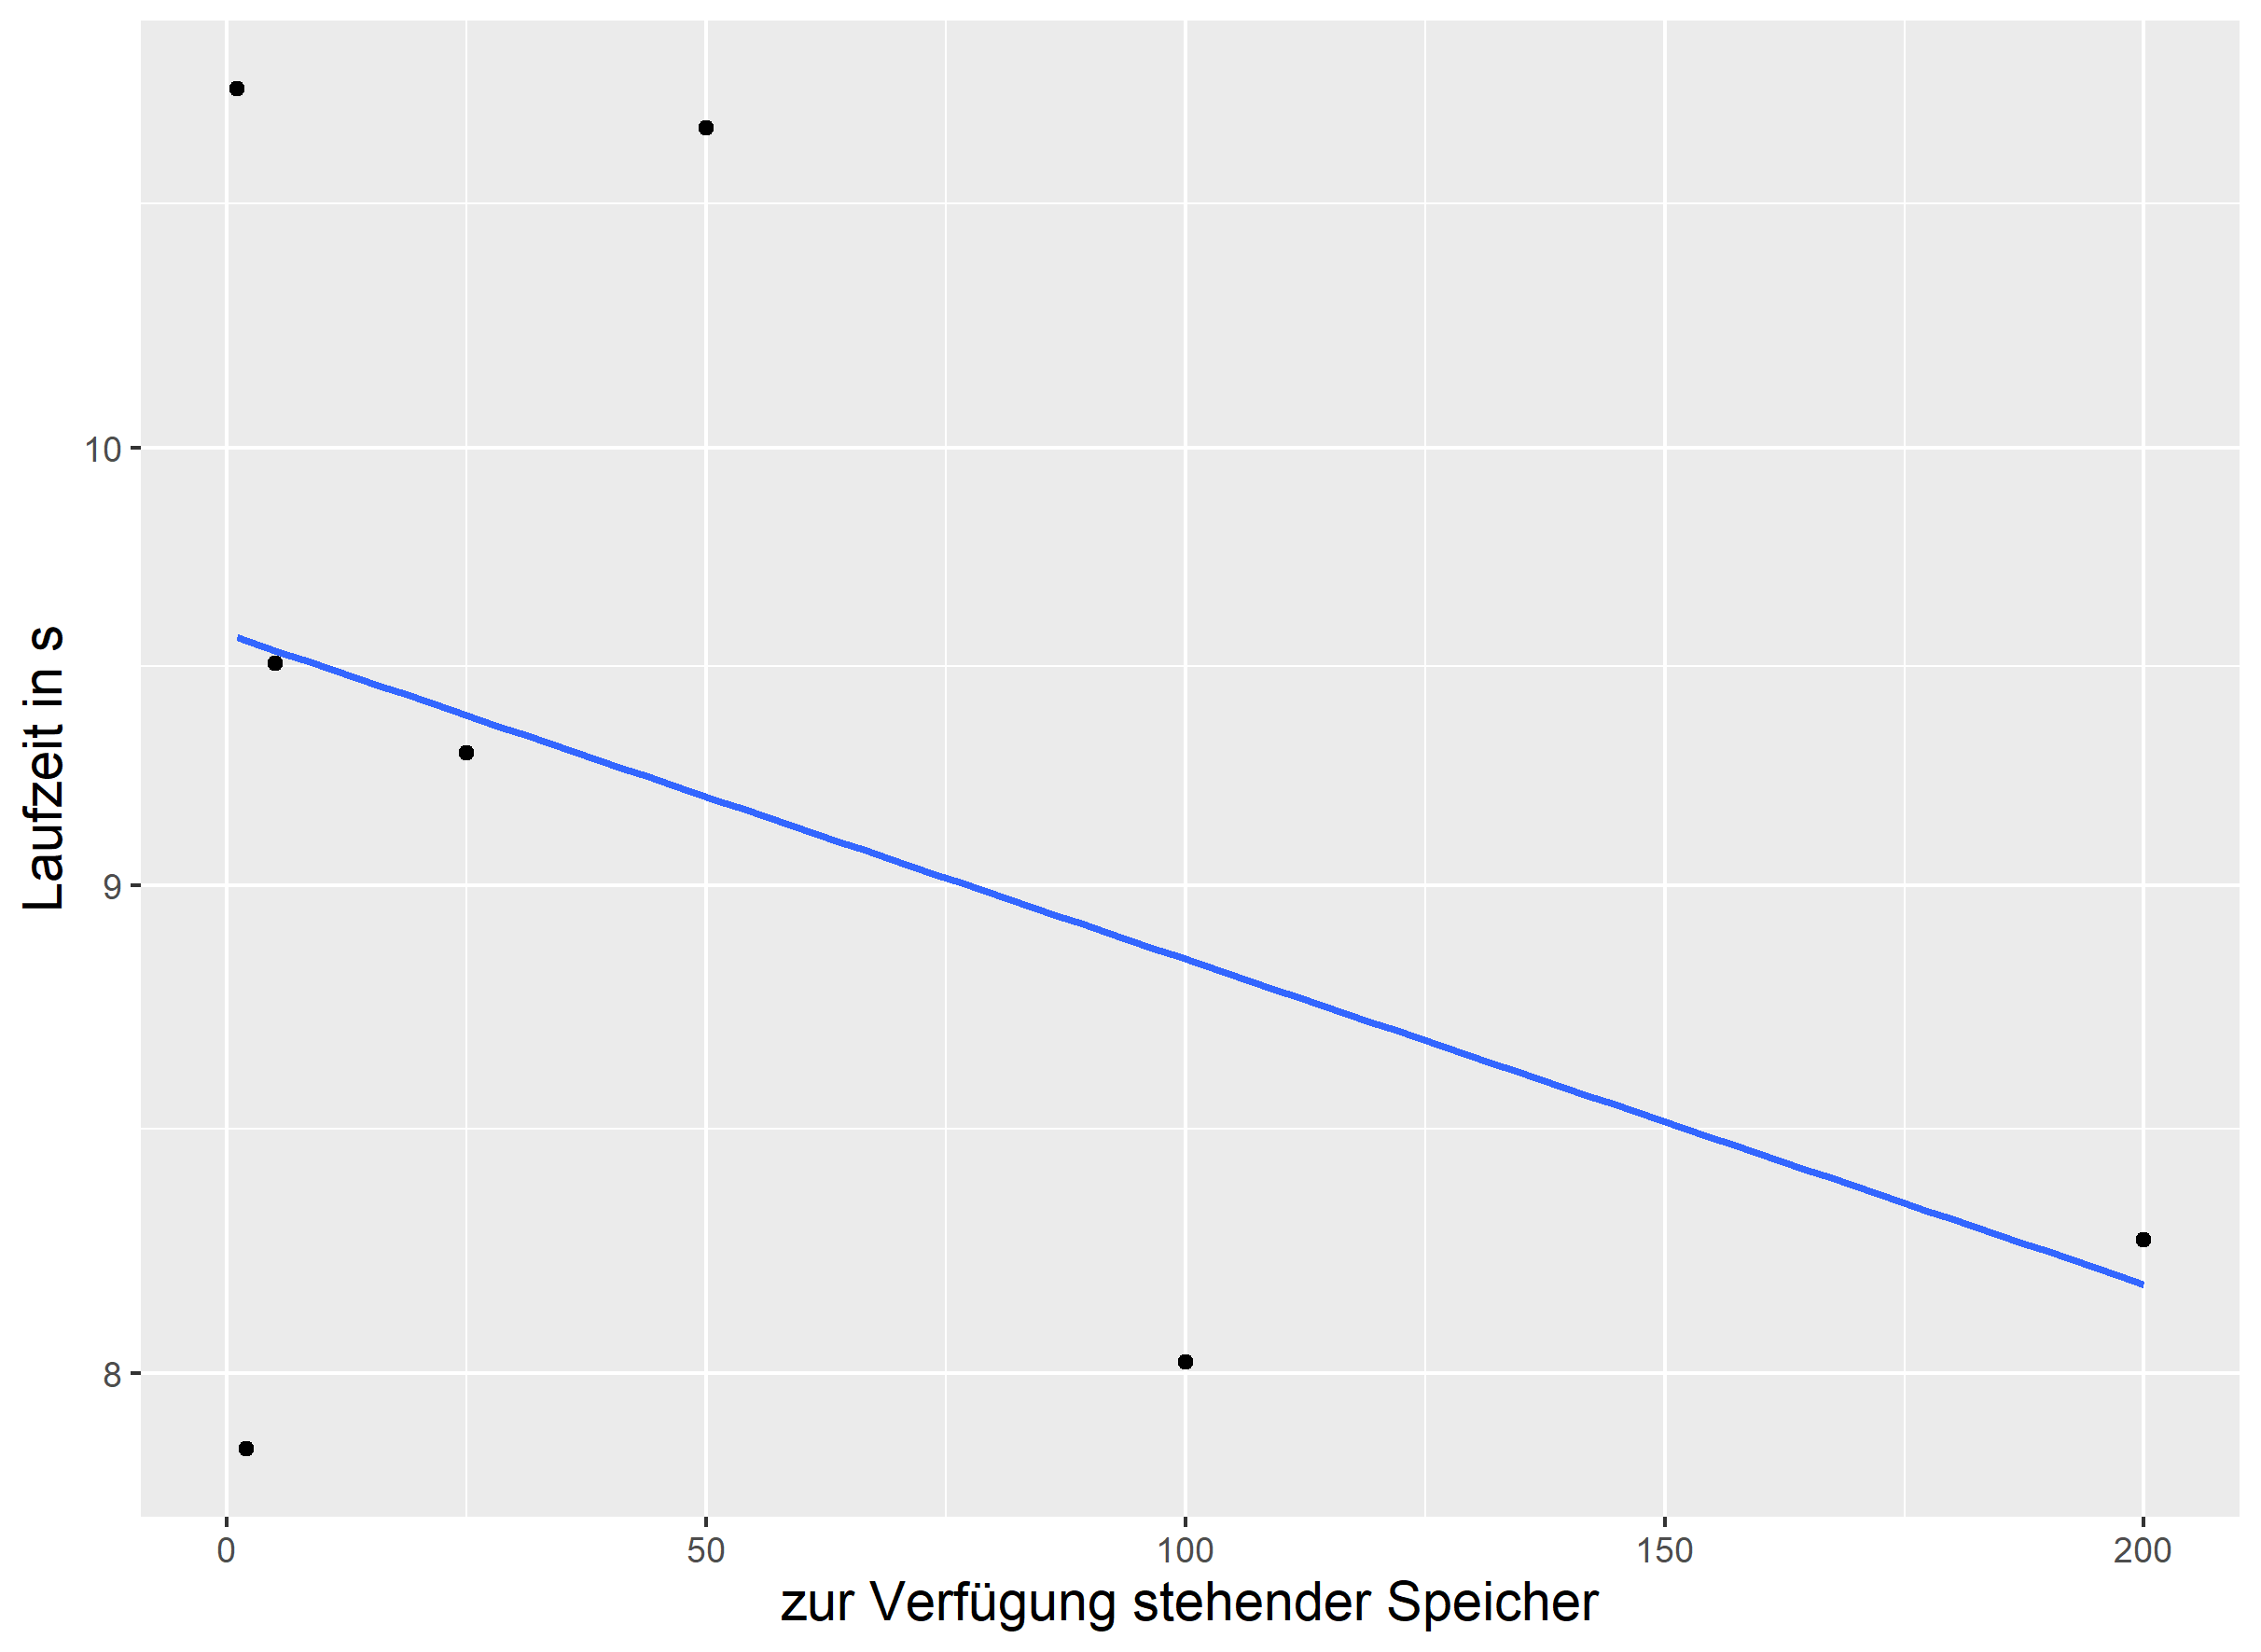
\includegraphics[width=0.45\textwidth]{Bilder/join_mem.png}}}
	\qquad	
	\subfloat[Vergleich nach Größe der Relation\label{img:joinHeadExp}]{{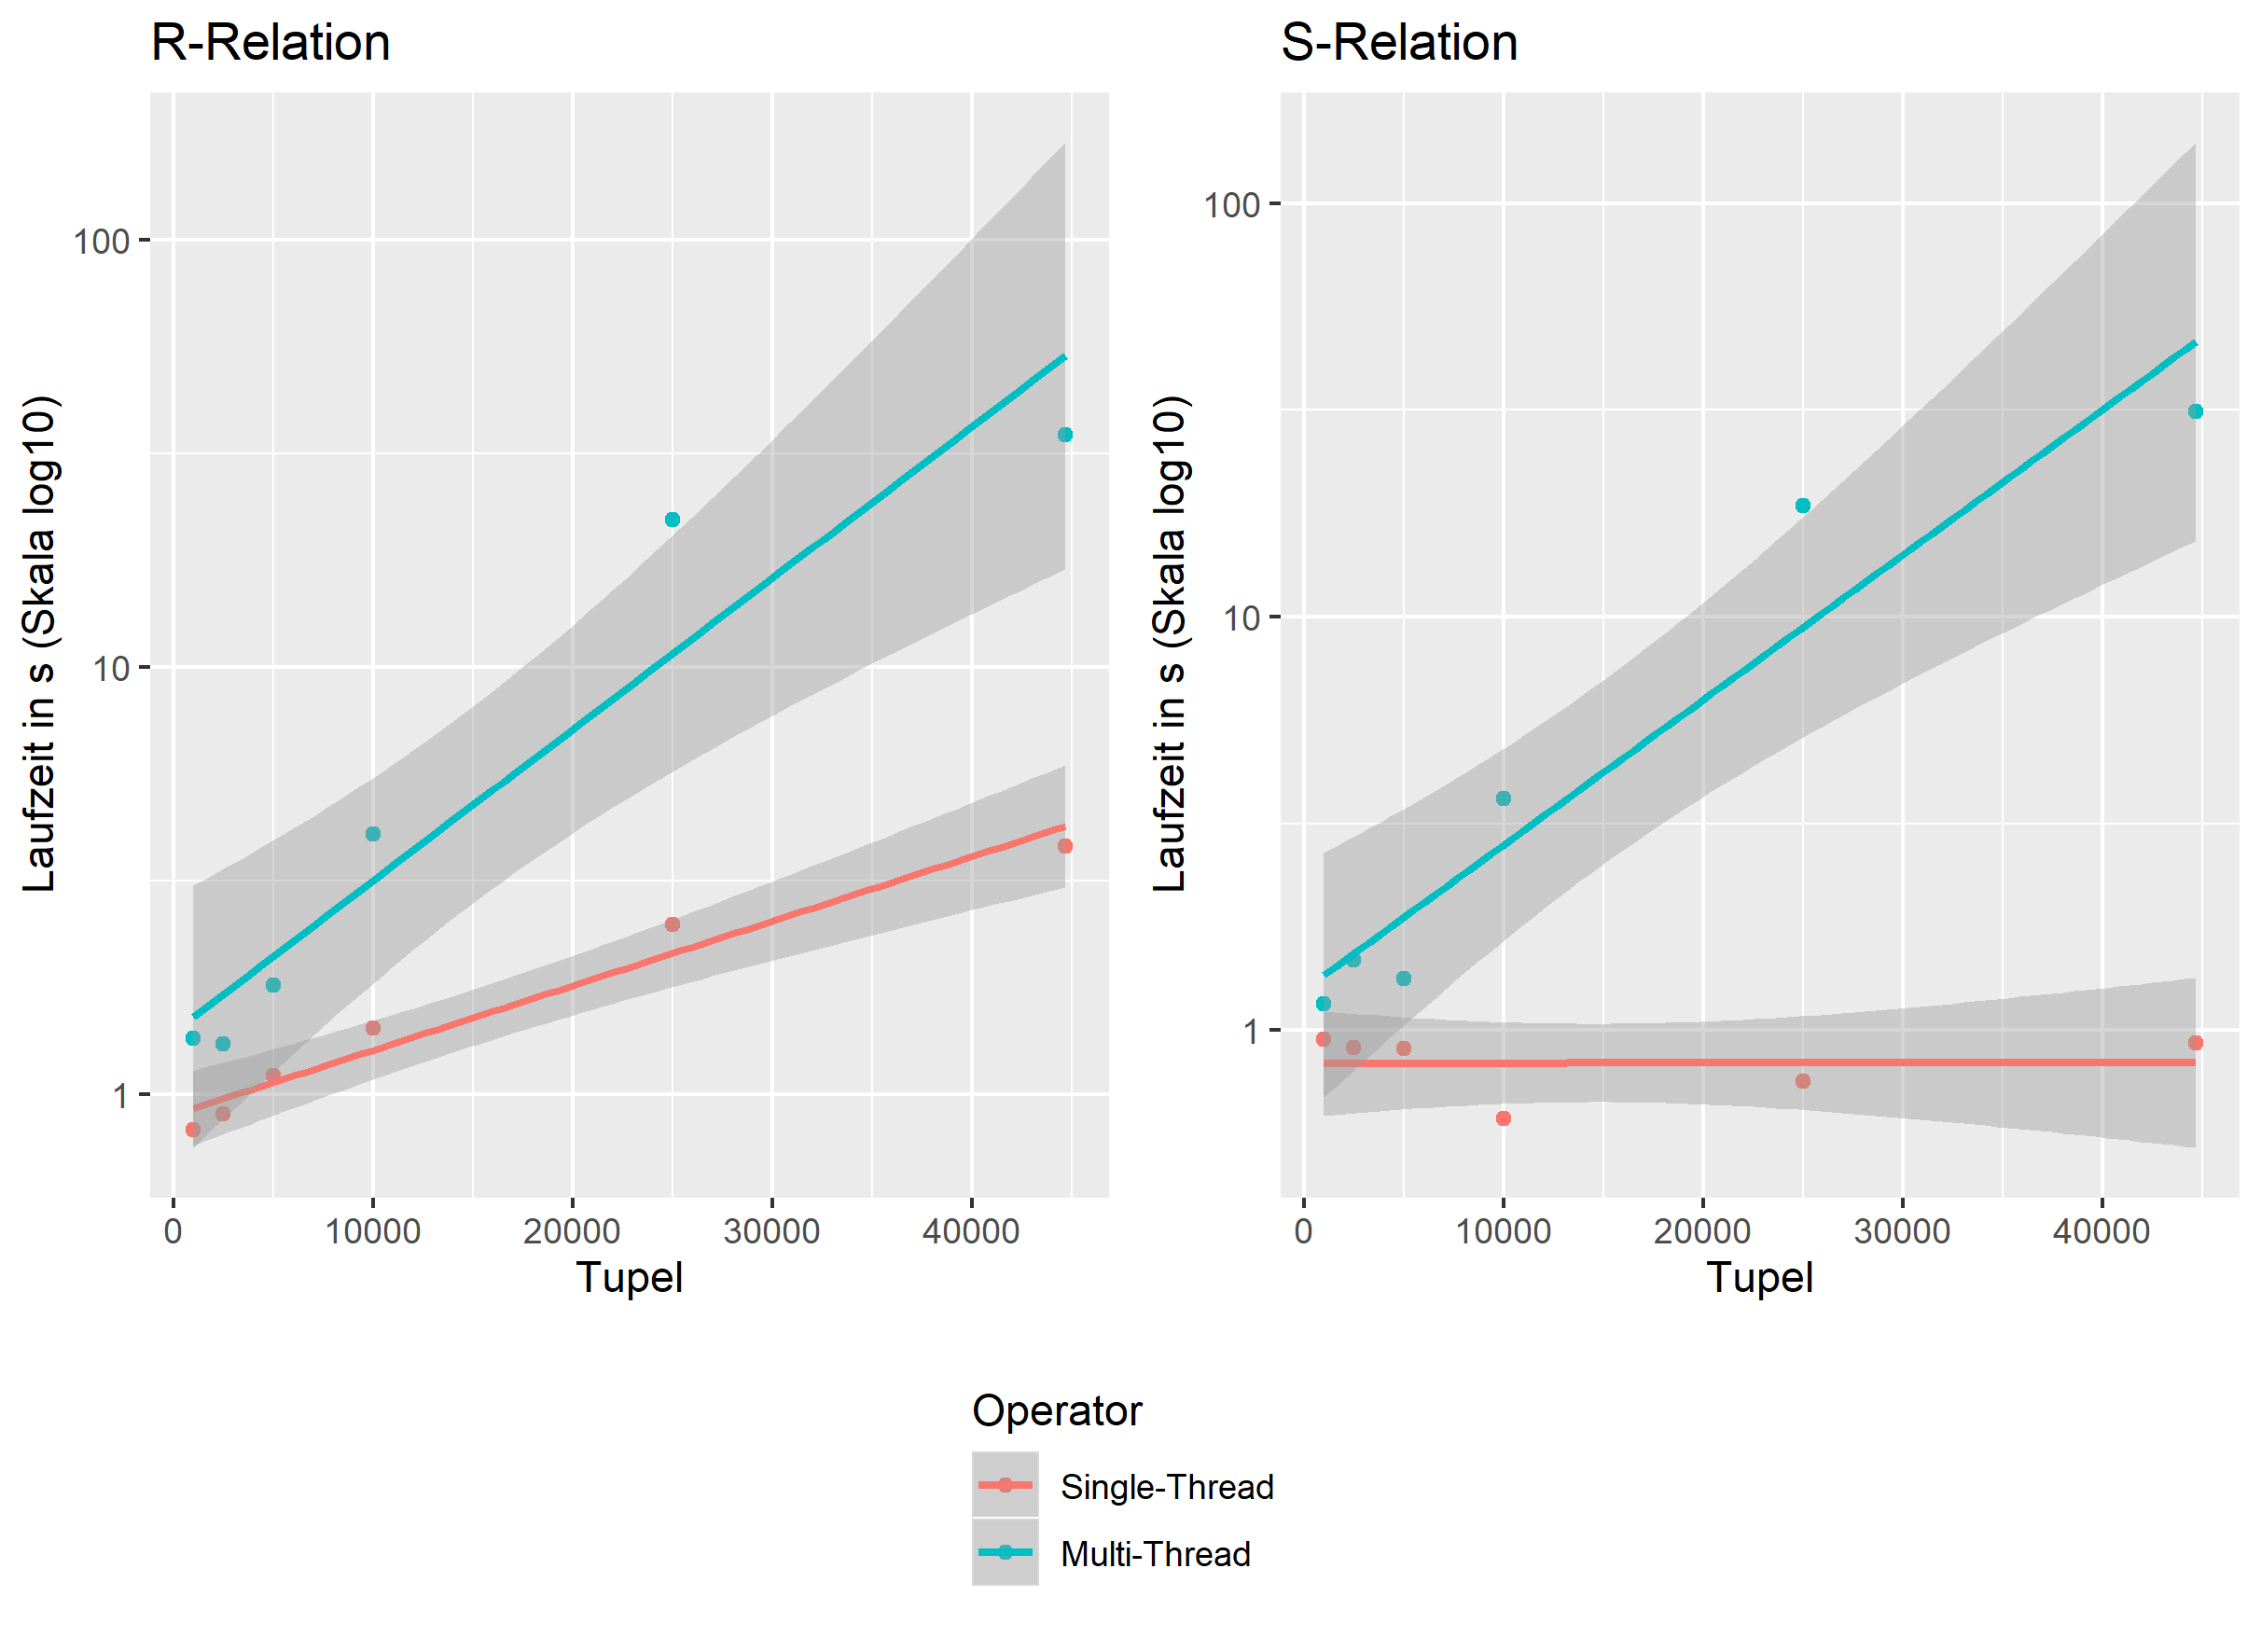
\includegraphics[width=0.45\textwidth]{Bilder/join_head_self2.png}}}
	\caption{Selfjoin \Fb{roads\_str}}
	\label{img:joinExpAllg}
\end{figure}

Im Gegensatz zum Verhalten gegenüber zur dem Speicher, der dem Operator zugewiesen worden ist, zeigt das Verhalten gegenüber der Relationsgröße ein eindeutiges Bild \autoref{img:joinHeadExp}. Große Relationen erhöhen die Laufzeit des von mir implementierten Operators linear. Die lineare Regressionsgerade hat bei wachsender R-Relation für den Multithread-Operator eine stärkere Steigung als die Singlethread-Variante. Interessant ist es vor allem, dass bzgl. einer wachsenden S-Relation sich das Laufzeitverhalten des von mir implementierten Operators in ähnlicher Weise verschlechtert wie bei wachsender S-Relation, aber die Singlethread-Variante hier jenseits von kleinen Schwankungen keine Laufzeitveränderung aufzeigt. Dies deutet an, dass ich ungünstige Entscheidungen für die Implementierung des Hybrid-Hash-Algorithmus getroffen habe. Einige Ideen, wie die Implementierung des Multithreading-Hybrid-Hashs verbessert werden kann, habe ich bereits in \autoref{impl:hybrid} erläutert.   

\begin{figure}
	\centering
	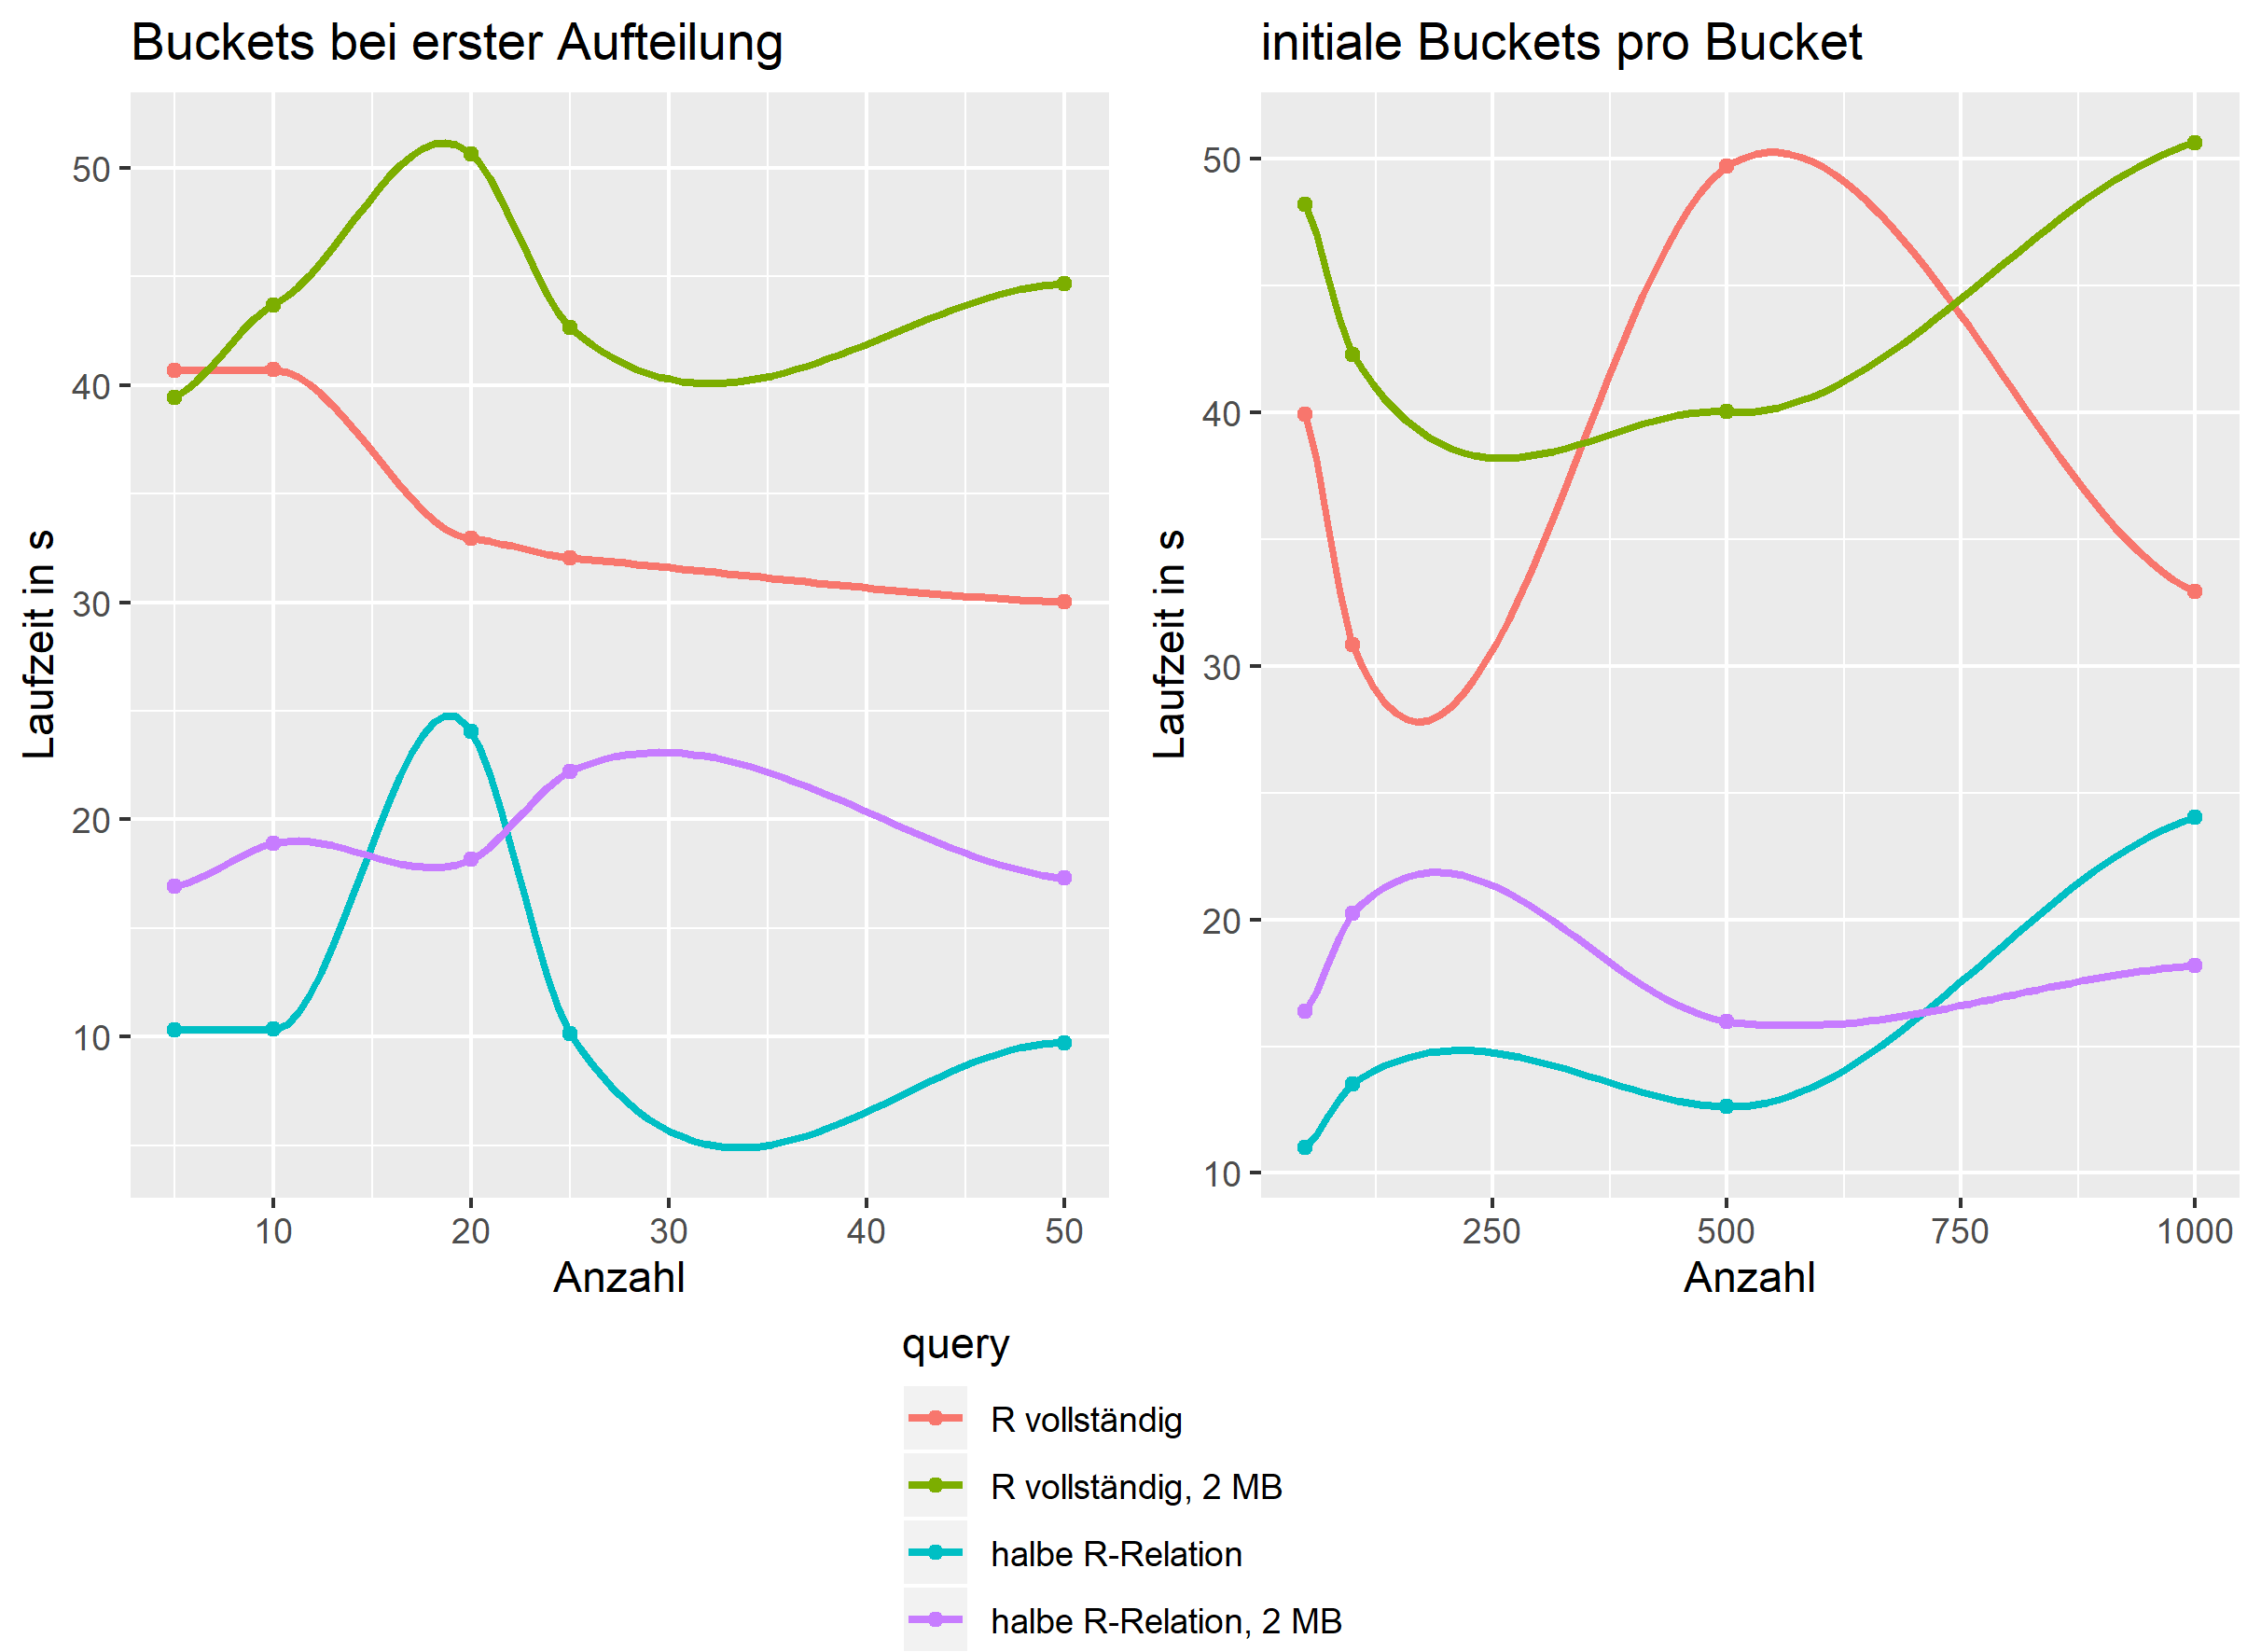
\includegraphics[width=0.70\textwidth]{Bilder/join_bucket.png}
	\caption{Selfjoin der Relation \Fb{roads\_str} nach dem Straßenname bei Veränderung der Anzahl von Buckets.}
	\label{img:joinBucket}
\end{figure}

Der von mir implementierte Hybrid-Hash-Join teilt den Tupelstrom drei Mal in Buckets auf: für die Partitionierung auf die Threads, dann innerhalb jedes Threads auf eine kleine Zahl Buckets, von denen der Erste direkt verarbeitet wird und abschließend jedes Bucket in jedem Thread in so viele Buckets, dass in jedem Bucket sich möglichst nur ein Tupel befindet. Für die letzte Aufteilung wird ein initialer Wert verwendet. \autoref{img:joinBucket} zeigt Glättungskurven für die Veränderung der Laufzeit einerseits nach der Bucketzahl der ersten Aufteilung im Thread und andererseits nach der initialen Bucketzahl, die in jedem Bucket im Thread wiederum angelegt werden (für die erste Aufteilung im Thread wird hier der Standardwert 20 verwendet). Jenseits der Bucketzahl wurde auch die Größe der R-Relation verändert und der zur Verfügung stehnde Speicher reduziert, damit Auslagerungen und rekursive Aufteilung von nicht in den Hauptspeicher passende Buckets vorgenommen werden müssen.

Die erste Aufteilung entscheidet vor allem darüber, inwieweit Buckets ausgelagert werden müssen. Optimal ist ein Wert, bei dem jeder Bucket in den Hauptspeicher passt und gleichzeitig die Anzahl der Buckets möglichst gering ist, da der erste Bucket, der direkt verschnitten wird, möglichst viele Tupel fasst. Negative Auswirkung hat es auch, wenn die Größe so gewählt wird, dass rekursive Ausführung des Hashing-Algorithmus notwendig werden, was vor allem dann auftritt, wenn die Relation bzgl. des Join-Attributs ungleich verteilt ist. Bei einer großen Relation und ohne eine Einschränkung des zur Verfügung stehenden Arbeitsspeichers gibt es dementsprechend einen Schwellwert für die Bucketzahl, an dem die optimale Speichernutzung erreicht ist und dementsprechend sich das Laufzeitverhalten deutlich ändert. Alle anderen Änderungen haben keine große Auswirkung. In allen betrachteten Beispielen gibt es einen oder sehr wenige gewählte Bucketmengen, die sich negativ auf die Laufzeit auswirken.

Die Anzahl initialer Buckets gilt nur für den ersten Bucket in jedem Thread, der direkt verschnitten wird. Trotzdem hat seine Größe eine deutlich Auswirkung auf das Laufzeitverhalten. Sofern viele Tupel in dem gleichen Bucket einsortiert werden, ist ein Verschneiden über eine Schleife notwendig -- der Algorithmus nähert sich also einem Loop-Join an. Dementsprechend die die Auswirkung stärker bei großen Relationen, da mehr Tupel auf eine Hashtabelle verteilt werden. Nach erreichen eines Optimums, bei dem jeder vorkommende Hashwert auf ein eignen Bucket aufgeteilt wird, ist keine Veränderung mehr zu erwarten. Bis zu diesem Punkt verändert sich das Laufzeitverhalten schwankend, da es vorkomen kann, dass auch bei mehr verwendeten Buckets eine Verteilung ungleichmäßiger wird. Im Gegensatz dazu hat der zur Verfügung stehende Arbeitsspeicher für den Operator nur insofern einen Einfluss, dass weniger Tupel auf die Buckets verteilt werden müssen, sich also das Optimum früher einstellt und gleichzeitig die Schwankungen nicht so stark ausgeprägt sind, da im Durchschnitt auch weniger Tupel mit gleichen Hashwerten vorhanden sind.

\subsubsection{Experimente MThreadedSpatialJoin}
\label{exp:sj}

Um das Laufzeitverhalten des Multithreading-Spatial-Joins zu verstehen, habe ich drei unterschiedliche Experimente durchgeführt: Bei verschiedenen Relationen, einem Selfjoin von \Fb{roads} und [$waterways \bowtie roads$, habe ich die Größe der R- und S-Relation variiert (\autoref{img:sjExpHeadAllg}). Bei einem einer Verschneidung der Relationen \Fb{roads} und \Fb{landuse} habe ich dem Operator unterschiedlich viel Arbeitsspeicher zur Verfügung gestell \autoref{im:sjMemExp} und bei dem gleichen Join die Konfiguration des Verwendeten R-Baums bei unterschiedlich großen Relationen variiert \autoref{img:sjTreeExp}.

\begin{figure}
	\centering
	\subfloat[Selfjoin\label{img:sjHeadExpRr}]{{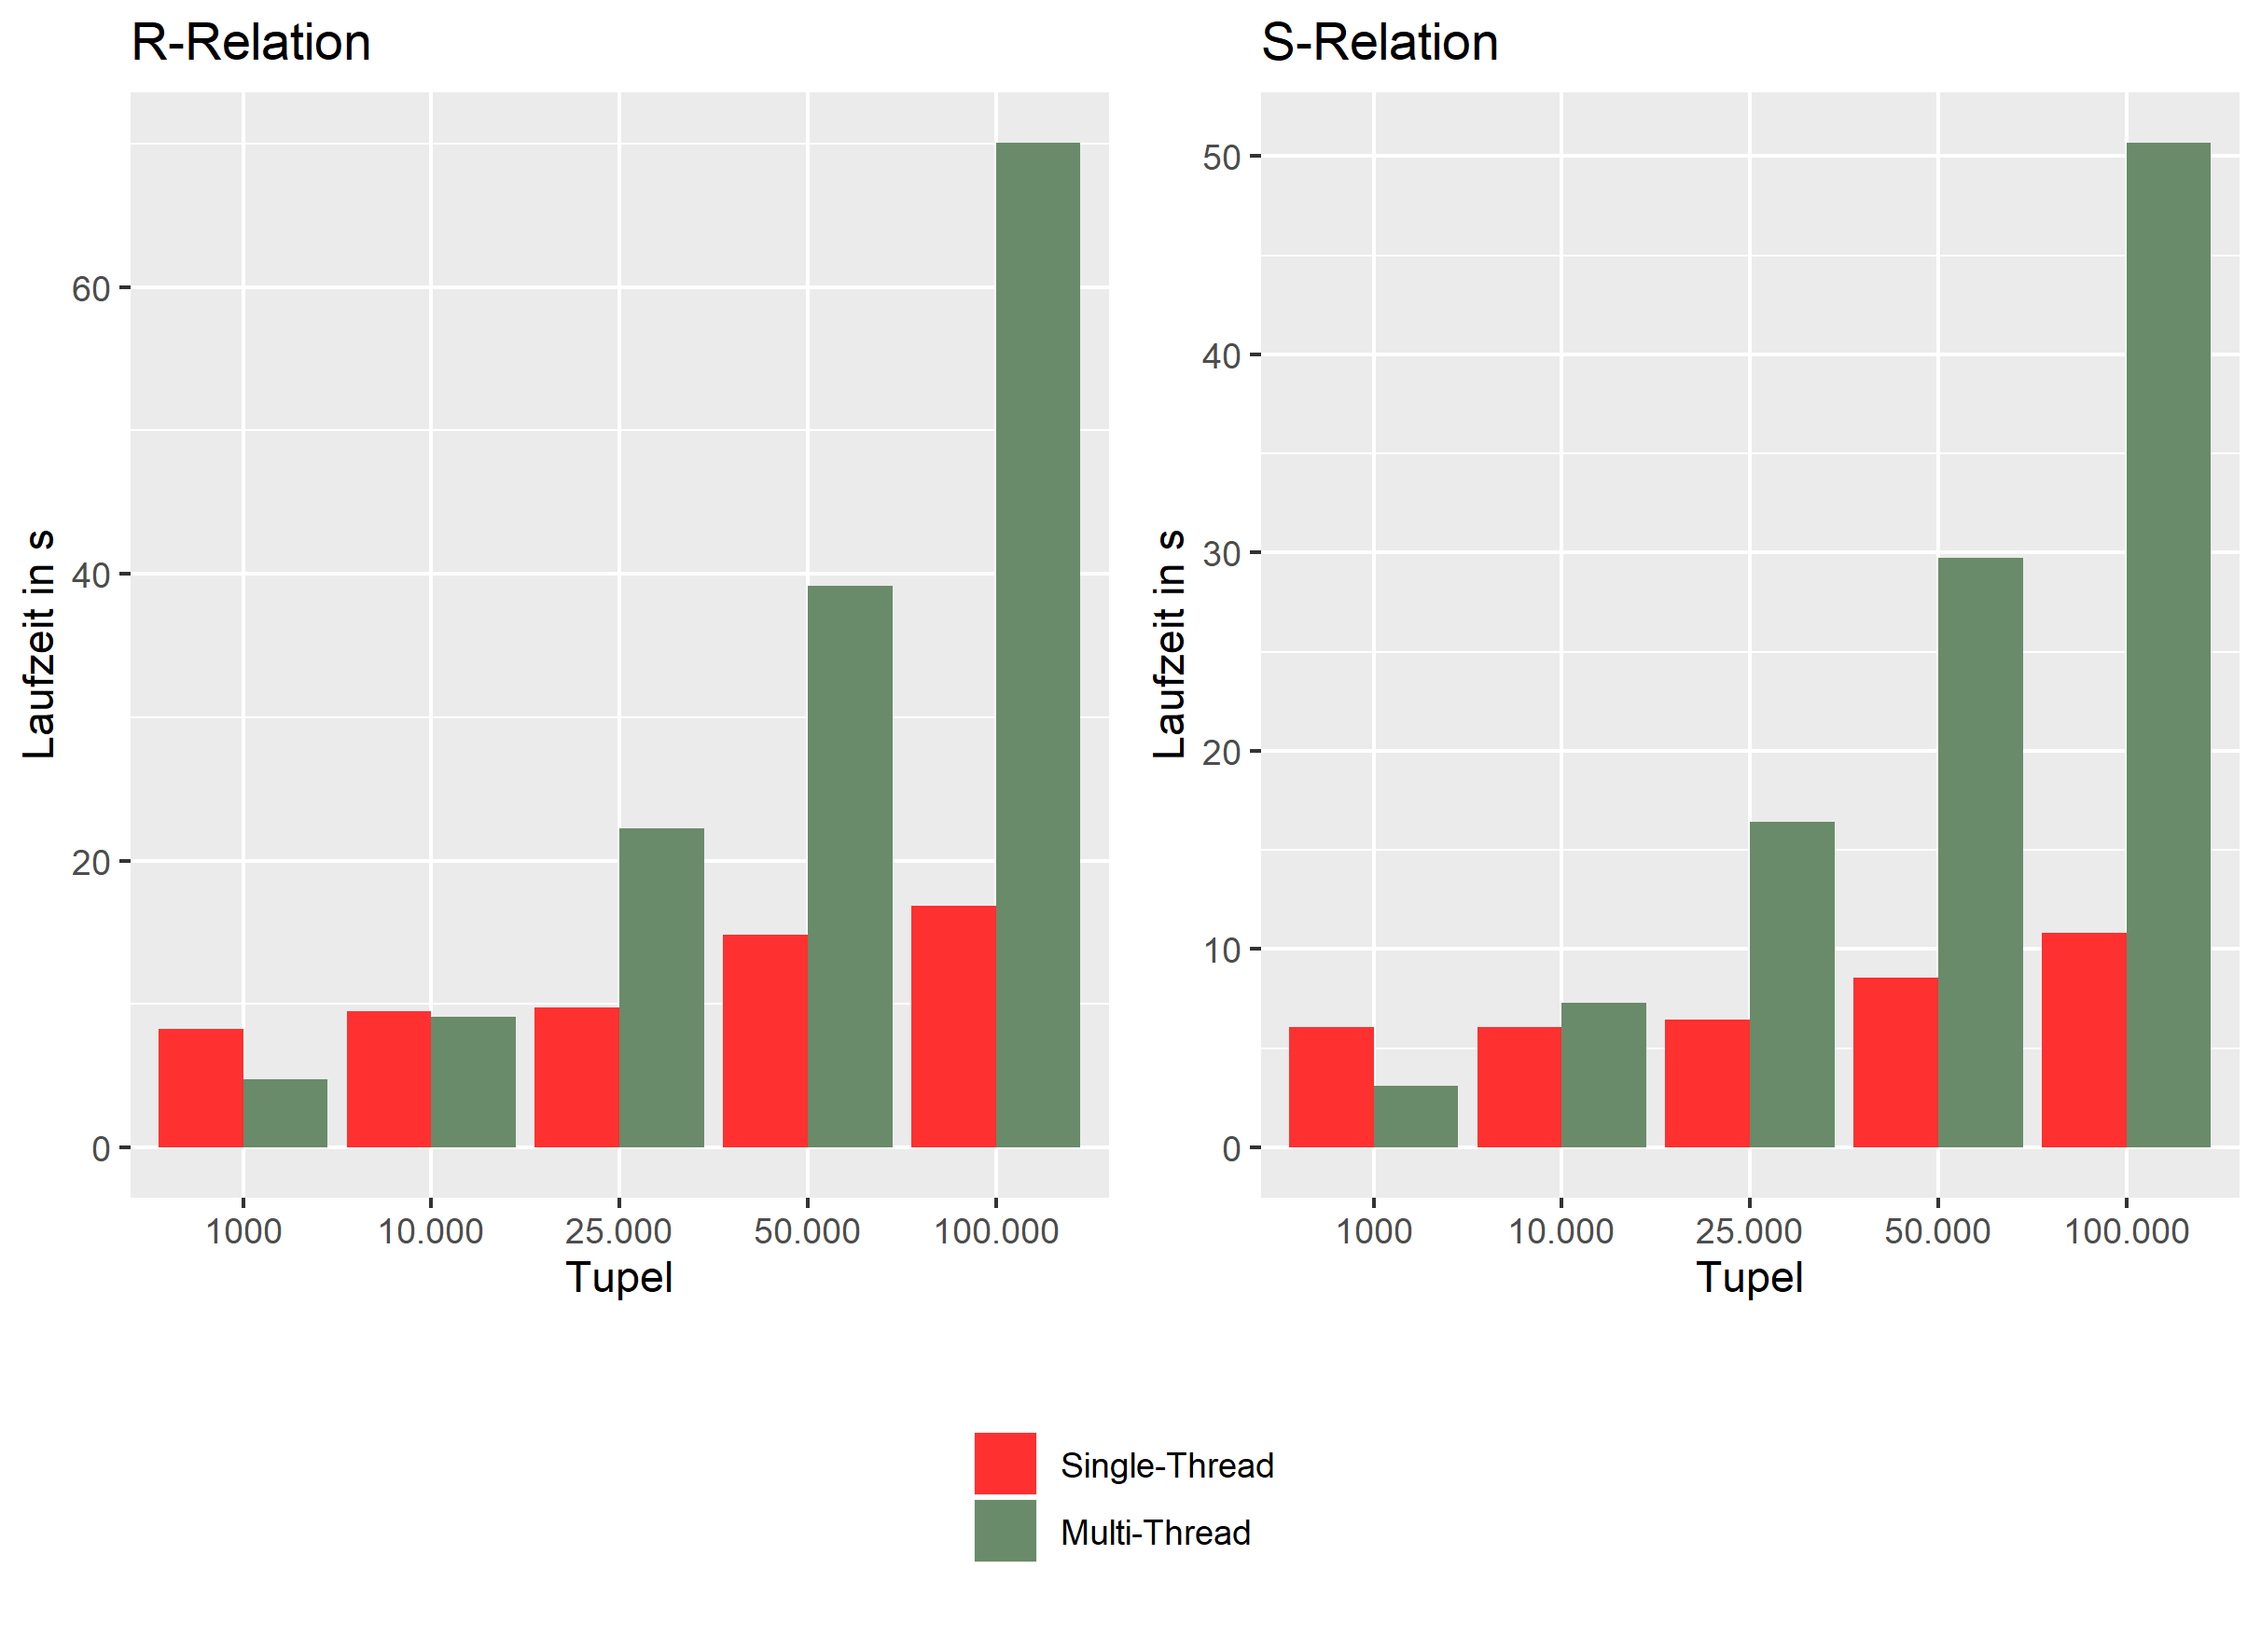
\includegraphics[width=0.60\textwidth]{Bilder/sj_head_rr.png}}}
	\qquad	
	\subfloat[$waterways \bowtie roads$ bzw. $roads \bowtie waterways$\label{img:sjHeadExpWr}]{{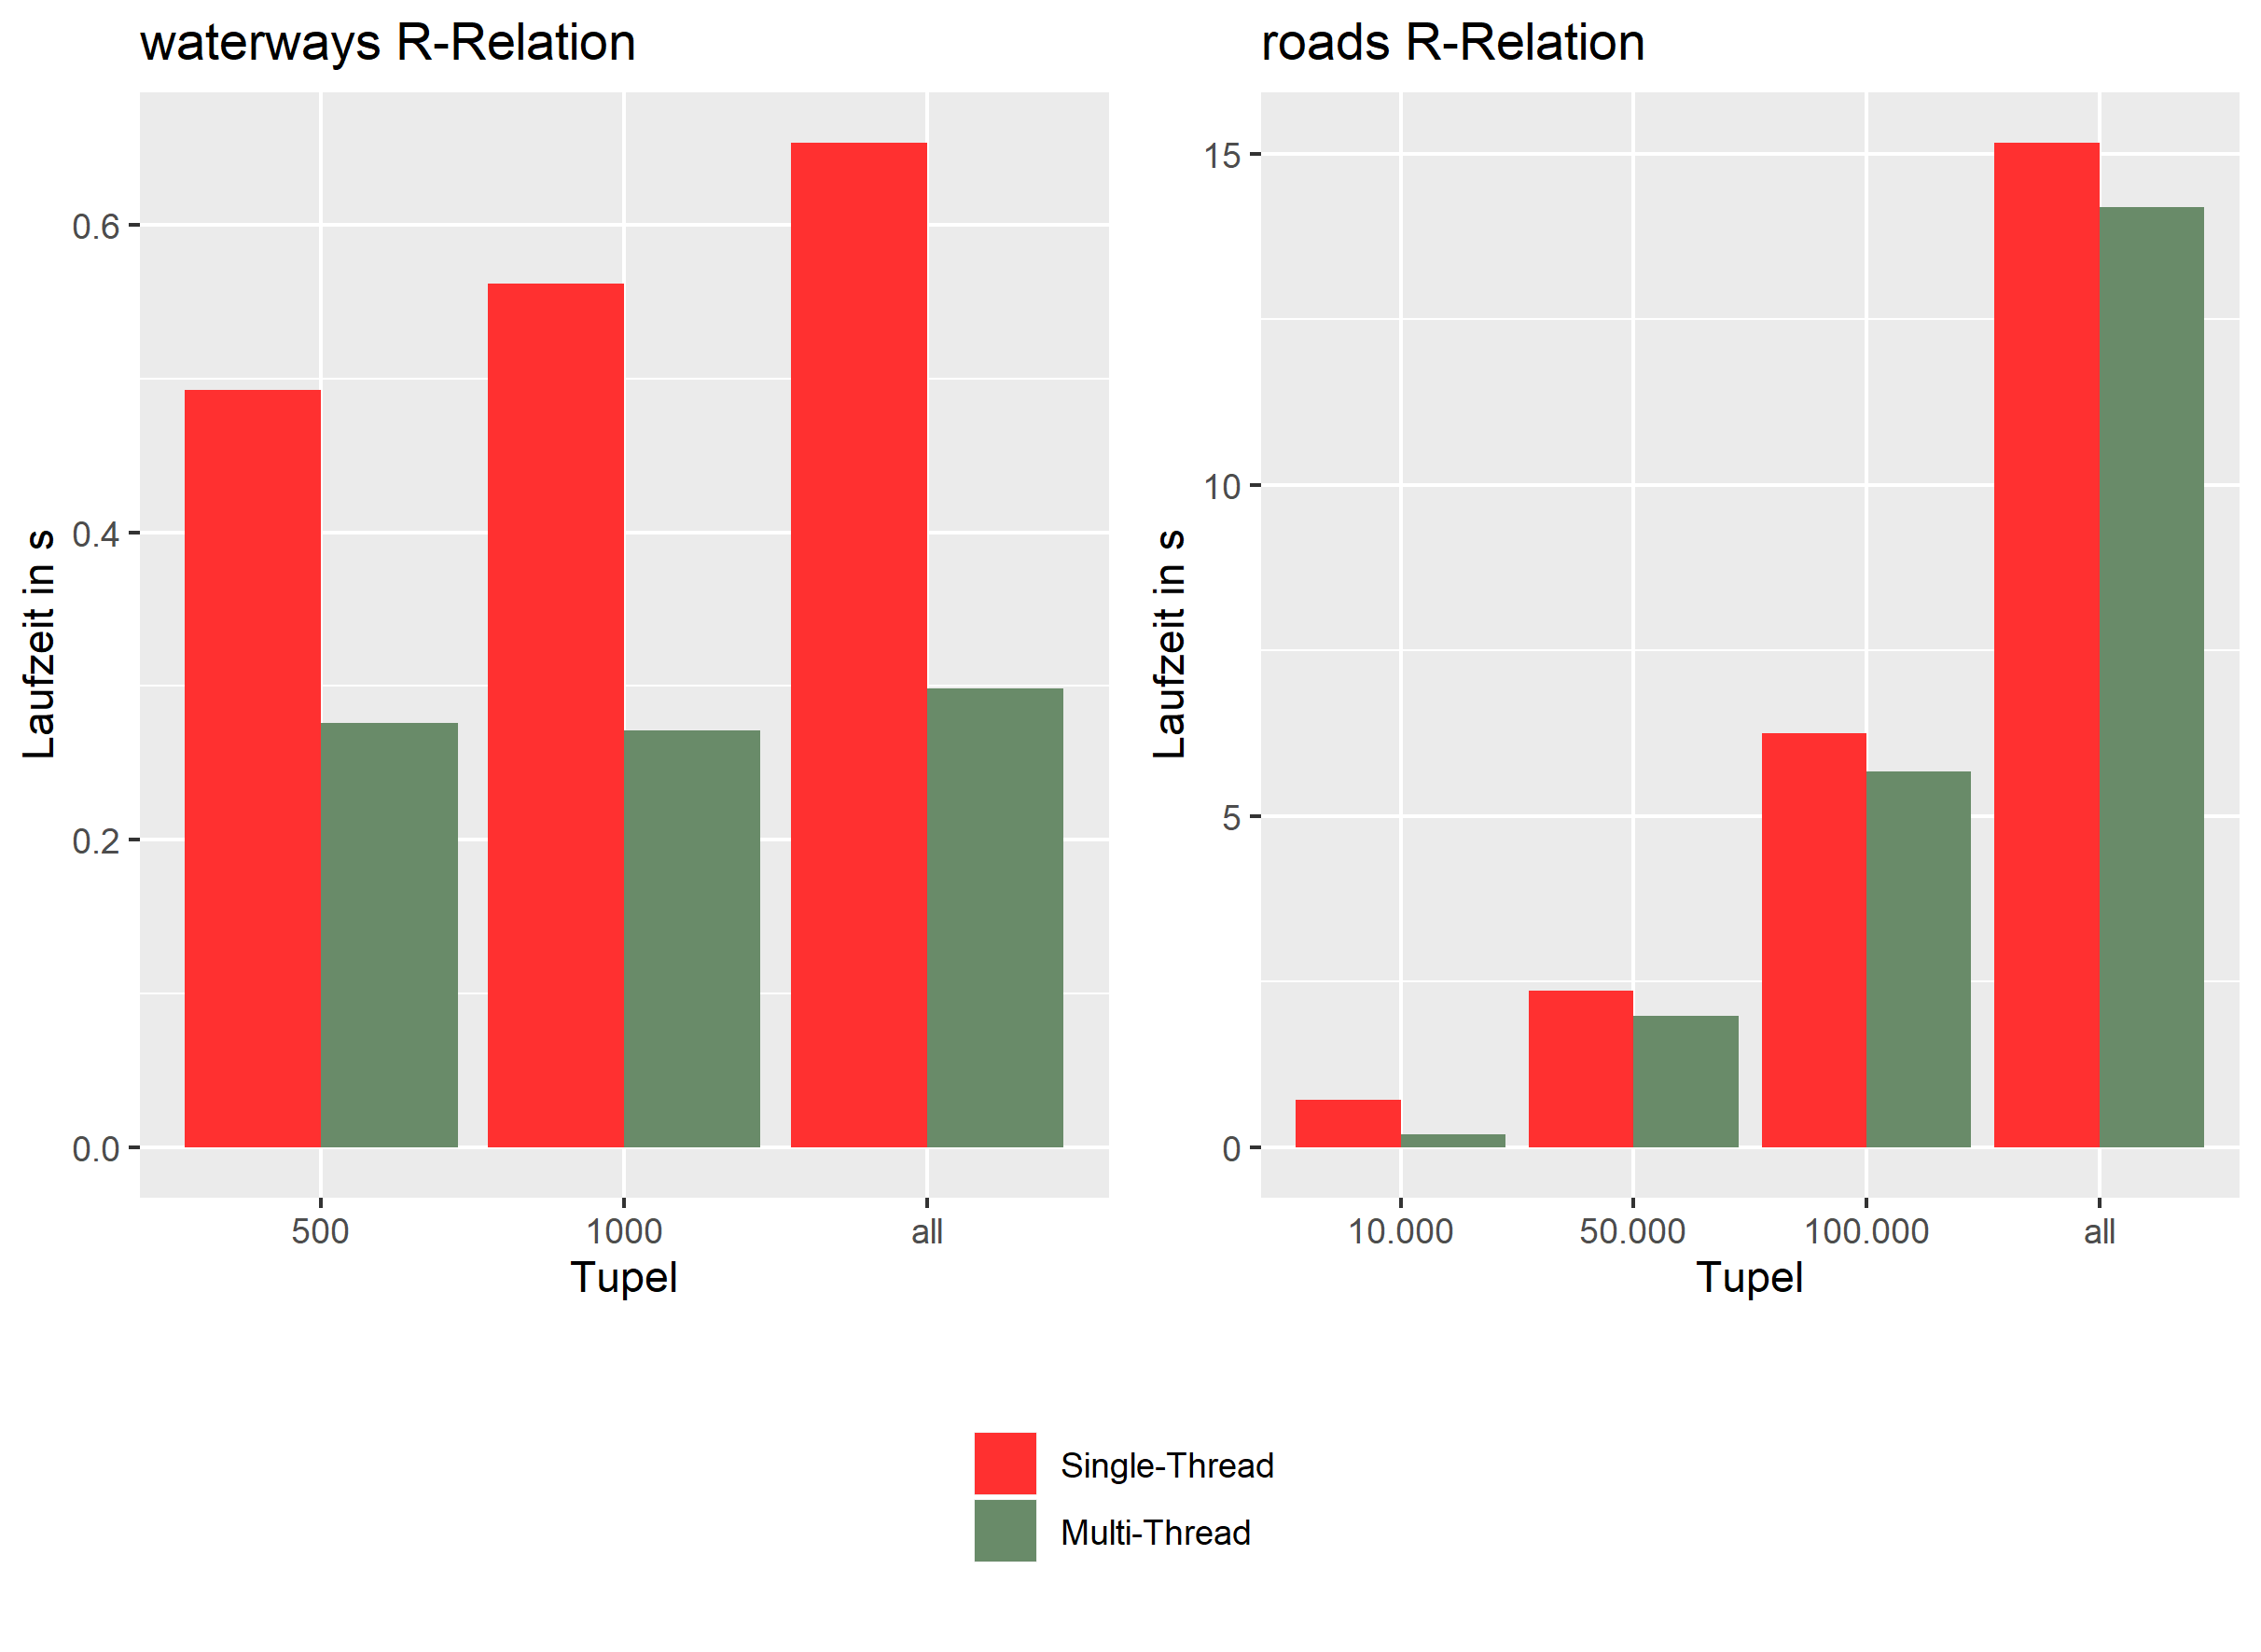
\includegraphics[width=0.60\textwidth]{Bilder/sj_head_wr.png}}}	
	\caption{Spatial Joins mit unterschiedlichen Relationen und Relationsgrößen}
	\label{img:sjExpHeadAllg}
\end{figure}

Effizienter ist der von mir implementierte Algorithmus lediglich bei kleinen Relationen, sowohl bzgl. der R- als auch der S-Relation. Bei dem Selfjoin, dessen Laufzeitanalyse in \autoref{img:sjHeadExpRr} dargestellt ist, ist der Anstieg der Laufzeit bei der Singlethread-Variante nahezu linear, bei der Multithread-Variante exponentiell. Also ist wahrscheinlich eine ungünstiger Algorithmus der Grund, dass die Performancevorteile bei kleinen Relationen bei deren Vergräßerung verloren gehen. Im Experiment, dessen Ergebnis in \autoref{img:sjHeadExpW} dargestellt ist, wurden die R- sowie die S-Relation ausgetauscht und dann die Größe der R-Relation variiert. Die eine Relation, die die Wasserwege in Berlin darstellt, ist sehr klein (2104 Tupel). In beiden Fällen ist der Anstieg der Laufzeit im Gegensatz zu großen Relationen noch vergleichbar mit der Singlethread-Variante und insgesamt ist die Laufzeit unter Nutzung mehrerer Kerne besser. 

\begin{figure}
	\centering
	\subfloat[nach verfügbarem Speicherplatz\label{img:sjMemExp}]{{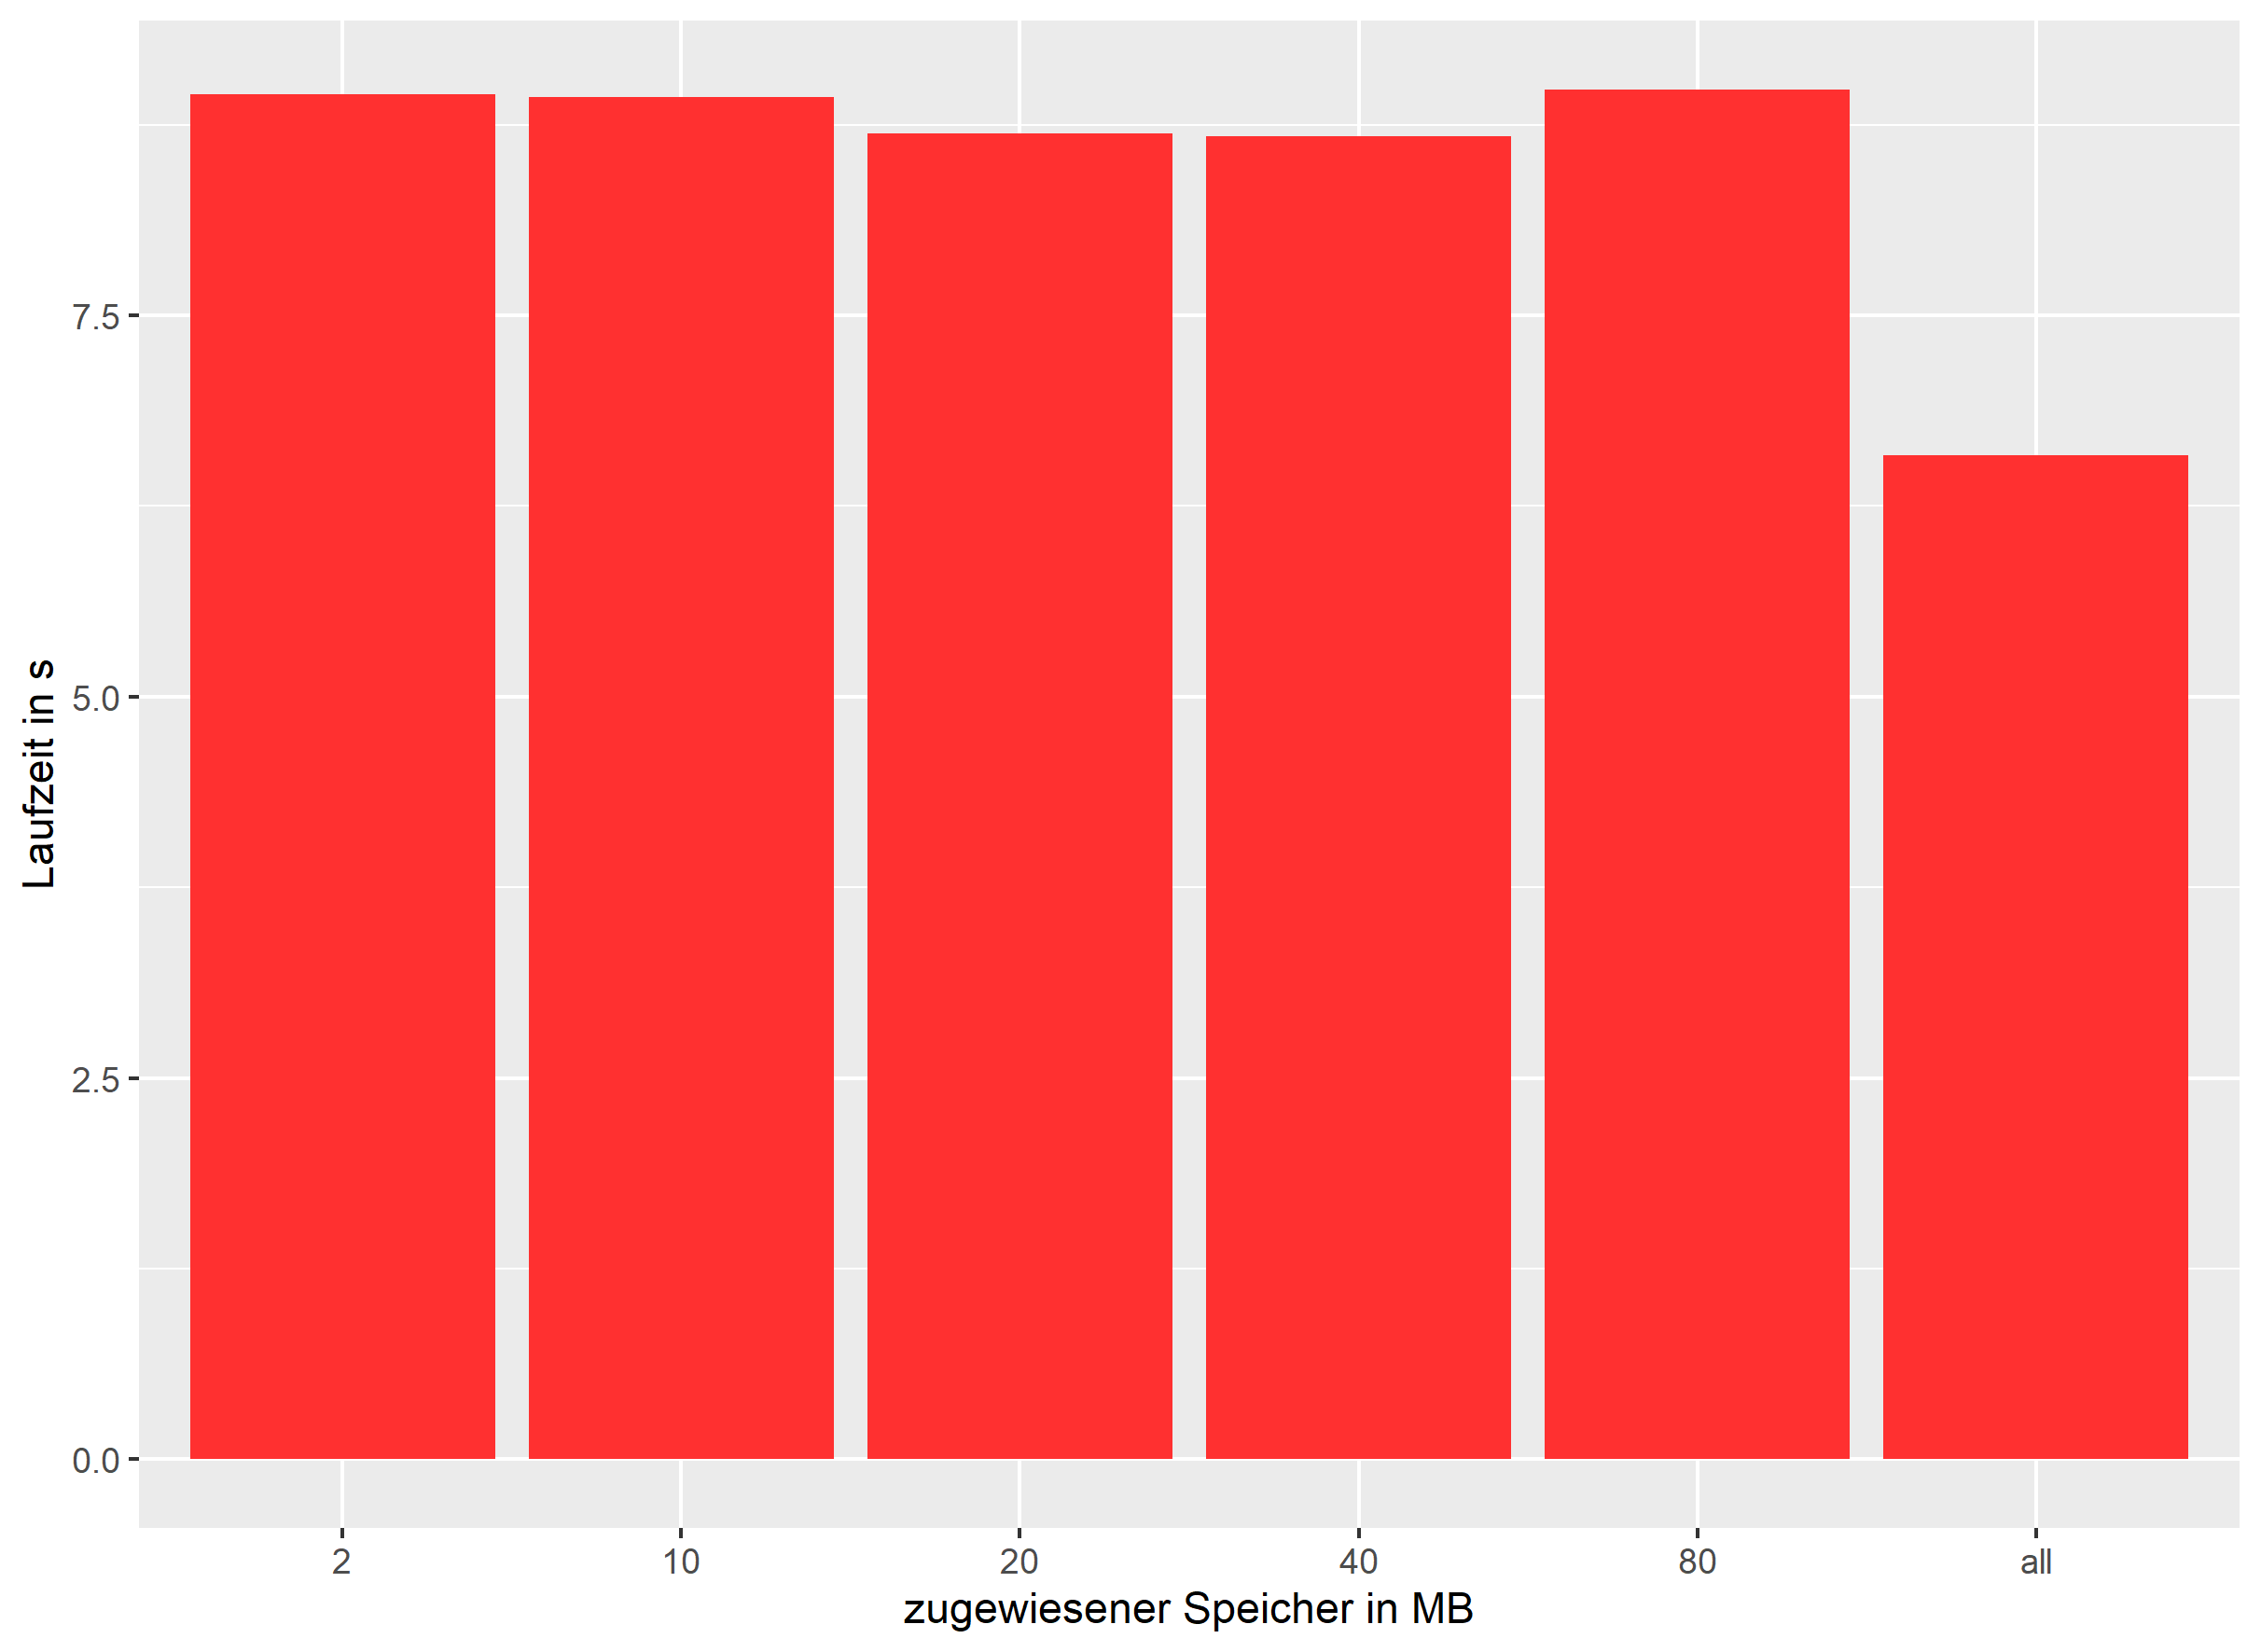
\includegraphics[width=0.45\textwidth]{Bilder/sj_mem.png}}}
	\subfloat[Konfiguration des R-Baums\label{img:sjTreeExp}]{{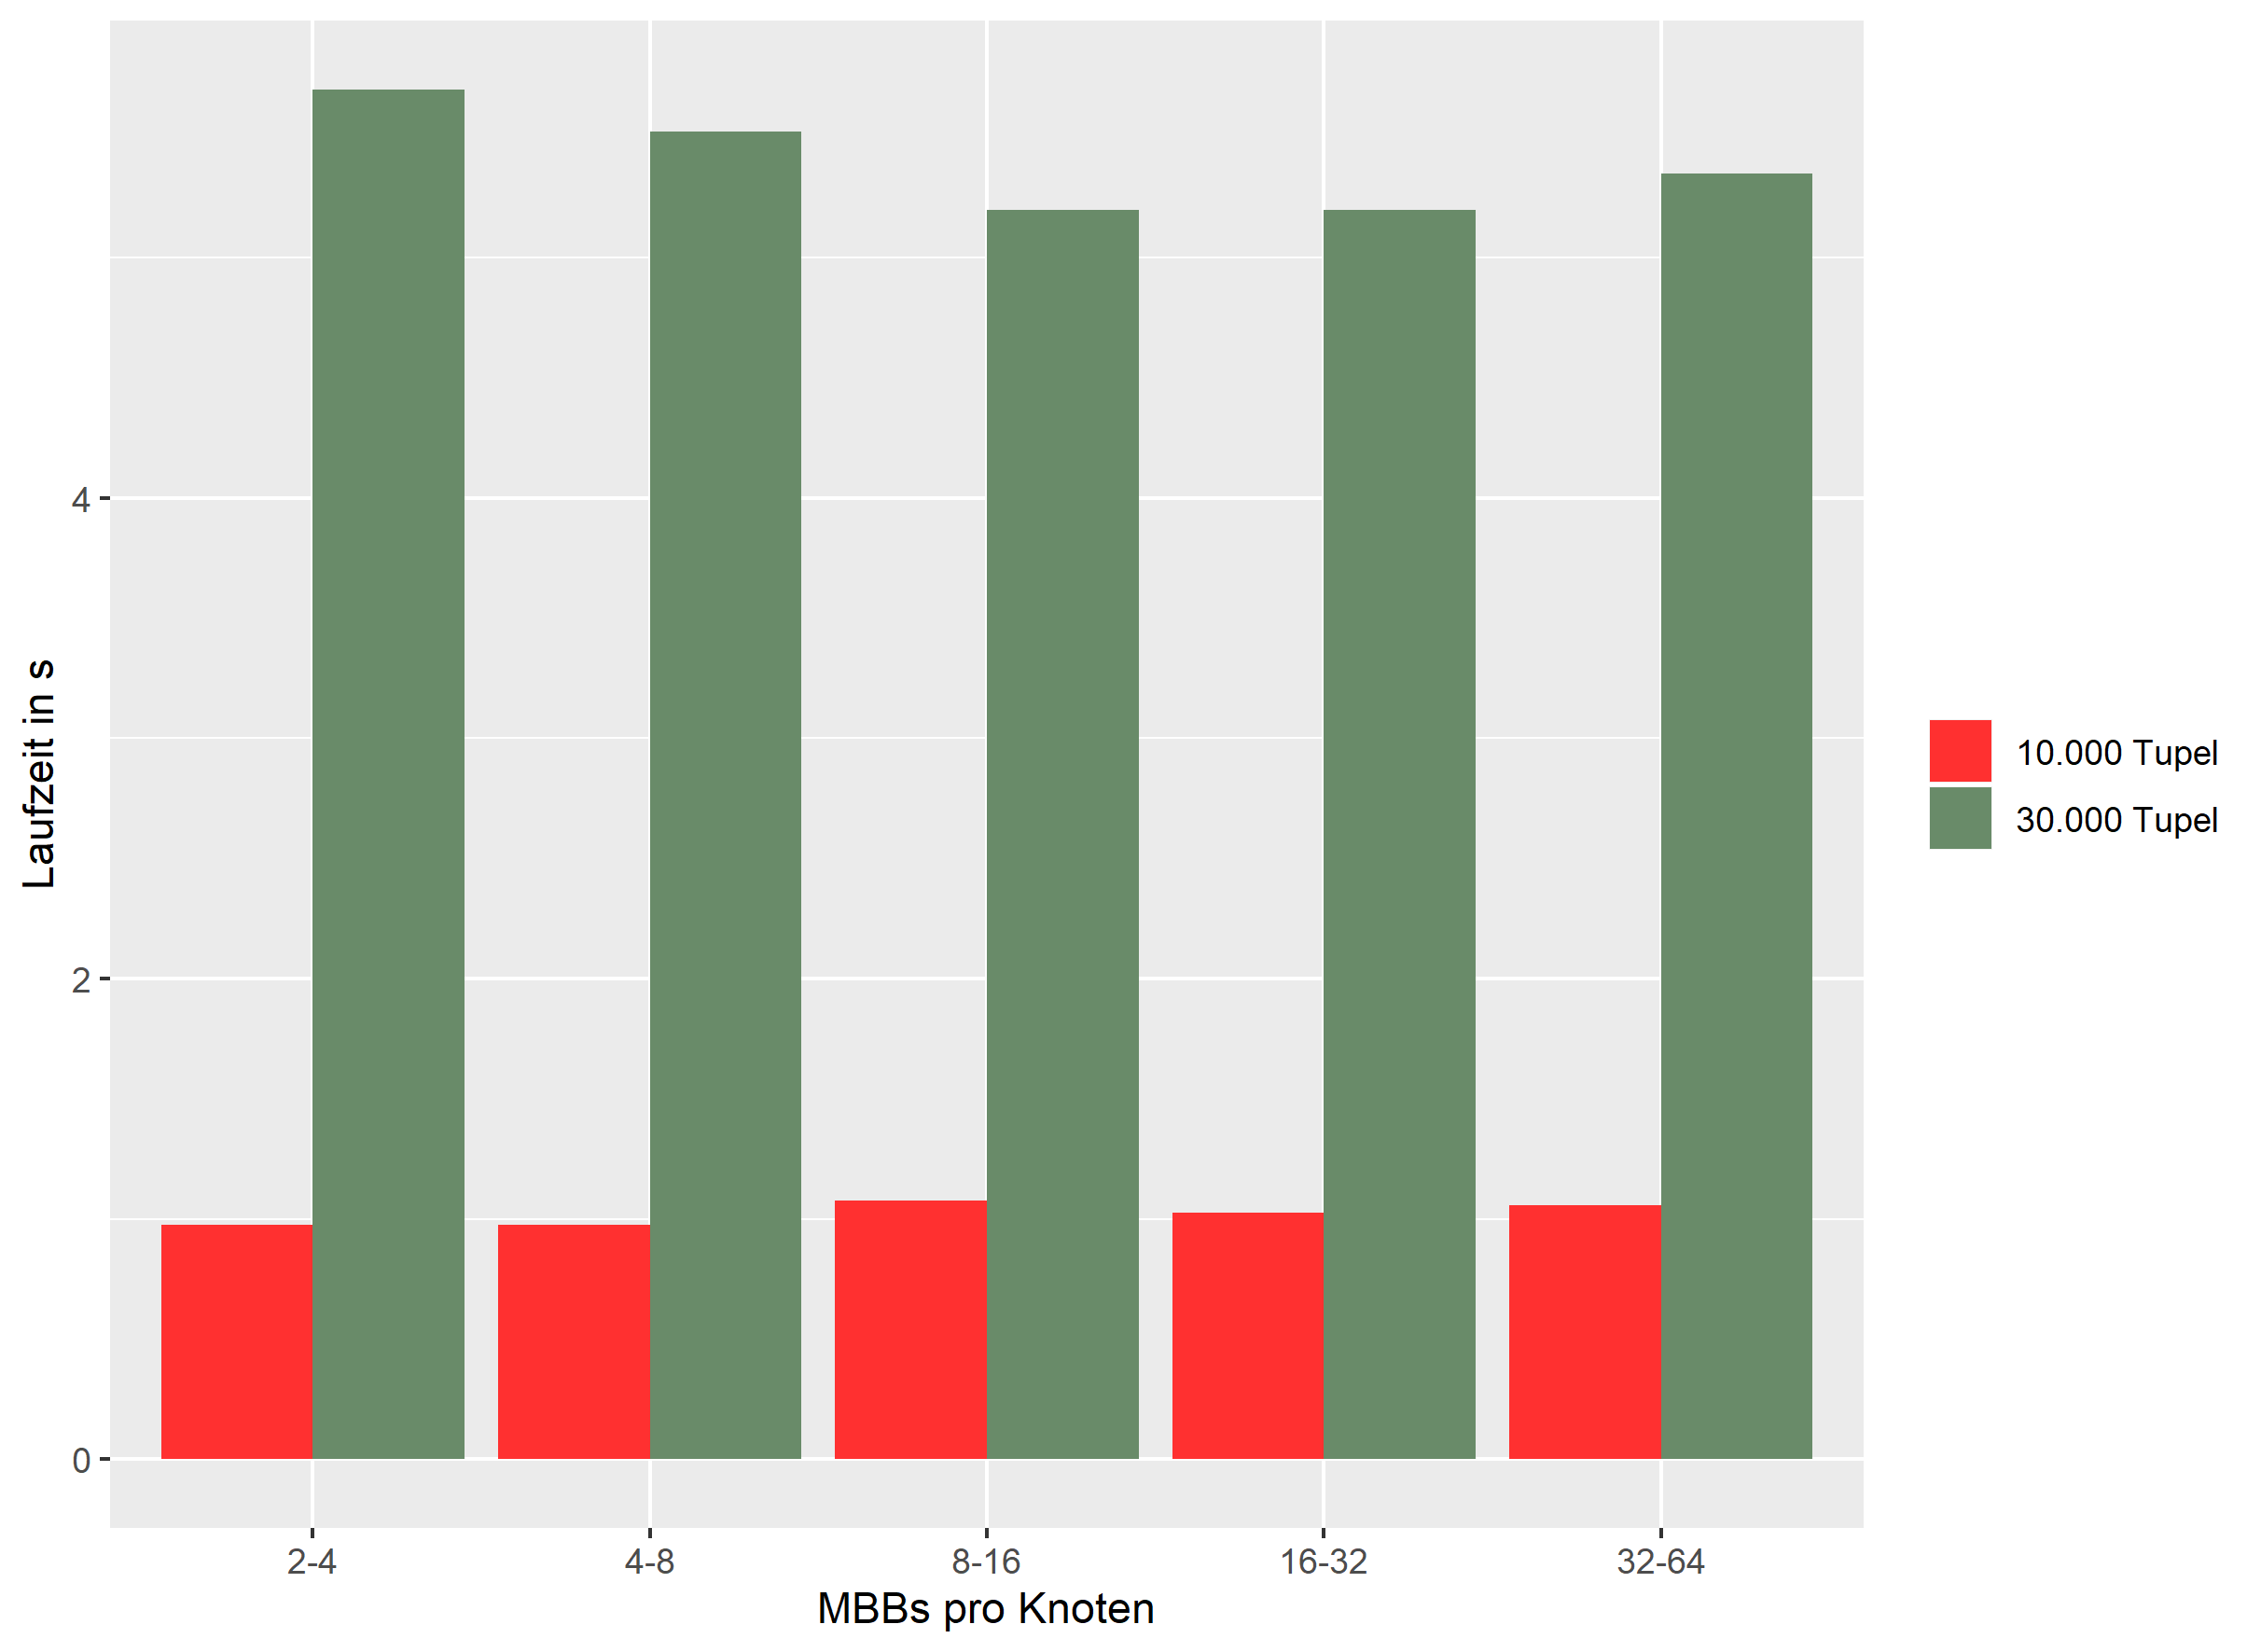
\includegraphics[width=0.45\textwidth]{Bilder/sj_tree.png}}}
	\caption{Verschiedene Experimente mit dem Spatial Join}
	\label{img:sjExpAllg}
\end{figure}

\autoref{img:sjMemExp} zeigt die Veränderung der Laufzeit, wenn der dem Operator zur Verfügung stehende Speicher reduziert wird. Hier gibt es nur eine Spring von 80~MB zum Speicher, dem der Operator im Standardfall zur Verfügung steht. Der Operator benötigt mehrere Iterationen und muss Teile der R-Relation auslagern, wenn für die vollständige interne Struktur (also für die Tupel der R-Relation und den R-Baum) für diese Relation nicht genügend Speicher zur Verfügung steht. Hier ist das Verhalten des Operators merkwürdig, da bereits ab 80~MB keine Auslagerungsdateien mehr notwendig sind und bei 40~MB für jeden Thread nur eine Iteration notwendig ist, bei weniger Speicher mehr. Die I/O-Operationen sind also für den Operator nicht geschwindigkeitsbestimmend. Dies steht im Gegensatz dazu, dass zu Beginn vermutet wurde, dass gerade die I/O-Operationen in einer Systemarchitektur mit geteiltem Permanentspeicher Dateioperationen das Nadelöhr sind, da hier kein paralleler Zugriff möglich ist. Dementsprechend muss bei dem Multithrad-Spatial-Join die Bedeutung der CPU-Zeit für die Laufzeit deutlich dominieren.

Auch eine Konfiguration des R-Baums hat nur sehr wenig Auswirkung auf die Laufzeit. Für den In-Memory-R-Baum habe ich $2-4, 4-8, \ldots, 32-64$ Einträge pro Knoten gewählt. \autoref{img:sjTreeExp} zeigt, dass die Veränderung der Zahl der Einträge und damit der Höhe des Baums nur eine sehr geringe Auswirkung hat auf das Laufzeitverhalten. Wahrscheinlich wäre dies bei deutlich größeren Relationen anders, aber bei 10.000 bzw. 30.000 Tupel lohnt es nicht, den R-Baum beispielsweise über die Attribute des \Fb{mThreadedSpatialJoin}s parametrisierbar zu machen.   

\subsubsection{Experimente MThreadedFilter}
\label{entw:filter}

Eigentlich habe ich bei dem Filteroperator einen großen Performancegewinn erwartet, sofern die Prädikate einen hohen Rechenaufwand bedürften, was bei Operationen mit komplexen räumlichen Typen der Fall ist. Allerdings zeigt der Operator ein eindeutig schlechteres Laufzeitverhalten als die Singlethread-Variante und sein Laufzeit nimmt mit der Anzahl genutzter Kerne sogar ab. Interessant ist die Analyse dieses Operators vor allem, da sein eigentlicher Algorithmus sehr simpel ist und ich ungünstige Entscheidungen bei der Implementierung des Filters ausschließen kann. Der Algorithmus beruht vor allem auf der Auswertung eines Prädikats mithilfe von je einem Queryprozessor pro Thread.
  
\begin{figure}
	\centering
	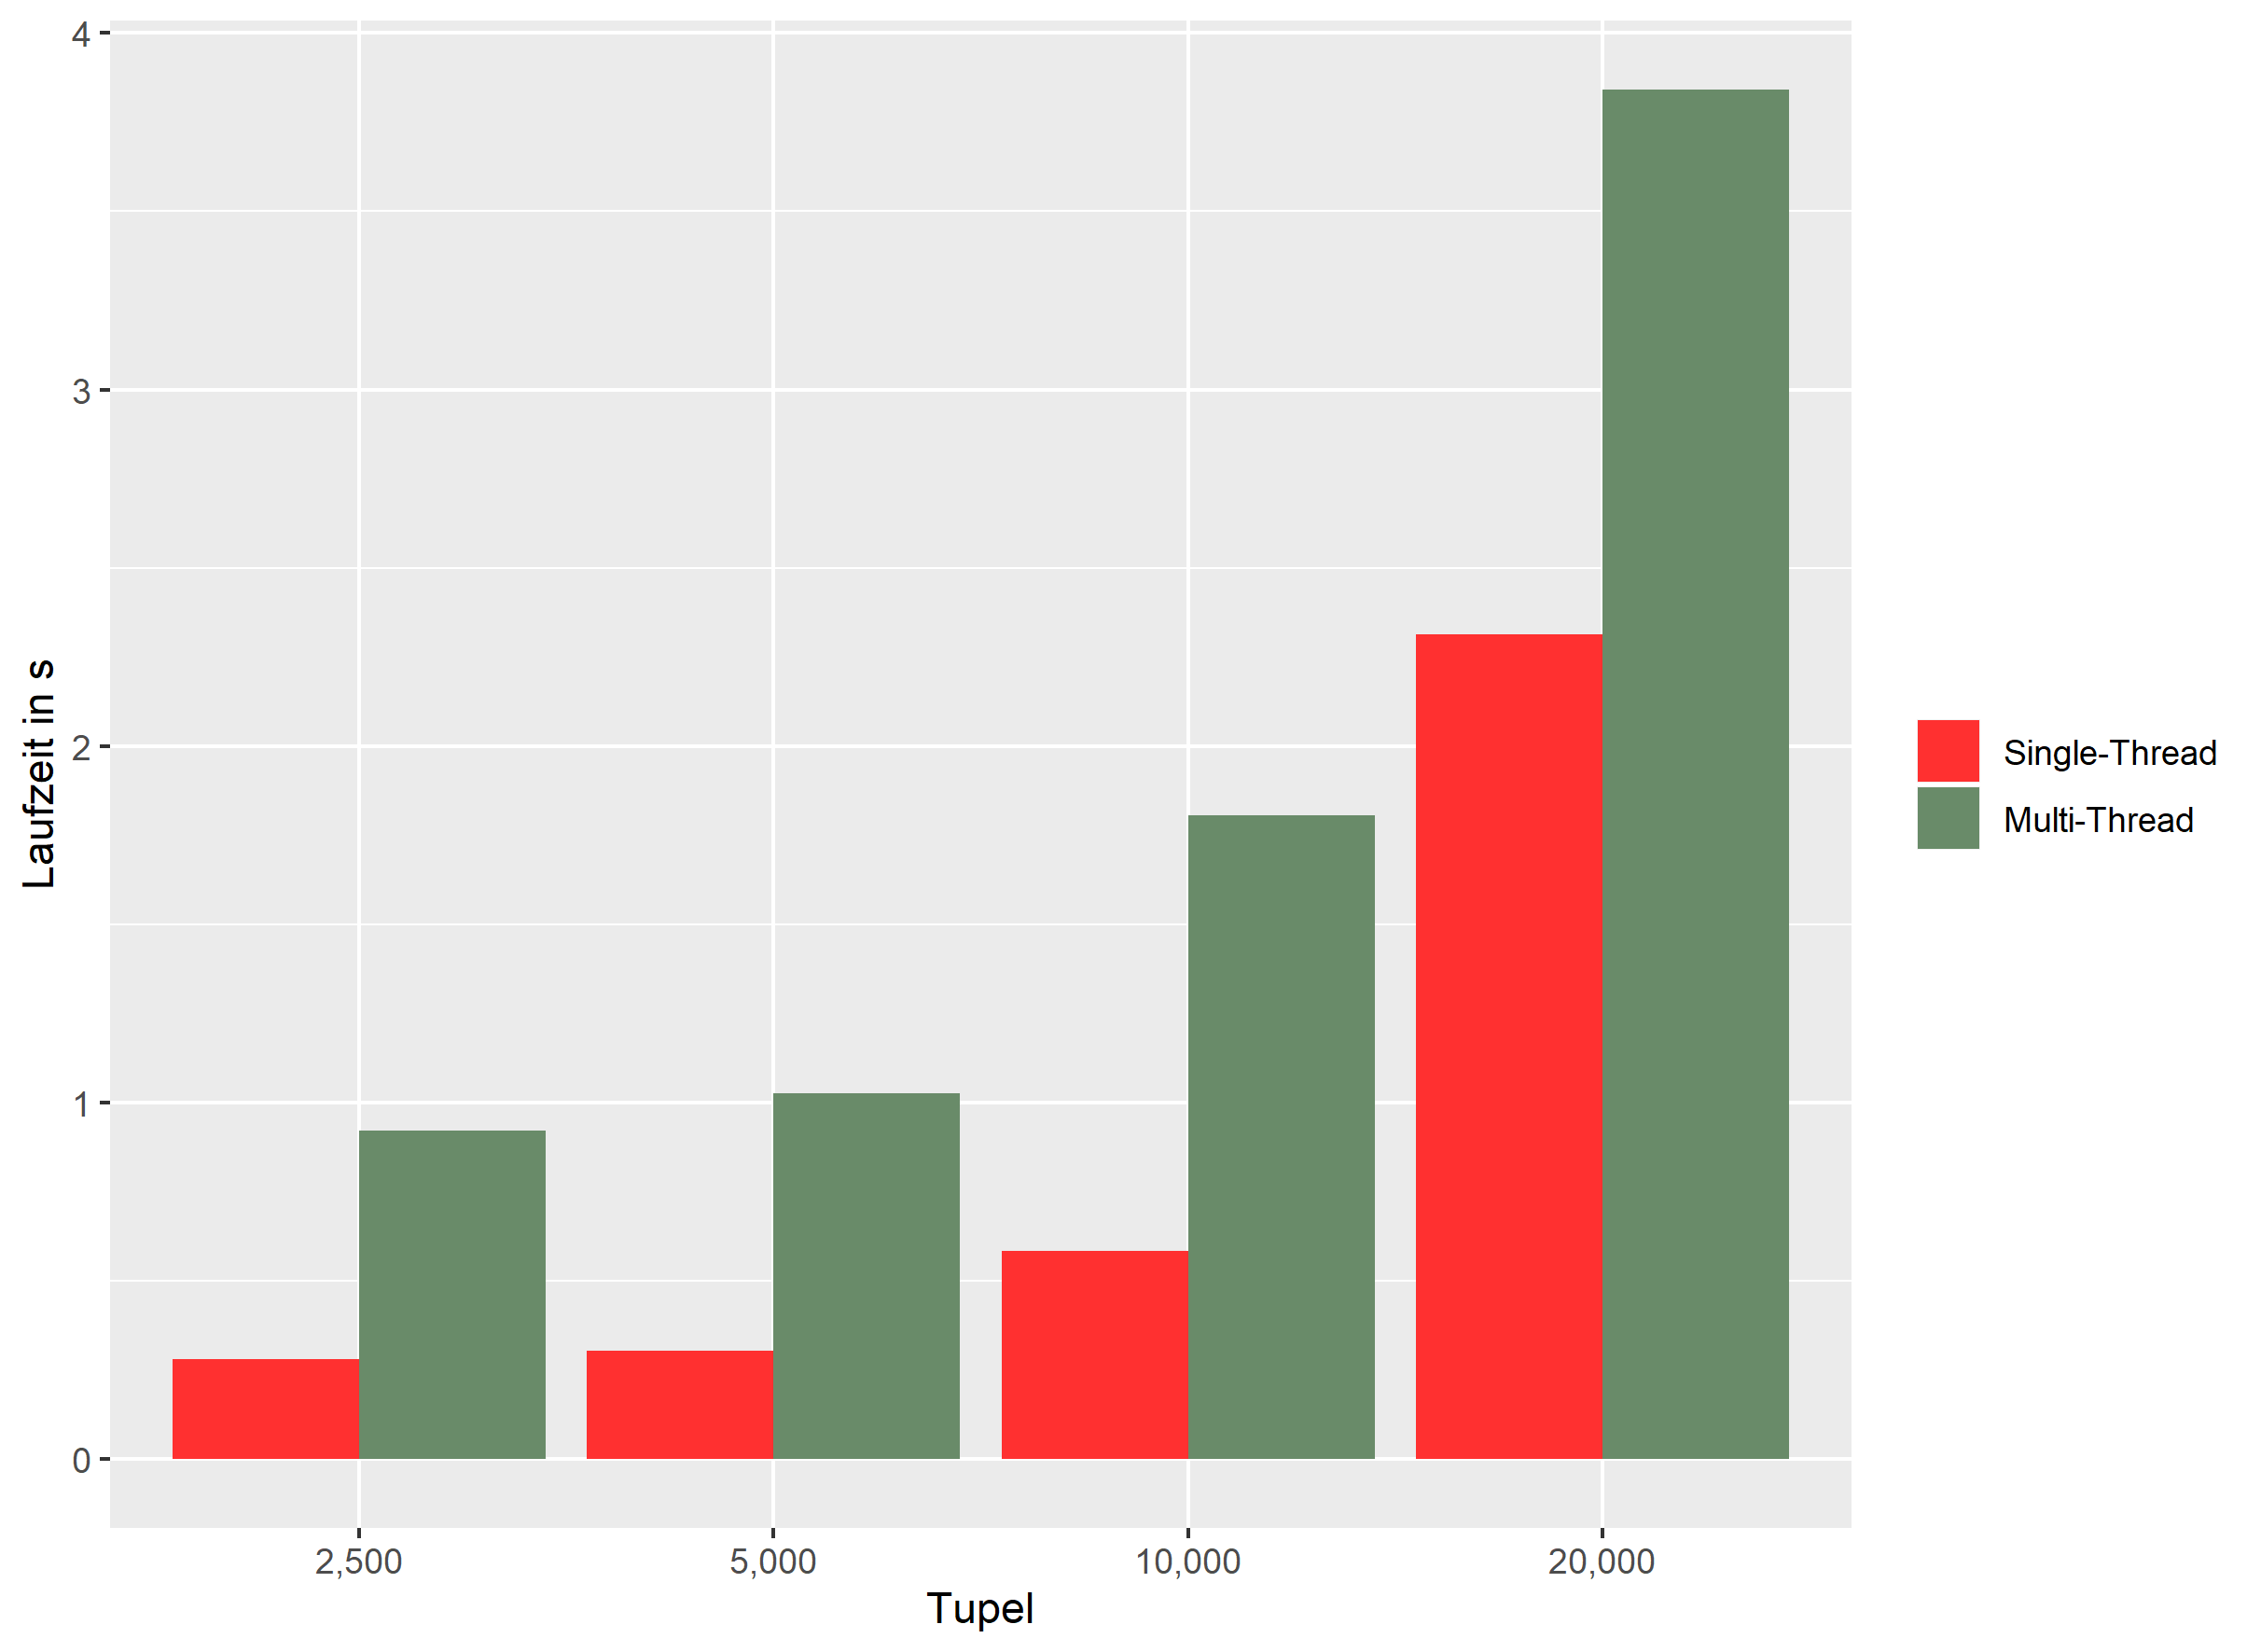
\includegraphics[width=0.70\textwidth]{Bilder/filter_head.png}
	\caption{Filter und verschiedene Relationsgrößen}
	\label{img:filterHead}
\end{figure}

Da der Operator seinen Speicher nicht selbst verwaltet -- dementsprechend macht eine Analyse des Verhältnisses von Laufzeitverhalten und zur Verfügung stehenden Speichers keinen Sinn. \autoref{img:filterHead} zeigt, dass der auf einem Kern ausgeführte Filter-Operator durchgehend schneller ist als die Multithread-Variante. Ausgewertet wurde ein komplexes Prädikat, welches auf Schnittpunkte zweier Linien prüft. Allerdings ist hier der Anstieg der Laufzeit beim Singlethread-Operator schneller. Da diese Entwicklung erst bei der letzten Messung sichtbar ist, ist jedoch eine sichere Vorhersage das Verhalten bei sehr großen Relationen nicht möglich. Eine Überprüfung ist auch nicht möglich, da der Operator wegen des Problems bei der Synchronisierung der Zugriffe auf die Berkeley-DB bei Relationen über 20.000 Tupeln nicht mehr stabil arbeitet. 

Da das Laufzeitverhalten deutlich hinter den Erwartungen zurückbleibt und eine ungünstige Implementierung der Auswertung der Prädikate ausgeschlossen werden kann, muss der Grund für die schlechte Performance entweder im Scheduling liegen oder in der Synchronisierung. Da in der \Fb{Getnext}-Methode der Tupelstrom an alle Worker-Threads verteilt werden muss und gleichzeitig die Ergebnisse aus den Workern weitergereicht werden müssen, ist das Scheduling komlexer als bei einem seriell arbeitenden Filter und erfordert darüber hinaus eine Synchronisierung. Auch benötigen die Warteschlangen, die für den Austausch von Tupeln zwischen dem Hauptthread und den Workern genutzt werden, eine Synchronisierung über Locks. Eine weitere Erklärung für die schlechte Performance der Multithread-Operatoren sind die Synchronisierungen im Secondo-Kern, vor allem beim Zugriff auf \Fb{FLOBs}, die bei den Auswertungen der Prädikate stattfinden (und bei anderen Operatoren auch beim Auslagern von Daten). Eine gute Performance lässt sich also wahrscheinlich nur erreichen, wenn das Scheduling optimiert wird und vor allem versucht wird, die Operatoren so anzulegen, dass teure Synchronisierungen nur selten eingesetzt werden müssen. Auch wenn hier noch einige Optimierungen möglich sind, zum Beispiel mit der Verwendung von je einer eigenen Ergebniswarteschlange für jeden Thread, aus der alternierend ausgelesen wird, ist wahrscheinlich ein wirklich performantes Multithreading-Secondo nur möglich, wenn parallele Zugriffe auf die Speicherschicht des Datenbanksystems zugelassen werden, auch da eine weitere Synchronisierung der \Fb{FLOBs}, die bisher nicht stabil nutzbar sind bei Zugriffen aus mehreren Threads, noch zu weiteren Perfomanceeinbussen durch umfangreiche Locks oder sogar die teuren Bedingungsvariablen führen würde. 

\section{Schlussbemerkungen}

Eine Bewertung der Implementierung einer Algebra für Multithread-Versionen ausgewählter Operatoren erfolgt anhand der in \autoref{problem} gesetzten Ziele. Eine Implementierung je einer parallelen Version der Operatoren Sort, Equi-Join und Spatial-Join erfolgte inkl. der zwei Schritte des Spatial-Joins, des Filter- und des Refinement-Schritts, die alle mit mehr als 3 Threads lauffähig sind, teils auch mit deutlich mehr Threads als dem System zur Verfügung stehen. Alle Operatoren haben mindestens den gleichen Funktionsumfang wie die Singlethread-Versionen. Beim Spatial-Join-Operator ist es darüber hinaus noch möglich, die Minimal Bounding Box zu vergrößern, so dass sich dieser auch als Filter-Schritt für räumliche Verschmelzungen eignet, deren Prädikate einen Abstand der im Prädikat verwendeten räumlichen Objekte voraussetzen, wie zum Beispiel Joins nach Nachbarschaften. Unter fast allen Bedingungen liefern die Operatoren richtige Ergebnisse. Die einzige Ausnahme ist hier der Hash-Join, der Tupelpaare ignoriert, wenn ein Joinattribut so häufig mit einem gleichen Hashwert vorkommt, dass das entsprechende Bucket nicht mehr in den Hauptspeicher passt. Hier wäre ein Abbruch des Operators sinnvoller, da in diesem Fall ein Hash-Join ein sehr schlechtes Laufzeitverhalten hat und dementsprechend nicht mehr sinnvoll ist.

Die zweite und sehr deutliche Einschränkung der Robustheit ist ein grundsätzliches Problem des Secondo-Kerns in der Synchronisation der Zugriffe auf die Berkeley-DB bzw. die bisherige Einschränkung, dass auf der Storage-Manager keine parallelen Zugriffe auf die Berkeley-DB zulässt. Vor allem sofern \Fb{FLOBs} verwendet werden, reicht die bisherige Synchronisierung von Secondo nicht aus, die vor allem im Flob-Manager stattfindet, so dass abhängig davon, wie häufig die \Fb{FLOBs} in den Hauptspeicher geladen werden müssen, Fehler entstehen, die zu Abstürzen oder Deadlocks führen. Hier wurde versucht, die Synchronisation des Secondo-Kerns zu verbessern, allerdings ohne Erfolg. Auch wenn von mir die Probleme des Kerns für ein paralleles Secondo nur eingegrenzt, aber nicht vollständig identifiziert worden sind, werden folgende Schritte wahrscheinlich notwendig sein, um sinnvoll parallele Operatoren für Secondo implementierten zu können: Weitere Teile der Speicherschicht des Kerns muss mit Locks versehen werden. Zugriffe auf die unterste Speicherschicht unterschiedliche Module von Secondo müssen untereinander synchronisiert werden und nicht nur einzelne Module intern wie der Flob-Manager. Da eine Synchronisierung immer Performanceeinbußen bedeuten, insbesondere wenn sie nicht nur sehr kleine Bereiche betreffen, wäre es der beste Weg, den Secondo-Kern so zu verändert, dass die Berkeley-DB für einen parallelen Zugriff konfiguriert werden kann. 

Nicht erreicht wurde auch das Ziel, dass die Operatoren effizienter als ihre Singlethrad-Varianten sind. Lediglich der Spatial-Join-Operator ist unter bestimmten Bedingungen schneller als die Variante, die nur mit einem Kern arbeitet, allerdings mit der Einschränkungen, dass sich das Laufzeitverhalten bei großen Relationen schneller verschlechtert, also gerade bei sehr großen Relationen die von mir implementierte Variante nicht mehr konkurrenzfähig ist.

Die Gründe, warum probleme flobs haben sehr viel zeit gekostet
Betrachtung Laufzeitverhalten, hier insbesondere IO-Verhalten, unterschätzte Kosten der Synchronisation

wann lohnt sich Parallelisierung.vermutete Grenze I/O nicht so relevant, inteligente Synchro



\pagebreak 
\printbibliography


\end{document}
